\documentclass[a4paper]{article}

\def\npart {IA}
\def\nterm {Lent}
\def\nyear {2015}
\def\nlecturer {B.\ Allanach}
\def\ncourse {Vector Calculus}
\def\nofficial {http://users.hepforge.org/~allanach/teaching.html}

\input{header}

\begin{document}
\maketitle
{\small
  \noindent\textbf{Curves in $\R^3$}\\
  Parameterised curves and arc length, tangents and normals to curves in $\R^3$, the radius of curvature.\hspace*{\fill} [1]

  \vspace{10pt}
  \noindent\textbf{Integration in $\R^2$ and $\R^3$}\\
  Line integrals. Surface and volume integrals: definitions, examples using Cartesian, cylindrical and spherical coordinates; change of variables.\hspace*{\fill} [4]

  \vspace{10pt}
  \noindent\textbf{Vector operators}\\
  Directional derivatives. The gradient of a real-valued function: definition; interpretation as normal to level surfaces; examples including the use of cylindrical, spherical *and general orthogonal curvilinear* coordinates.

  \vspace{5pt}
  \noindent Divergence, curl and $\nabla^2$ in Cartesian coordinates, examples; formulae for these operators (statement only) in cylindrical, spherical *and general orthogonal curvilinear* coordinates. Solenoidal fields, irrotational fields and conservative fields; scalar potentials. Vector derivative identities.\hspace*{\fill} [5]

  \vspace{10pt}
  \noindent\textbf{Integration theorems}\\
  Divergence theorem, Green's theorem, Stokes's theorem, Green's second theorem: statements; informal proofs; examples; application to fluid dynamics, and to electromagnetism including statement of Maxwell's equations.\hspace*{\fill} [5]

  \vspace{10pt}
  \noindent\textbf{Laplace's equation}\\
  Laplace's equation in $\R^2$ and $\R^3$: uniqueness theorem and maximum principle. Solution of Poisson's equation by Gauss's method (for spherical and cylindrical symmetry) and as an integral.\hspace*{\fill} [4]

  \vspace{10pt}
  \noindent\textbf{Cartesian tensors in $\R^3$}\\
  Tensor transformation laws, addition, multiplication, contraction, with emphasis on tensors of second rank. Isotropic second and third rank tensors. Symmetric and antisymmetric tensors. Revision of principal axes and diagonalization. Quotient theorem. Examples including inertia and conductivity.\hspace*{\fill} [5]}

\tableofcontents

\setcounter{section}{-1}
\section{Introduction}
In the differential equations class, we learnt how to do calculus in one dimension. However, (apparently) the world has more than one dimension. We live in a 3 (or 4) dimensional world, and string theorists think that the world has more than 10 dimensions. It is thus important to know how to do calculus in many dimensions.

For example, the position of a particle in a three dimensional world can be given by a position vector $\mathbf{x}$. Then by definition, the velocity is given by $\frac{\d}{\d t} \mathbf{x} = \dot{\mathbf{x}}$. This would require us to take the derivative of a vector.

This is not too difficult. We can just differentiate the vector componentwise. However, we can reverse the problem and get a more complicated one. We can assign a number to each point in (3D) space, and ask how this number changes as we move in space. For example, the function might tell us the temperature at each point in space, and we want to know how the temperature changes with position.

In the most general case, we will assign a vector to each point in space. For example, the electric field vector $\mathbf{E}(\mathbf{x})$ tells us the direction of the electric field at each point in space.

On the other side of the story, we also want to do integration in multiple dimensions. Apart from the obvious ``integrating a vector'', we might want to integrate over surfaces. For example, we can let $\mathbf{v}(\mathbf{x})$ be the velocity of some fluid at each point in space. Then to find the total fluid flow through a surface, we integrate $\mathbf{v}$ over the surface.

In this course, we are mostly going to learn about doing calculus in many dimensions. In the last few lectures, we are going to learn about Cartesian tensors, which is a generalization of vectors.

Note that throughout the course (and lecture notes), summation convention is implied unless otherwise stated.

\section{Derivatives and coordinates}
\subsection{Derivative of functions}
In single-variable calculus, the derivative of a function $f: \R \to \R$ at a point $x \in \R$ is defined as the limit
\[
  f'(x) = \lim_{\delta x \to 0} \frac{f(x + \delta x) - f(x)}{\delta x},
\]
provided the limit exists. However, this definition cannot be directly generalized to vector-valued functions, since division by a vector is not defined. We therefore seek an alternative characterization of differentiability that extends naturally to higher dimensions.

Recall that if a function $f: \R \to \R$ is differentiable at $x$, then for a small perturbation $\delta x \in \R$, we have
\[
  \delta f \stackrel{\text{def}}{=} f(x + \delta x) - f(x) = f'(x) \delta x + o(\delta x),
\]
where $o(\delta x)$ denotes a quantity such that $o(\delta x)/\delta x \to 0$ as $\delta x \to 0$. This says that the change in $f$ is, to first order, proportional to the perturbation $\delta x$. Conversely, if $f$ satisfies this relation for some constant $f'(x)$, then $f$ is differentiable at $x$.

This characterization extends naturally to functions involving vectors. In the most general case, where both the domain and codomain are vector spaces, the perturbation $\delta \mathbf{x}$ is a vector, and the ``proportionality constant'' relating $\delta \mathbf{F}$ to $\delta \mathbf{x}$ is a matrix. This matrix is what we call the derivative.

\subsubsection*{Vector functions \tph{$\R \to \R^n$}{R to Rn}{&\#x211D; &rarr; &\#x211D;<sup>n</sup>}}
We start with the simple case of vector functions.
\begin{defi}[Vector function]
  A \emph{vector function} is a function $\mathbf{F}: \R\to \R^n$.
\end{defi}
This takes in a number and returns a vector. For example, it can map a time to the velocity of a particle at that time.

\begin{defi}[Derivative of vector function]
  A vector function $\mathbf{F}(x)$ is \emph{differentiable} if
  \[
    \delta \mathbf{F} \stackrel{\text{def}}{=}\mathbf{F}(x + \delta x)- \mathbf{F}(x) = \mathbf{F}'(x)\delta x + o(\delta x)
  \]
  for some $\mathbf{F}'(x)$. $\mathbf{F}'(x)$ is called the \emph{derivative} of $\mathbf{F}(x)$.
\end{defi}
We don't have anything new and special here, since we might as well have defined $\mathbf{F}'(x)$ as
\[
  \mathbf{F}' = \frac{\d \mathbf{F}}{\d x} = \lim_{\delta x \to 0} \frac{1}{\delta x}[\mathbf{F}(x + \delta x) - \mathbf{F}(x)],
\]
which is easily shown to be equivalent to the above definition.

Using differential notation, the differentiability condition can be written as
\[
  \d\mathbf{F} = \mathbf{F}'(x)\;\d x.
\]
Given a basis $\mathbf{e}_i$ that is independent of $x$, vector differentiation is performed componentwise, i.e.
\begin{prop}[Componentwise derivative]
  \[
    \mathbf{F}'(x) = F'_i(x)\mathbf{e}_i.
  \]
\end{prop}
Leibniz identities hold for the products of scalar and vector functions.
\begin{prop}[Leibniz rules for products]
  \begin{align*}
    \frac{\d}{\d t}(f\mathbf{g}) &= \frac{\d f}{\d t}\mathbf{g} + f\frac{\d \mathbf{g}}{\d t}\\
    \frac{\d}{\d t}(\mathbf{g}\cdot \mathbf{h}) &= \frac{\d \mathbf{g}}{\d t}\cdot \mathbf{h} + \mathbf{g}\cdot \frac{\d \mathbf{h}}{\d t}\\
    \frac{\d}{\d t}(\mathbf{g}\times \mathbf{h}) &= \frac{\d \mathbf{g}}{\d t}\times \mathbf{h} + \mathbf{g}\times \frac{\d \mathbf{h}}{\d t}
  \end{align*}
  Note that the order of multiplication must be retained in the case of the cross product.
\end{prop}

\begin{eg}[Particle momentum and torque]
  Consider a particle with mass $m$. It has position $\mathbf{r}(t)$, velocity $\dot{\mathbf{r}}(t)$ and acceleration $\ddot{\mathbf{r}}$. Its momentum is $\mathbf{p} = m\dot{\mathbf{r}}(t)$.

  Note that derivatives with respect to $t$ are usually denoted by dots instead of dashes.

  If $\mathbf{F}(\mathbf{r})$ is the force on a particle, then Newton's second law states that
  \[
    \dot{\mathbf{p}} = m\ddot{\mathbf{r}} = \mathbf{F}.
  \]
  We can define the angular momentum about the origin to be
  \[
    \mathbf{L} = \mathbf{r}\times \mathbf{p} = m\mathbf{r} \times \dot{\mathbf{r}}.
  \]
  If we want to know how the angular momentum changes over time, then
  \[
    \dot{\mathbf{L}} = m\dot{\mathbf{r}}\times \dot{\mathbf{r}} + m\mathbf{r}\times \ddot{\mathbf{r}} = m\mathbf{r}\times \ddot{\mathbf{r}} = \mathbf{r}\times \mathbf{F}.
  \]
  which is the \emph{torque} of $\mathbf{F}$ about the origin.
\end{eg}

\subsubsection*{Scalar functions \tph{$\R^n \to \R$}{Rn to R}{&\#x211D;<sup>n</sup> &rarr; &\#x211D;}}
We can also define derivatives for a different kind of function:
\begin{defi}[Scalar function]
  A \emph{scalar function} is a function $f: \R^n \to \R$.
\end{defi}
A scalar function takes in a position and gives you a number, e.g.\ the potential energy of a particle at different positions.

Before we define the derivative of a scalar function, we have to first define what it means to take a limit of a vector.
\begin{defi}[Limit of vector]
  The \emph{limit of vectors} is defined using the norm. So $\mathbf{v}\to \mathbf{c}$ iff $|\mathbf{v} - \mathbf{c}| \to 0$. Similarly, $f(\mathbf{r}) = o(\mathbf{r})$ means $\frac{|f(\mathbf{r})|}{|\mathbf{r}|} \to 0$ as $\mathbf{r}\to \mathbf{0}$.
\end{defi}

\begin{defi}[Gradient of scalar function]
  A scalar function $f(\mathbf{r})$ is \emph{differentiable} at $\mathbf{r}$ if
  \[
    \delta f \stackrel{\text{def}}{=} f(\mathbf{r} + \delta \mathbf{r}) - f(\mathbf{r}) = (\nabla f)\cdot \delta \mathbf{r} + o(\delta \mathbf{r})
  \]
  for some vector $\nabla f$, the \emph{gradient} of $f$ at $\mathbf{r}$.
\end{defi}
Here we have a fancy name ``gradient'' for the derivative. But we will soon give up on finding fancy names and just call everything the ``derivative''!

Note also that here we genuinely need the new notion of derivative, since ``dividing by $\delta \mathbf{r}$'' makes no sense at all!

The definition of the gradient considers perturbations $\delta \mathbf{r}$ in all directions. In many applications, however, we are interested in how $f$ changes along a particular direction. For instance, suppose $f$ represents the potential energy of a particle constrained to move along a straight line. In such cases, we restrict attention to perturbations of the form $\delta \mathbf{r} = h\mathbf{n}$, where $\mathbf{n}$ is a unit vector specifying the direction of motion and $h \in \R$ is a small scalar.

Substituting into the definition of differentiability, we obtain
\[
  f(\mathbf{r} + h\mathbf{n}) - f(\mathbf{r}) = \nabla f \cdot (h\mathbf{n}) + o(h) = h(\nabla f\cdot \mathbf{n}) + o(h).
\]
This motivates the following definition.

\begin{defi}[Directional derivative]
  Let $f: \R^n \to \R$ be a differentiable scalar function and let $\mathbf{n}$ be a unit vector. The \emph{directional derivative} of $f$ in the direction $\mathbf{n}$ at the point $\mathbf{r}$ is
  \[
    D_{\mathbf{n}} f(\mathbf{r}) = \mathbf{n}\cdot \nabla f = \lim_{h \to 0} \frac{1}{h}[f(\mathbf{r} + h\mathbf{n}) - f(\mathbf{r})].
  \]
  It measures the rate of change of $f$ with respect to displacement in the direction $\mathbf{n}$.
\end{defi}

\begin{rmk}[Geometric interpretation of the gradient]
  Since $\mathbf{n} \cdot \nabla f = |\nabla f| \cos \theta$, where $\theta$ is the angle between $\mathbf{n}$ and $\nabla f$, the directional derivative is maximized when $\mathbf{n}$ points in the same direction as $\nabla f$, giving $D_{\mathbf{n}} f = |\nabla f|$. Thus, $\nabla f$ points in the direction of steepest increase of $f$, and $|\nabla f|$ is the rate of increase in that direction.
\end{rmk}

To compute the gradient in terms of a coordinate system, let $\{\mathbf{e}_1, \ldots, \mathbf{e}_n\}$ be an orthonormal basis for $\R^n$, and let $(x_1, \ldots, x_n)$ denote the corresponding Cartesian coordinates. Setting $\mathbf{n} = \mathbf{e}_i$ in the definition of the directional derivative, we obtain
\[
  \mathbf{e}_i \cdot \nabla f = \lim_{h\to 0} \frac{1}{h}[f(\mathbf{r} + h\mathbf{e}_i) - f(\mathbf{r})] = \frac{\partial f}{\partial x_i}.
\]
Since $\nabla f = (\mathbf{e}_i \cdot \nabla f)\mathbf{e}_i$ (with summation over $i$), we obtain the following result.

\begin{thm}[Gradient component formula]
  Let $f: \R^n \to \R$ be a differentiable scalar function. In Cartesian coordinates with orthonormal basis $\{\mathbf{e}_i\}$, the gradient is given by
  \[
    \nabla f = \frac{\partial f}{\partial x_i}\mathbf{e}_i = \sum_{i=1}^{n} \frac{\partial f}{\partial x_i}\mathbf{e}_i.
  \]
\end{thm}

\begin{rmk}[Differential notation]
  Using the gradient formula, the differentiability condition can be written as
  \[
    \delta f = \frac{\partial f}{\partial x_i}\delta x_i + o(\delta \mathbf{x}).
  \]
  In differential notation, this becomes
  \[
    \d f = \nabla f\cdot \d \mathbf{r} = \frac{\partial f}{\partial x_i}\d x_i,
  \]
  which expresses the chain rule for partial derivatives.
\end{rmk}

\begin{eg}[Computing a gradient]
  Take $f(x, y, z) = x + e^{xy}\sin z$. Then
  \begin{align*}
    \nabla f &= \left(\frac{\partial f}{\partial x}, \frac{\partial f}{\partial y}, \frac{\partial f}{\partial z}\right)\\
    &= (1 + ye^{xy}\sin z, xe^{xy}\sin z, e^{xy}\cos z)
  \end{align*}
  At $(x, y, z) = (0, 1, 0)$, $\nabla f = (1, 0, 1)$. So $f$ increases/decreases most rapidly for $\mathbf{n} = \pm \frac{1}{\sqrt{2}}(1, 0, 1)$ with a rate of change of $\pm \sqrt{2}$. There is no change in $f$ if $\mathbf{n}$ is perpendicular to $\pm \frac{1}{\sqrt{2}}(1, 0, 1)$.
\end{eg}

We now consider the composition of a scalar function with a path. Let $f: \R^n \to \R$ be a differentiable scalar function and let $\mathbf{r}: \R \to \R^n$ be a differentiable path parametrized by $u$. A small change $\delta u$ produces a change $\delta \mathbf{r} = \mathbf{r}'(u) \delta u + o(\delta u)$ in the position. By the definition of differentiability of $f$,
\[
  \delta f = \nabla f\cdot \delta \mathbf{r} + o(|\delta \mathbf{r}|) = \nabla f\cdot \mathbf{r}'(u)\delta u + o(\delta u).
\]
This shows that the composition $f \circ \mathbf{r}$ is differentiable as a function of $u$, and we obtain the chain rule.

\begin{thm}[Chain rule for scalar functions]
  Let $f: \R^n \to \R$ be a differentiable scalar function and let $\mathbf{r}: \R \to \R^n$ be a differentiable path. Then the composition $f(\mathbf{r}(u))$ is differentiable and
  \[
    \frac{\d f}{\d u} = \nabla f\cdot \frac{\d \mathbf{r}}{\d u} = \frac{\partial f}{\partial x_i} \frac{\d x_i}{\d u}.
  \]
\end{thm}

\begin{rmk}
  In differential notation, dividing both sides by $\d u$ and rearranging, we recover the formula $\d f = \nabla f \cdot \d\mathbf{r} = \frac{\partial f}{\partial x_i}\d x_i$ obtained earlier.
\end{rmk}
\subsubsection*{Vector fields \tph{$\R^n\to \R^m$}{Rn to Rm}{&\#x211D;<sup>n</sup> &rarr; &\#x211D;<sup>m</sup>}}
We now turn to the general case of functions between vector spaces.

\begin{defi}[Vector field]
  A \emph{vector field} is a function $\mathbf{F}: \R^n\to \R^m$.
\end{defi}

\begin{defi}[Derivative of vector field]
  A vector field $\mathbf{F}: \R^n \to \R^m$ is \emph{differentiable} at $\mathbf{x}$ if there exists an $m\times n$ matrix $M$ such that
  \[
    \delta \mathbf{F} \stackrel{\text{def}}{=} \mathbf{F}(\mathbf{x} + \delta\mathbf{x}) - \mathbf{F}(\mathbf{x}) = M\delta\mathbf{x} + o(\delta \mathbf{x}).
  \]
  The matrix $M$ is called the \emph{derivative} of $\mathbf{F}$ at $\mathbf{x}$.
\end{defi}

To express the derivative in coordinates, suppose $\mathbf{F}: \R^n \to \R^m$ maps $\mathbf{x} = (x_1, \ldots, x_n) \mapsto \mathbf{y} = (y_1, \ldots, y_m)$. We can write $\mathbf{F}$ in terms of its component functions $y_j = F_j(\mathbf{x})$ for $j = 1, \ldots, m$. For each component,
\[
  \d y_j = \frac{\partial F_j}{\partial x_i} \d x_i.
\]
This leads to the following formula for the derivative matrix.

\begin{thm}[Jacobian derivative formula]
  Let $\mathbf{F}: \R^n \to \R^m$ be differentiable. In Cartesian coordinates, the entries of the derivative matrix $M$ are given by
  \[
    M_{ji} = \frac{\partial y_j}{\partial x_i} = \frac{\partial F_j}{\partial x_i}.
  \]
  The matrix $M$ is called the \emph{Jacobian matrix} of $\mathbf{F}$.
\end{thm}

\begin{rmk}
  While the Jacobian formula could serve as an alternative definition of the derivative, the coordinate-free definition given above is preferable because it does not depend on the choice of coordinate system.
\end{rmk}

\begin{defi}[Smooth function]
  A function is \emph{smooth} if it can be differentiated any number of times, i.e.\ all partial derivatives of all orders exist and are continuous. By Schwarz's theorem, this implies that mixed partial derivatives are symmetric (i.e.\ the order of differentiation does not matter).
\end{defi}
The functions we will consider will be smooth except where things obviously go wrong (e.g.\ $f(x) = 1/x$ at $x = 0$).

\begin{thm}[Chain rule]
  Suppose $g: \R^p\to\R^n$ and $f: \R^n \to \R^m$. Suppose that the coordinates of the vectors in $\R^p, \R^n$ and $\R^m$ are $u_a, x_i$ and $y_r$ respectively. By the chain rule,
  \[
    \frac{\partial y_r}{\partial u_a} = \frac{\partial y_r}{\partial x_i}\frac{\partial x_i}{\partial u_a},
  \]
  with summation implied. Writing in matrix form,
  \[
    M(f\circ g)_{ra} = M(f)_{ri}M(g)_{ia}.
  \]
  Alternatively, in operator form,
  \[
    \frac{\partial}{\partial u_a} = \frac{\partial x_i}{\partial u_a}\frac{\partial}{\partial x_i}.
  \]
\end{thm}

\subsection{Inverse functions}
We now examine the relationship between the derivatives of inverse functions.

\begin{prop}[Derivative of inverse function]
  Let $f: \R^n \to \R^n$ and $g: \R^n \to \R^n$ be differentiable functions satisfying $g \circ f = f \circ g = \id$ (so that $g = f^{-1}$). If $f(\mathbf{x}) = \mathbf{u}$ and $g(\mathbf{u}) = \mathbf{x}$, then
  \[
    M(g) = M(f)^{-1},
  \]
  where $M(f)$ and $M(g)$ denote the Jacobian matrices of $f$ and $g$, respectively.
\end{prop}

\begin{proof}
  The derivative of the identity function $\id: \R^n \to \R^n$ is the identity matrix $I$, since $\frac{\partial u_b}{\partial u_a} = \delta_{ab}$. By the chain rule applied to $g \circ f = \id$, we have
  \[
    M(g \circ f) = M(g) M(f) = I.
  \]
  Therefore $M(g) = M(f)^{-1}$.

  In terms of partial derivatives, the chain rule gives
  \[
    \frac{\partial u_b}{\partial x_i}\frac{\partial x_i}{\partial u_a} = \delta_{ab},
  \]
  which is the component form of the matrix equation $M(f)M(g) = I$.
\end{proof}

\begin{rmk}
  In the one-dimensional case $n = 1$, this reduces to the familiar formula $\frac{\d u}{\d x} = 1\big/\frac{\d x}{\d u}$.
\end{rmk}

\begin{eg}[Polar coordinates Jacobian]
  For $n = 2$, write $u_1 = \rho$, $u_2 =\varphi$ and let $x_1 = \rho \cos \varphi$ and $x_2 = \rho \sin \varphi$. Then the function used to convert between the coordinate systems is $g(u_1, u_2) = (u_1\cos u_2, u_1\sin u_2)$

  Then
  \[
    M(g) =
    \begin{pmatrix}
      \partial x_1/\partial \rho & \partial x_1/\partial \varphi\\
      \partial x_2/\partial \rho & \partial x_2/\partial \varphi
    \end{pmatrix}
    =
    \begin{pmatrix}
      \cos\varphi & -\rho\sin \varphi\\
      \sin \varphi & \rho \cos \varphi
    \end{pmatrix}
  \]
  We can invert the relations between $(x_1, x_2)$ and $(\rho, \varphi)$ to obtain
  \begin{align*}
    \varphi &= \tan^{-1} \frac{x_2}{x_1}\\
    \rho &= \sqrt{x_1^2 + x_2^2}
  \end{align*}
  We can calculate
  \[
    M(f) =
    \begin{pmatrix}
      \partial\rho/\partial x_1 & \partial\rho/\partial x_2\\
      \partial\varphi/\partial x_1 & \partial\varphi/\partial x_2\\
    \end{pmatrix}
    = M(g)^{-1}.
  \]
  The determinants of these Jacobian matrices are called the \emph{Jacobians}.
\end{eg}

\begin{cor}[Jacobian product formula]
  If $f$ and $g = f^{-1}$ are inverse functions, then
  \[
    \det M(f) \cdot \det M(g) = 1.
  \]
  Equivalently, the Jacobians of inverse functions are reciprocals of each other.
\end{cor}
\subsection{Coordinate systems}
We now apply the preceding results to changes of coordinates in Euclidean space. Let $(x_1, \ldots, x_n)$ denote Cartesian coordinates with respect to an orthonormal basis $\{\mathbf{e}_1, \ldots, \mathbf{e}_n\}$. A new coordinate system $(u_1, \ldots, u_n)$ is defined by specifying smooth, invertible functions relating the two sets of coordinates.

\begin{eg}[Plane polar coordinates]
  In two dimensions, \emph{plane polar coordinates} $(\rho, \varphi)$ are defined by
  \[
    x_1 = \rho\cos\varphi, \quad x_2 = \rho\sin \varphi,
  \]
  where $\rho \geq 0$ is the radial distance from the origin and $\varphi \in [0, 2\pi)$ is the angle measured from the positive $x_1$-axis.
\end{eg}

It is important to note that the coordinates $\rho$ and $\varphi$ are not the components of the position vector in any basis; that is, we do not have $\mathbf{r} = \rho\,\mathbf{e}_\rho + \varphi\,\mathbf{e}_\varphi$ in the same way that $\mathbf{r} = x_1\mathbf{e}_1 + x_2\mathbf{e}_2$. Nevertheless, we can define associated basis vectors that point in the directions of increasing $\rho$ and $\varphi$, obtained by differentiating the position vector with respect to each coordinate and normalizing:
\[
  \mathbf{e}_\rho = \cos \varphi\, \mathbf{e}_1 + \sin \varphi\, \mathbf{e}_2,\quad \mathbf{e}_\varphi = -\sin \varphi\, \mathbf{e}_1 + \cos \varphi\, \mathbf{e}_2.
\]
\begin{center}
  \begin{tikzpicture}
    \draw [->] (0, 0) -- (4, 0) node [right] {$\mathbf{e}_1$};
    \draw [->] (0, 0) -- (0, 3) node [above] {$\mathbf{e}_2$};
    \draw (0, 0) -- (2, 1.5) node [circ]{} node [pos = 0.5, anchor = south east] {$\rho$};
    \draw [->] (2, 1.5) -- (2.5, 1.875) node [anchor = south west] {$\mathbf{e}_\rho$};
    \draw [->] (2, 1.5) -- (1.625, 2) node [anchor = south east] {$\mathbf{e}_\varphi$};
    \draw (0.7, 0) arc (0:36.87:0.7);
    \node at (0.9, 0.3) {$\varphi$};
  \end{tikzpicture}
\end{center}
\begin{rmk}
  Unlike the Cartesian basis vectors $\mathbf{e}_1, \mathbf{e}_2$, the polar basis vectors $\mathbf{e}_\rho, \mathbf{e}_\varphi$ vary with position and are undefined at the origin. Despite this, they are extremely useful for problems with rotational symmetry.
\end{rmk}

In three dimensions, the most commonly used curvilinear coordinate systems are cylindrical polar coordinates and spherical polar coordinates.
\begin{center}
  \begin{tabularx}{\textwidth}{XX}
    \toprule
    \multicolumn{1}{c}{Cylindrical polars} & \multicolumn{1}{c}{Spherical polars}\\
    \midrule
    \multicolumn{2}{c}{Conversion formulae}\\
    \midrule
    $x_1 = \rho \cos \varphi$ & $x_1 = r\sin \theta\cos \varphi$\\
    $x_2 = \rho \sin \varphi$ & $x_2 = r\sin \theta \sin \varphi$\\
    $x_3 = z$ & $x_3 = r\cos\theta$\\
    \midrule
    \multicolumn{2}{c}{Basis vectors}\\
    \midrule
    $\mathbf{e}_\rho = (\cos\varphi, \sin \varphi, 0)$ & $\mathbf{e}_r = (\sin\theta\cos\varphi, \sin \theta\sin \varphi , \cos \theta)$\\
    $\mathbf{e}_\varphi = (-\sin \varphi, \cos \varphi, 0)$ & $\mathbf{e}_\varphi = (-\sin \varphi, \cos \varphi, 0)$\\
    $\mathbf{e}_z = (0, 0, 1)$ & $\mathbf{e}_\theta = (\cos \theta\cos \varphi, \cos\theta\sin\varphi, -\sin \theta)$\\
    \bottomrule
  \end{tabularx}
\end{center}

\section{Curves and Line}
\subsection{Parametrised curves, lengths and arc length}
A curve in $\R^n$ can be described in several ways. One approach is to specify an equation that points on the curve satisfy; for example, a circle can be described by $x^2 + y^2 = 1$. However, this implicit description is often difficult to work with computationally, and for many curves no simple closed-form equation exists.

A more practical approach is to describe a curve parametrically, as the trajectory of a point moving through space. Formally, a curve is represented by a function $\mathbf{r}: D \to \R^n$, where $D \subseteq \R$ is an interval, and the curve itself is the image of this function. This parametric description has the additional benefit of assigning an \emph{orientation} to the curve, corresponding to the direction of increasing parameter.

\begin{defi}[Parametrisation of curve]
  Let $C$ be a curve in $\R^n$. A \emph{parametrisation} of $C$ is a continuous, piecewise differentiable, and invertible function $\mathbf{r}: D \to \R^n$, where $D \subseteq \R$ is an interval, such that the image of $\mathbf{r}$ is $C$.

  At points where $\mathbf{r}$ is differentiable, the derivative $\mathbf{r}'(u)$ is a vector tangent to the curve. A parametrisation is called \emph{regular} if $\mathbf{r}'(u) \neq \mathbf{0}$ for all $u \in D$ where the derivative exists.
\end{defi}

\begin{rmk}
  A given curve admits infinitely many parametrisations. For instance, if $\mathbf{r}(u)$ parametrises $C$, then so does $\mathbf{r}(\phi(v))$ for any smooth, invertible function $\phi$.
\end{rmk}

\begin{eg}[Ellipse parametrization]
  Consider the upper half of an ellipse lying in the plane $z = 3$:
  \[
    \frac{x^2}{4} + y^2 = 1, \quad y \geq 0, \quad z = 3.
  \]
  This curve can be parametrised by $\mathbf{r}(u) = 2\cos u\,\hat{\mathbf{i}} + \sin u\,\hat{\mathbf{j}} + 3\hat{\mathbf{k}}$ for $u \in [0, \pi]$.
\end{eg}

We now consider the relationship between a parametrisation and the arc length along a curve. If we change the parameter $u$ by a small amount $\delta u$, the position changes by $\delta \mathbf{r} = \mathbf{r}'(u)\delta u + o(\delta u)$. The corresponding change in arc length is approximately $\delta s \approx |\delta \mathbf{r}|$. This leads to the following result.

\begin{prop}[Arclength derivative]
  Let $\mathbf{r}(u)$ be a regular parametrisation of a curve $C$, and let $s(u)$ denote the arc length measured along $C$ from some fixed reference point. Then
  \[
    \frac{\d s}{\d u} = \pm \left|\frac{\d \mathbf{r}}{\d u}\right| = \pm |\mathbf{r}'(u)|,
  \]
  where the sign is positive if $s$ increases with $u$ (i.e., arc length is measured in the direction of the parametrisation) and negative otherwise.
\end{prop}

\begin{eg}[Helix arclength]
  Consider a helix described by $\mathbf{r}(u) = (3\cos u, 3\sin u, 4u)$ for $u \geq 0$. The tangent vector is
  \[
    \mathbf{r}'(u) = (-3\sin u, 3\cos u, 4),
  \]
  and its magnitude is
  \[
    |\mathbf{r}'(u)| = \sqrt{9\sin^2 u + 9\cos^2 u + 16} = \sqrt{9 + 16} = 5.
  \]
  Thus, $\frac{\d s}{\d u} = 5$, and the arc length from $\mathbf{r}(0)$ to $\mathbf{r}(u)$ is $s = 5u$.
\end{eg}

\begin{rmk}[Reparametrisation]
  Given a parametrisation $\mathbf{r}(u)$ of a curve $C$, we can obtain a new parametrisation by composing with any smooth, invertible function $\tilde{u} = \phi(u)$. The new parametrisation is $\tilde{\mathbf{r}}(\tilde{u}) = \mathbf{r}(\phi^{-1}(\tilde{u}))$, and by the chain rule,
  \[
    \frac{\d \mathbf{r}}{\d \tilde{u}} = \frac{\d \mathbf{r}}{\d u} \cdot \frac{\d u}{\d \tilde{u}}.
  \]
\end{rmk}

A particularly convenient choice is to use the arc length $s$ itself as the parameter. In this case, the tangent vector has unit length, since by the previous proposition,
\[
  |\mathbf{r}'(s)| = \left|\frac{\d \mathbf{r}}{\d s}\right| = 1.
\]

\begin{defi}[Scalar line element]
  The \emph{scalar line element} of a curve $C$ is the infinitesimal arc length $\d s$. For a curve parametrised by $\mathbf{r}(u)$, we have
  \[
    \d s = |\mathbf{r}'(u)| \, \d u.
  \]
\end{defi}
\subsection{Line integrals of vector fields}
We now define the integral of a vector field along a curve, which measures the cumulative effect of the field along the path.

\begin{defi}[Line integral]
  Let $\mathbf{F}: \R^n \to \R^n$ be a continuous vector field and let $C$ be a curve parametrised by $\mathbf{r}: [\alpha, \beta] \to \R^n$. The \emph{line integral} of $\mathbf{F}$ along $C$ in the direction from $\mathbf{r}(\alpha)$ to $\mathbf{r}(\beta)$ is
  \[
    \int_C \mathbf{F}(\mathbf{r})\cdot \d \mathbf{r} = \int_\alpha^\beta \mathbf{F}(\mathbf{r}(u))\cdot \mathbf{r}'(u)\; \d u.
  \]
  The quantity $\d \mathbf{r} = \mathbf{r}'(u) \, \d u$ is called the \emph{line element} (or \emph{vector line element}) on $C$.
\end{defi}

\begin{rmk}[Physical interpretation]
  Consider a particle moving from point $\mathbf{a}$ to point $\mathbf{b}$ along a curve $C$ under the influence of a force field $\mathbf{F}$. The work done by the force is the sum of contributions $\mathbf{F}(\mathbf{r}) \cdot \delta\mathbf{r}$ over infinitesimal displacements $\delta\mathbf{r}$ along the curve. In the limit, the total work done is
  \[
    W = \int_C \mathbf{F}(\mathbf{r})\cdot \d \mathbf{r}.
  \]
\end{rmk}

\begin{eg}[Line integral, three paths]
  Take $\mathbf{F}(\mathbf{r}) = (xe^y, z^2, xy)$ and we want to find the line integral from $\mathbf{a}=(0, 0, 0)$ to $\mathbf{b}=(1, 1, 1)$.
  \begin{center}
    \begin{tikzpicture}
      \node [circ] {};
      \node [left] {$a$};
      \node at (2, 2) [circ] {};
      \node at (2, 2) [right] {$b$};
      \draw [->-=0.6] (0, 0) parabola (2, 2);
      \node at (1.8, 1) {$C_1$};
      \draw [->-=0.6] (0, 0) -- (2, 2) node [pos = 0.5, anchor = south east] {$C_2$};
    \end{tikzpicture}
  \end{center}
  We first integrate along the curve $C_1: \mathbf{r}(u) = (u, u^2, u^3)$. Then $\mathbf{r}'(u) = (1, 2u, 3u^2)$, and $\mathbf{F}(\mathbf{r}(u)) = (ue^{u^2}, u^6, u^3)$. So
  \begin{align*}
    \int_{C_1} \mathbf{F}\cdot \d\mathbf{r} &= \int_0^1 \mathbf{F}\cdot\mathbf{r}'(u)\; \d u\\
    &= \int_0^1 ue^{u^2} + 2u^7 + 3u^5\;\d u\\
    &= \frac{e}{2} -\frac{1}{2} + \frac{1}{4} + \frac{1}{2}\\
    &= \frac{e}{2} + \frac{1}{4}
  \end{align*}
  Now we try to integrate along another curve $C_2: \mathbf{r}(t) = (t, t, t)$. So $\mathbf{r}'(t) = (1,1, 1)$.
  \begin{align*}
    \int_{C_2} \mathbf{F}\cdot \d \mathbf{r} &= \int \mathbf{F}\cdot \mathbf{r}'(t)\d t\\
    &= \int_0^1 te^t + 2t^2\; \d t\\
    &= \frac{5}{3}.
  \end{align*}
  We see that the line integral depends on the curve $C$ in general, not just $\mathbf{a}, \mathbf{b}$.
\end{eg}

\begin{rmk}[Arclength parametrisation]
  If we use the arc length $s$ as the parameter, then $\d \mathbf{r} = \mathbf{t}\,\d s$, where $\mathbf{t} = \mathbf{r}'(s)$ is the unit tangent vector. The line integral becomes
  \[
    \int_C \mathbf{F}\cdot \d \mathbf{r} = \int_C \mathbf{F}\cdot \mathbf{t}\;\d s.
  \]
\end{rmk}

\begin{rmk}[Scalar line integrals]
  More generally, we can integrate any scalar function $f$ along a curve $C$ with respect to arc length:
  \[
    \int_C f\;\d s.
  \]
  By convention, this integral is evaluated in the direction of increasing arc length. As a special case, the length of the curve $C$ is given by
  \[
    \int_C 1\;\d s = \text{length of } C.
  \]
\end{rmk}

\begin{defi}[Closed curve and circulation]
  A \emph{closed curve} is a curve whose start and end points coincide. The line integral of a vector field $\mathbf{F}$ around a closed curve $C$ is often written as $\oint_C \mathbf{F} \cdot \d\mathbf{r}$ and is called the \emph{circulation} of $\mathbf{F}$ around $C$.
\end{defi}

Many curves arising in applications are not smooth everywhere; for example, a polygonal path has corners where the tangent vector is undefined. Such curves can often be decomposed into finitely many smooth pieces.

\begin{defi}[Piecewise smooth curve]
  A \emph{piecewise smooth curve} is a curve $C = C_1 + C_2 + \cdots + C_n$ with all $C_i$ smooth with regular parametrisations. The line integral over a piecewise smooth $C$ is
  \[
    \int_C \mathbf{F}\cdot \d \mathbf{r} = \int_{C_1} \mathbf{F}\cdot \d \mathbf{r} + \int_{C_2} \mathbf{F}\cdot \d \mathbf{r} + \cdots + \int_{C_n} \mathbf{F}\cdot \d \mathbf{r}.
  \]
\end{defi}

\begin{eg}[Piecewise smooth closed curve]
  Take the example above, and let $C_3 = -C_2$. Then $C = C_1 + C_3$ is piecewise smooth but not smooth. Then
  \begin{align*}
    \oint _C \mathbf{F}\cdot \d \mathbf{r} &= \int_{C_1} \mathbf{F}\cdot \d \mathbf{r} + \int_{C_3} \mathbf{F}\cdot \d \mathbf{r}\\
    &= \left(\frac{e}{2} + \frac{1}{4}\right) - \frac{5}{3}\\
    &= -\frac{17}{12} + \frac{e}{2}.
  \end{align*}
  \begin{center}
    \begin{tikzpicture}
      \node [circ] {};
      \node [left] {$a$};
      \node at (2, 2) [circ] {};
      \node at (2, 2) [right] {$b$};
      \draw [->-=0.6] (0, 0) parabola (2, 2);
      \node at (1.8, 1) {$C_1$};
      \draw [->-=0.6] (2, 2) -- (0, 0) node [pos = 0.5, anchor = south east] {$C_3$};;
    \end{tikzpicture}
  \end{center}
\end{eg}
\subsection{Gradients and Differentials}
As the previous example demonstrates, line integrals generally depend on the path taken, not just the endpoints. However, there is an important class of vector fields for which the line integral depends only on the endpoints. These are the vector fields that can be expressed as gradients of scalar functions.

\begin{thm}[Fundamental theorem for line integrals]
  Let $f: \R^n \to \R$ be a differentiable scalar function and let $C$ be a piecewise smooth curve from $\mathbf{a}$ to $\mathbf{b}$. If $\mathbf{F} = \nabla f$, then
  \[
    \int_C \mathbf{F}\cdot \d \mathbf{r} = f(\mathbf{b}) - f(\mathbf{a}).
  \]
  In particular, the line integral depends only on the endpoints and not on the path. As a special case, if $C$ is a closed curve, then $\oint_C \mathbf{F}\cdot \d \mathbf{r} = 0$.
\end{thm}

This result is the multivariable analogue of the fundamental theorem of calculus.

\begin{proof}
  Let $\mathbf{r}(u)$ be any parametrization of the curve, and suppose $\mathbf{a} = \mathbf{r}(\alpha)$, $\mathbf{b} = \mathbf{r}(\beta)$. Then
  \[
    \int_C \mathbf{F}\cdot \d \mathbf{r} = \int_C\nabla f\cdot \d \mathbf{r} = \int \nabla f\cdot \frac{\d \mathbf{r}}{\d u}\; \d u.
  \]
  So by the chain rule, this is equal to
  \[
    \int_\alpha^\beta \frac{\d }{\d u} (f(\mathbf{r}(u))) \;\d u = [f(\mathbf{r}(u))]_\alpha^\beta = f(\mathbf{b}) - f(\mathbf{a}).\qedhere
  \]
\end{proof}

\begin{defi}[Conservative vector field]
  A vector field $\mathbf{F}$ is called \emph{conservative} if $\mathbf{F} = \nabla f$ for some scalar function $f$. The function $f$ is called a \emph{potential} for $\mathbf{F}$.
\end{defi}

\begin{rmk}[Origin of the term ``conservative'']
  The terminology comes from mechanics: if a force field $\mathbf{F}$ is conservative, then the work done around any closed loop is zero, which implies that energy is conserved. A particle cannot gain net energy by travelling around a closed path.
\end{rmk}

It is often useful to work directly with the differential form $\mathbf{F} \cdot \d\mathbf{r} = F_i \, \d x_i$, treating it as an object that can be integrated along curves.

\begin{defi}[Exact differential]
  A differential form $\mathbf{F} \cdot \d\mathbf{r}$ is called \emph{exact} if there exists a scalar function $f$ such that $\mathbf{F} = \nabla f$, i.e.,
  \[
    \mathbf{F} \cdot \d\mathbf{r} = \d f = \nabla f \cdot \d\mathbf{r} = \frac{\partial f}{\partial x_i} \d x_i.
  \]
\end{defi}

The following proposition provides a necessary condition for a differential to be exact.

\begin{prop}[Exactness symmetry condition]
  If $\mathbf{F} = \nabla f$ for some smooth function $f$, then
  \[
    \frac{\partial F_i}{\partial x_j} = \frac{\partial F_j}{\partial x_i}
  \]
  for all $i, j$. This follows from the equality of mixed partial derivatives: $\frac{\partial F_i}{\partial x_j} = \frac{\partial^2 f}{\partial x_j \partial x_i} = \frac{\partial^2 f}{\partial x_i \partial x_j} = \frac{\partial F_j}{\partial x_i}$.
\end{prop}

\begin{rmk}
  For an exact differential, the fundamental theorem for line integrals can be written as
  \[
    \int_C \mathbf{F} \cdot \d\mathbf{r} = \int_C \d f = f(\mathbf{b}) - f(\mathbf{a}).
  \]
\end{rmk}

Differentials satisfy the following algebraic properties, which can be useful for recognizing exact differentials.

\begin{prop}[Properties of differentials]
  For differentiable functions $f$ and $g$, and constants $\lambda, \mu \in \R$:
  \begin{align*}
    \d(\lambda f + \mu g) &= \lambda \, \d f + \mu \, \d g \quad \text{(linearity)}\\
    \d(fg) &= g \, \d f + f \, \d g \quad \text{(product rule)}
  \end{align*}
\end{prop}

These rules can sometimes be used to recognize an exact differential and find its potential by inspection.

\begin{eg}[Exact differential integration]
  Consider
  \[
    \int_C 3x^2 y\sin z\;\d x + x^3 \sin z \;\d y + x^3 y\cos z\;\d z.
  \]
  We see that if we integrate the first term with respect to $x$, we obtain $x^3 y\sin z$. We obtain the same thing if we integrate the second and third term. So this is equal to
  \[
    \int_C \d (x^3 y \sin z) = [x^3 y\sin z]^{\mathbf{b}}_{\mathbf{a}}.
  \]
\end{eg}

\subsection{Work and potential energy}
We now apply the theory of line integrals to mechanics.

\begin{defi}[Work]
  Let $\mathbf{F}(\mathbf{r})$ be a force field. The \emph{work done} by $\mathbf{F}$ on a particle moving along a curve $C$ is
  \[
    W = \int_C \mathbf{F} \cdot \d\mathbf{r}.
  \]
  This represents the accumulated effect of the force component along the direction of motion.
\end{defi}

\begin{prop}[Work-energy theorem]
  Consider a particle of mass $m$ moving under the influence of a force $\mathbf{F}(\mathbf{r})$ according to Newton's second law, $\mathbf{F} = m\ddot{\mathbf{r}}$. The work done by $\mathbf{F}$ as the particle moves along a curve $C$ equals the change in kinetic energy.
\end{prop}

\begin{proof}
  The kinetic energy of the particle is $T = \frac{1}{2}m|\dot{\mathbf{r}}|^2$. Differentiating with respect to time,
  \[
    \frac{\d T}{\d t} = m\dot{\mathbf{r}} \cdot \ddot{\mathbf{r}} = \mathbf{F} \cdot \dot{\mathbf{r}}.
  \]
  If the particle travels along a curve $C$ from $\mathbf{a} = \mathbf{r}(t_1)$ to $\mathbf{b} = \mathbf{r}(t_2)$, then
  \[
    T(t_2) - T(t_1) = \int_{t_1}^{t_2} \frac{\d T}{\d t} \, \d t = \int_{t_1}^{t_2} \mathbf{F} \cdot \dot{\mathbf{r}} \, \d t = \int_C \mathbf{F} \cdot \d\mathbf{r}. \qedhere
  \]
\end{proof}

\begin{defi}[Potential energy]
  If a force field $\mathbf{F}$ is conservative, so that $\mathbf{F} = -\nabla V$ for some scalar function $V$, then $V(\mathbf{r})$ is called the \emph{potential energy}. The work done by $\mathbf{F}$ along a curve $C$ from $\mathbf{a}$ to $\mathbf{b}$ is
  \[
    \int_C \mathbf{F} \cdot \d\mathbf{r} = -\int_C \nabla V \cdot \d\mathbf{r} = V(\mathbf{a}) - V(\mathbf{b}).
  \]
\end{defi}

\begin{thm}[Conservation of energy]
  For a conservative force $\mathbf{F} = -\nabla V$, the total mechanical energy $E = T + V$ is conserved along the motion of the particle, i.e., $E$ remains constant in time.
\end{thm}

\begin{proof}
  By the work-energy theorem, the change in kinetic energy equals the work done: $\Delta T = \int_C \mathbf{F} \cdot \d\mathbf{r}$. For a conservative force, this equals $V(\mathbf{a}) - V(\mathbf{b}) = -\Delta V$. Hence $\Delta T + \Delta V = 0$, so $T + V$ is constant.
\end{proof}

\begin{rmk}
  The converse also holds: if energy is conserved for all motions in a force field, then the force must be conservative.
\end{rmk}

\section{Integration in \tph{$\R^2$ and $\R^3$}{R2 and R3}{&\#x211D;<sup>2</sup> and &\#x211D;<sup>2</sup>}}
\subsection{Integrals over subsets of \tph{$\R^2$}{R2}{&\#x211D;<sup>2</sup>}}
We now extend the notion of integration to functions of two variables, integrating over regions in the plane.

\begin{defi}[Area integral]
  Let $D \subseteq \R^2$ be a bounded region and let $f: D \to \R$ be a function. To define the integral of $f$ over $D$, we partition $D$ into $N$ disjoint subsets of simple shapes (e.g., rectangles or triangles), labelled by $I = 1, \ldots, N$, with areas $\delta A_I$.
  \begin{center}
    \begin{tikzpicture}
      \draw [->] (0, 0) -- (6, 0) node [right] {$x$};
      \draw [->] (0, 0) -- (0, 4) node [above] {$y$};
      \draw (2, 1.6) -- (3.6, 1.6);
      \draw (2, 2) -- (3.6, 2);
      \draw (2, 2.4) -- (3.6, 2.4);
      \draw (2, 2.8) -- (3.6, 2.8);
      \draw (2.2, 1.4) -- (2.2, 3);
      \draw (2.6, 1.4) -- (2.6, 3);
      \draw (3, 1.4) -- (3, 3);
      \draw (3.4, 1.4) -- (3.4, 3);
      \draw plot [smooth cycle] coordinates {(1, 1) (2.5, 1.2) (4, 0.9) (4.2, 3.2) (1.5, 3)};
      \node at (4.2, 3.2) [anchor = south west] {$D$};
    \end{tikzpicture}
  \end{center}
  To ensure a well-defined limit, we require that each subset can be contained in a disc of diameter $\ell$, preventing the subsets from becoming arbitrarily elongated. The \emph{area integral} (or \emph{double integral}) of $f$ over $D$ is defined as
  \[
    \int_D f(\mathbf{r}) \;\d A = \lim_{\ell \to 0} \sum_{I} f(\mathbf{r}_I) \, \delta A_I,
  \]
  where $\mathbf{r}_I$ is a point chosen within each subset. The limit is taken as $\ell \to 0$, $N \to \infty$, with the union of the subsets approaching $D$. The integral \emph{exists} if this limit is independent of the choice of partition and sample points.
\end{defi}

\begin{rmk}[Geometric interpretations]
  If $f = 1$, then $\int_D \d A$ equals the area of $D$. More generally, if $f(x, y) \geq 0$, then $\int_D f \, \d A$ represents the volume of the region bounded below by $D$ and above by the surface $z = f(x, y)$.
\end{rmk}

While the definition permits partitions of arbitrary shape, in practice we use rectangular partitions aligned with the coordinate axes.

To evaluate the integral, we partition $D$ into rectangles of size $\delta A_I = \delta x \, \delta y$. Consider a horizontal strip of height $\delta y$ at fixed $y$. Summing over rectangles in this strip and taking $\delta x \to 0$ yields a contribution $\delta y \int_{x_y} f(x, y) \, \d x$, where $x_y = \{x : (x, y) \in D\}$ denotes the set of $x$-values for which $(x, y) \in D$.
\begin{center}
  \begin{tikzpicture}
    \draw [->] (0, 0) -- (6, 0) node [right] {$x$};
    \draw [->] (0, 0) -- (0, 4) node [above] {$y$};
    \draw (1.08, 2.2) node [anchor = south east] {$\delta y$} -- (4.34, 2.2);
    \draw (1.22, 2.6) -- (4.36, 2.6);
    \draw [dashed] (1.08, 2.2) -- (1.08, 0);
    \draw [dashed] (4.34, 2.2) -- (4.34, 0);
    \draw [dashed] (1.08, 2.2) -- (0, 2.2) node [left] {$y$};
    \draw [->] (2.4, -0.5) -- (1.08, -0.5);
    \draw [->] (3, -0.5) node [left] {$x_y$} -- (4.34, -0.5);
    \draw plot [smooth cycle] coordinates {(1, 1) (2.5, 1.2) (4, 0.9) (4.2, 3.2) (1.5, 3)};
    \draw [dashed] (3.5, 3.36) -- (0, 3.36);
    \draw [dashed] (3.9, 0.82) -- (0, 0.82);
    \draw [->] (-0.5, 2.4) -- (-0.5, 3.36);
    \draw [->] (-0.5, 1.8) node [above] {$Y$} -- (-0.5, 0.82);
    \node at (4.2, 3.2) [anchor = south west] {$D$};
  \end{tikzpicture}
\end{center}
We sum over all such strips and take $\delta y\to 0$, giving

\begin{prop}[Iterated integral formula]
  \[
    \int_D f(x, y)\;\d A = \int_Y\left(\int_{x_y}f(x, y)\;\d x\right) \d y.
  \]
  with $x_y$ ranging over $\{x: (x, y) \in D\}$.
\end{prop}

\begin{rmk}[Disconnected integration domains]
  The set $x_y$ may consist of multiple disjoint intervals if $D$ is non-convex. For example, if $x_y = [a_1, b_1] \cup [a_2, b_2]$, then
  \[
    \int_{x_y} f(x) \, \d x = \int_{a_1}^{b_1} f(x) \, \d x + \int_{a_2}^{b_2} f(x) \, \d x.
  \]
\end{rmk}
\begin{center}
  \begin{tikzpicture}
    \draw [->] (0, 0) -- (6, 0) node [right] {$x$};
    \draw [->] (0, 0) -- (0, 4) node [above] {$y$};
    \draw plot [smooth cycle] coordinates {(1, 1) (4, 0.8) (4.2, 1.1) (3, 2) (4.1, 3) (1.2, 2.7)};
    \draw (3.2, 0.8) -- (3.2, 1.76);
    \draw (3.4, 0.8) -- (3.4, 1.61);
    \draw (3.2, 2.24) -- (3.2, 3.02);
    \draw (3.4, 2.4) -- (3.4, 3.04);
  \end{tikzpicture}
\end{center}
Alternatively, we may integrate in the opposite order, first over $y$ and then over $x$:
\[
  \int_D f(x, y) \, \d A = \int_X \left( \int_{y_x} f(x, y) \, \d y \right) \d x,
\]
where $y_x = \{y : (x, y) \in D\}$. The following theorem guarantees that both orders yield the same result.

\begin{thm}[Fubini's theorem]
  Let $f: D \to \R$ be a continuous function and let $D \subseteq \R^2$ be a compact (closed and bounded) region. Then the order of integration may be interchanged:
  \[
    \iint_D f \, \d x \, \d y = \iint_D f \, \d y \, \d x.
  \]
\end{thm}

\begin{rmk}
  The hypotheses of Fubini's theorem can be relaxed significantly; the theorem holds under much weaker conditions, though verification requires care in specific cases.
\end{rmk}
\begin{defi}[Area element]
  The \emph{area element} is $\d A$.
\end{defi}

\begin{prop}[Cartesian area element]
  $\d A = \d x\;\d y$ in Cartesian coordinates.
\end{prop}

\begin{eg}[Triangle area integral]
  We integrate over the triangle bounded by $(0, 0), (2, 0)$ and $(0, 1)$. We want to integrate the function $f(x, y) = x^2y$ over the area. So
  \begin{align*}
    \int _D f(x, y)\;\d A &= \int_0^1 \left(\int_0^{2 - 2y}x^2y \;\d x\right)\; \d y\\
    &= \int_0^1 y\left[\frac{x^3}{3}\right]^{2 - 2y}_0 \;\d y\\
    &= \frac{8}{3}\int_0^1 y(1 - y)^3\;\d y\\
    &= \frac{2}{15}
  \end{align*}
  We can integrate it the other way round:
  \begin{align*}
    \int_D x^2 y\;\d A &= \int_0^2 \int_0^{1 - x/2}x^2y \;\d y\;\d x\\
    &= \int_0^2 x^2\left[\frac{1}{2}y^2\right]_0^{1 - x/2}\;\d x\\
    &= \int_0^2 \frac{x^2}{2} \left(1 - \frac{x}{2}\right)^2 \;\d x\\
    &= \frac{2}{15}
  \end{align*}
\end{eg}

\begin{rmk}
  By Fubini's theorem, if one order of integration proves difficult, we may attempt the other order, which may yield a simpler computation.
\end{rmk}

A special case where double integrals simplify considerably is when the integrand factors.

\begin{defi}[Separable function]
  A function $f: \R^2 \to \R$ is called \emph{separable} if it can be written as a product $f(x, y) = g(x) h(y)$ for some functions $g$ and $h$ of one variable each.
\end{defi}

\begin{prop}[Separable integral factorization]
  Let $f(x, y) = g(x) h(y)$ be a separable function and let $D = [a, b] \times [c, d]$ be a rectangle. Then
  \[
    \int_D f(x, y) \, \d x \, \d y = \left( \int_a^b g(x) \, \d x \right) \left( \int_c^d h(y) \, \d y \right).
  \]
\end{prop}

\subsection{Change of variables for an integral in \tph{$\R^2$}{R2}{&\#x211D;<sup>2</sup>}}
Just as for single-variable integrals, a suitable change of variables can greatly simplify the evaluation of a double integral.

\begin{thm}[Change of variables for area integrals]
  Let $(x, y) = \Phi(u, v)$ be a smooth, invertible transformation mapping a region $D'$ in the $(u, v)$-plane to a region $D$ in the $(x, y)$-plane. Then
  \[
    \int_D f(x, y) \, \d x \, \d y = \int_{D'} f(x(u, v), y(u, v)) \, |J| \, \d u \, \d v,
  \]
  where the \emph{Jacobian} $J$ of the transformation is
  \[
    J = \frac{\partial(x, y)}{\partial(u, v)} =
    \begin{vmatrix}
      \dfrac{\partial x}{\partial u} & \dfrac{\partial x}{\partial v} \vspace{5pt}\\
      \dfrac{\partial y}{\partial u} & \dfrac{\partial y}{\partial v}
    \end{vmatrix}.
  \]
  Equivalently, the area elements are related by $\d x \, \d y = |J| \, \d u \, \d v$.
\end{thm}

\begin{proof}
  Since we are writing $(x(u, v), y(u, v))$, we are actually transforming from $(u, v)$ to $(x, y)$ and not the other way round.

  Suppose we start with an area $\delta A' = \delta u\delta v$ in the $(u, v)$ plane. Then by Taylor's theorem, we have
  \[
    \delta x = x(u + \delta u, v + \delta v) - x(u, v) \approx \frac{\partial x}{\partial u}\delta u + \frac{\partial x}{\partial v}\delta v.
  \]
  We have a similar expression for $\delta y$ and we obtain
  \[
    \begin{pmatrix}
      \delta x\\
      \delta y
    \end{pmatrix}
    \approx
    \begin{pmatrix}
      \frac{\partial x}{\partial u} & \frac{\partial x}{\partial v}\\
      \frac{\partial y}{\partial u} & \frac{\partial y}{\partial v}\\
    \end{pmatrix}
    \begin{pmatrix}
      \delta u\\
      \delta v
    \end{pmatrix}
  \]
  Recall from Vectors and Matrices that the determinant of the matrix is how much it scales up an area. So the area formed by $\delta x$ and $\delta y$ is $|J|$ times the area formed by $\delta u$ and $\delta v$. Hence
  \[
    \d x\;\d y = |J| \;\d u\;\d v.\qedhere
  \]
\end{proof}

\begin{eg}[Polar area element derivation]
  We transform from $(x, y)$ to $(\rho, \varphi)$ with
  \begin{align*}
    x &= \rho\cos \varphi\\
    y &= \rho\sin \varphi
  \end{align*}
  We have previously calculated that $|J| = \rho$. So
  \[
    \d A = \rho \;\d \rho \;\d \varphi.
  \]
  Suppose we want to integrate a function over a quarter area $D$ of radius $R$.
  \begin{center}
    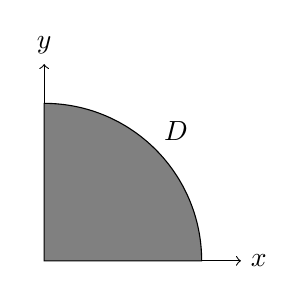
\begin{tikzpicture}
      \draw [->] (0, 0) -- (2.5, 0) node [right] {$x$};
      \draw [->] (0, 0) -- (0, 2.5) node [above] {$y$};
      \draw [fill=gray] (0, 0) -- (2, 0) arc (0:90:2) -- cycle;
      \node at (1.4, 1.4) [anchor=south west] {$D$};
    \end{tikzpicture}
  \end{center}
  Let the function to be integrated be $f = \exp(-(x^2 + y^2)/2) = \exp(-\rho^2/2)$. Then
  \begin{align*}
    \int f\;\d A &= \int f\rho\;\d\rho\;\d\varphi\\
    &=\int_{\rho=0}^R\left(\int_{\varphi=0}^{\pi/2}e^{-\rho^2/2}\rho \;\d \varphi\right)\d \rho\\
    \intertext{Note that in polar coordinates, we are integrating over a rectangle and the function is separable. So this is equal to}
    &= \left[-e^{-\rho^2/2}\right]^R_0\left[\varphi\right]_0^{\pi/2}\\
    &= \frac{\pi}{2}\left( 1 - e^{-R^2/2}\right).\tag{$*$}
  \end{align*}
  Note that the integral exists as $R\to \infty$.

  Now we take the case of $x, y\to \infty$ and consider the original integral.
  \begin{align*}
    \int _D f\;\d A &= \int_{x = 0}^{\infty} \int_{y=0}^\infty e^{-(x^2 + y^2)/2}\;\d x\;\d y\\
    &= \left(\int_0^\infty e^{-x^2/2}\;\d x\right)\left(\int_0^\infty e^{-y^2/2}\;\d y\right)\\
    &= \frac{\pi}{2}
  \end{align*}
  where the last line is from (*). So each of the two integrals must be $\sqrt{\pi/2}$, i.e.
  \[
    \int_0^\infty e^{-x^2/2}\;\d x = \sqrt{\frac{\pi}{2}}.
  \]

\end{eg}
\subsection{Generalization to \tph{$\R^3$}{R3}{&\#x211D;<sup>3</sup>}}
The definition of the area integral extends naturally to three dimensions.

\begin{defi}[Volume integral]
  Let $V \subseteq \R^3$ be a bounded region and let $f: V \to \R$ be a function. We partition $V$ into $N$ disjoint subsets (e.g., cuboids) labelled by $I$, each with volume $\delta V_I$ and contained within a sphere of diameter $\ell$. The \emph{volume integral} (or \emph{triple integral}) of $f$ over $V$ is
  \[
    \int_V f(\mathbf{r}) \, \d V = \lim_{\ell \to 0} \sum_{I} f(\mathbf{r}_I^*) \, \delta V_I,
  \]
  where $\mathbf{r}_I^*$ is a point chosen within each subset and the limit is taken as $\ell \to 0$, $N \to \infty$, with the union of subsets approaching $V$.
\end{defi}

To evaluate the integral, we use iterated integration. Taking $\delta V_I = \delta x \, \delta y \, \delta z$ and integrating successively, we obtain
\[
  \int_V f(\mathbf{r}) \, \d V = \int_D \left( \int_{Z_{xy}} f(x, y, z) \, \d z \right) \d x \, \d y,
\]
where $Z_{xy}$ denotes the range of $z$-values for each $(x, y)$ in the projection $D$ of $V$ onto the $(x, y)$-plane.

Alternatively, we may integrate over a cross-sectional area first:
\[
  \int_V f(\mathbf{r}) \, \d V = \int_Z \left( \int_{D_z} f(x, y, z) \, \d x \, \d y \right) \d z,
\]
where $D_z$ is the cross-section of $V$ at height $z$.

\begin{rmk}[Physical interpretation]
  If $f = 1$, the volume integral gives the volume of $V$. More generally, if $\rho(\mathbf{r})$ represents a density (e.g., mass density, charge density, or probability density), then $\int_V \rho(\mathbf{r}) \, \d V$ gives the total quantity contained in $V$.
\end{rmk}

\begin{defi}[Volume element]
  The \emph{volume element} is $\d V$.
\end{defi}

\begin{prop}[Cartesian volume element]
  $\d V = \d x\; \d y\; \d z$.
\end{prop}

As in two dimensions, a change of variables transforms the volume element by the absolute value of the Jacobian.

\begin{thm}[Change of variables for volume integrals]
  Let $(x, y, z) = \Phi(u, v, w)$ be a smooth, invertible transformation mapping a region $V'$ in $(u, v, w)$-space to a region $V$ in $(x, y, z)$-space. Then
  \[
    \int_V f \, \d x \, \d y \, \d z = \int_{V'} f \, |J| \, \d u \, \d v \, \d w,
  \]
  where the Jacobian is
  \[
    J = \frac{\partial(x, y, z)}{\partial(u, v, w)} =
    \begin{vmatrix}
      \dfrac{\partial x}{\partial u} & \dfrac{\partial x}{\partial v} & \dfrac{\partial x}{\partial w} \vspace{5pt}\\
      \dfrac{\partial y}{\partial u} & \dfrac{\partial y}{\partial v} & \dfrac{\partial y}{\partial w} \vspace{5pt}\\
      \dfrac{\partial z}{\partial u} & \dfrac{\partial z}{\partial v} & \dfrac{\partial z}{\partial w}
    \end{vmatrix}.
  \]
\end{thm}

\begin{prop}[Cylindrical and spherical volume elements]
  In cylindrical coordinates $(\rho, \varphi, z)$, the volume element is
  \[
    \d V = \rho \, \d\rho \, \d\varphi \, \d z.
  \]
  In spherical coordinates $(r, \theta, \varphi)$, the volume element is
  \[
    \d V = r^2 \sin\theta \, \d r \, \d\theta \, \d\varphi.
  \]
\end{prop}

\begin{proof}
  These follow from computing the Jacobians of the coordinate transformations given in Section 1.
\end{proof}

\begin{eg}[Spherical symmetry volume integral]
  Suppose $f(\mathbf{r})$ is spherically symmetric and $V$ is a sphere of radius $a$ centered on the origin. Then
  \begin{align*}
    \int_V f\;\d V &= \int_{r = 0}^a \int_{\theta = 0}^\pi \int_{\varphi = 0}^{2\pi} f(r)r^2 \sin\theta\;\d r\;\d \theta\;\d\varphi\\
    &= \int_0^a \d r\int_0^\pi \d \theta\int_0^{2\pi} \d \varphi \;r^2 f(r) \sin \theta\\
    &= \int_0^a \; r^2 f(r) \d r\Big[-\cos \theta\Big]_0^\pi \Big[\varphi\Big]_0^{2\pi}\\
    &= 4\pi\int_0^a f(r)r^2 \;\d r.
  \end{align*}
  where we separated the integral into three parts as in the area integrals.

  Note that in the second line, we rewrote the integrals to write the differentials next to the integral sign. This is simply a different notation that saves us from writing $r = 0$ etc. in the limits of the integrals.

  This is a useful general result. We understand it as the sum of spherical shells of thickness $\delta r$ and volume $4\pi r^2 \delta r$.

  If we take $f = 1$, then we have the familiar result that the volume of a sphere is $\frac{4}{3}\pi a^3$.
\end{eg}

\begin{eg}[Sphere with cylinder removed]
  Consider a volume within a sphere of radius $a$ with a cylinder of radius $b$ ($b < a$) removed. The region is defined as
  \begin{align*}
    x^2 + y^2 + z^2 &\leq a^2\\
    x^2 + y^2 &\geq b^2.
  \end{align*}
  \begin{center}
    \begin{tikzpicture}
      \begin{scope}
        \clip (-.99, 2) rectangle (-3, -2.1) (.99, 2) rectangle (3, -2.1);
        \draw circle [radius=2];
      \end{scope}
      \draw (0, 1.72) circle [x radius=1, y radius = 0.15];
      \draw [dash pattern= on 4pt off 4pt] (1, -1.72) arc (0: 180:1 and 0.15);
      \draw (-1, -1.72) arc (180: 360:1 and 0.15);
      \draw [dash pattern= on 4pt off 4pt] (1, 1.72) -- (1, -1.72);
      \draw [dash pattern= on 4pt off 4pt] (-1, 1.72) -- (-1, -1.72);
      \draw [dash pattern= on 2pt off 2pt] (0, 0) -- (1, 1.72) node [pos = 0.5, anchor = north west] {$a$};
      \draw [dash pattern= on 2pt off 2pt] (0, 0) -- (-1, 0) node [pos = 0.5, above] {$b$};
    \end{tikzpicture}
  \end{center}
  We use cylindrical coordinates. The second criteria gives
  \[
    b \leq \rho \leq a.
  \]
  For the $x^2 + y^2 + z^2 \leq a^2$ criterion, we have
  \[
    -\sqrt{a^2 - \rho^2} \leq z \leq \sqrt{a^2 - \rho^2}.
  \]
  So the volume is
  \begin{align*}
    \int_V \;\d V &= \int_b^a\d \rho\int_0^{2\pi}\d \varphi \int_{-\sqrt{a^2 - \rho^2}}^{\sqrt{a^2 - \rho^2}}\d z\; \rho\\
    &= 2\pi\int_b^a 2\rho\sqrt{a^2 - \rho^2}\;\d \rho\\
    &= 2\pi \left[-\frac{2}{3}(a^2 - \rho^2)^{3/2}\right]^a_b\\
    &= \frac{4}{3}\pi (a^2 - b^2)^{3/2}.
  \end{align*}
\end{eg}
\begin{eg}[Hemisphere total charge]
  Suppose the density of electric charge is $\rho(\mathbf{r}) = \rho_0 \frac{z}{a}$ in a hemisphere $H$ of radius $a$, with $z \geq 0$. What is the total charge of $H$?

  We use spherical polars. So
  \[
    r \leq a,\quad 0 \leq \varphi \leq 2\pi,\quad 0 \leq \theta \leq \frac{\pi}{2}.
  \]
  We have
  \[
    \rho(\mathbf{r}) = \frac{\rho_0}{a}r\cos \theta.
  \]
  The total charge $Q$ in $H$ is
  \begin{align*}
    \int_H \rho \;\d V &= \int_0^a\d r\int_0^{\pi/2}\d \theta\int_0^{2\pi}\d\varphi\; \frac{\rho_0}{a}r\cos\theta r^2\sin\theta\\
    &= \frac{\rho_0}{a}\int_0^a r^3 \;\d r \int_0^{\pi/2}\sin\theta \cos\theta\;\d \theta \int_0^{2\pi}\;\d \varphi\\
    &= \frac{\rho_0}{a}\left[\frac{r^4}{4}\right]^a_0\left[\frac{1}{2}\sin^2\theta\right]^{\pi/2}_0 [\varphi]^{2\pi}_0\\
    &= \frac{\rho_0 \pi a^3}{4}.
  \end{align*}
\end{eg}
\subsection{Further generalizations}
\subsubsection*{Integration in \tph{$\R^n$}{Rn}{&\#x2121D;<sup>n</sup>}}
The definitions and results above extend naturally to $n$ dimensions. For a region $D \subseteq \R^n$ and a function $f: D \to \R$, the $n$-dimensional integral is
\[
  \int_D f(x_1, \ldots, x_n) \, \d x_1 \cdots \d x_n.
\]

\begin{thm}[Change of variables in $\R^n$]
  Let $\mathbf{x} = \Phi(\mathbf{u})$ be a smooth, invertible transformation from $D' \subseteq \R^n$ to $D \subseteq \R^n$. Then
  \[
    \int_D f(x_1, \ldots, x_n) \, \d x_1 \cdots \d x_n = \int_{D'} f(x_1(\mathbf{u}), \ldots, x_n(\mathbf{u})) \, |J| \, \d u_1 \cdots \d u_n,
  \]
  where $J = \det\left( \frac{\partial x_i}{\partial u_j} \right)$ is the Jacobian of the transformation.
\end{thm}

\subsubsection*{Change of variables for \texorpdfstring{$n = 1$}{n = 1}}
In single-variable calculus, the change of variables formula takes a slightly different form due to the convention for definite integrals. For a transformation $x = x(u)$ mapping an interval to an interval, we have
\[
  \int_a^b f(x) \, \d x = \int_\alpha^\beta f(x(u)) \frac{\d x}{\d u} \, \d u,
\]
where $x(\alpha) = a$ and $x(\beta) = b$. Unlike in higher dimensions, we do not take the absolute value of the Jacobian; instead, the sign of $\frac{\d x}{\d u}$ accounts for the orientation of the integral.

\begin{rmk}
  If we wish to write the integral with the limits in standard order (smaller limit below), we can use
  \[
    \int_D f(x) \, \d x = \int_{D'} f(x(u)) \left| \frac{\d x}{\d u} \right| \d u,
  \]
  where the absolute value compensates for a possible reversal of orientation. This form is consistent with the higher-dimensional formula but is not the standard convention in single-variable calculus.
\end{rmk}

\subsubsection*{Vector-valued integrals}
The integral of a vector-valued function $\mathbf{F}: V \to \R^n$ over a region $V$ is defined componentwise.

\begin{defi}[Vector-valued integral]
  Let $\mathbf{F}(\mathbf{r}) = F_i(\mathbf{r}) \mathbf{e}_i$ be a vector field. The integral of $\mathbf{F}$ over a region $V$ is
  \[
    \int_V \mathbf{F}(\mathbf{r}) \, \d V = \left( \int_V F_i(\mathbf{r}) \, \d V \right) \mathbf{e}_i.
  \]
\end{defi}

\begin{eg}[Center of mass]
  For a body occupying a region $V$ with mass density $\rho(\mathbf{r})$, the total mass is
  \[
    M = \int_V \rho(\mathbf{r}) \, \d V,
  \]
  and the center of mass is
  \[
    \mathbf{R} = \frac{1}{M} \int_V \mathbf{r} \, \rho(\mathbf{r}) \, \d V.
  \]
\end{eg}
\begin{eg}[Hemisphere center of mass]
  Consider a solid hemisphere $H$ with $r \leq a$, $z \geq 0$ with uniform density $\rho$. The mass is
  \[
    M = \int_H \rho \;\d V = \frac{2}{3}\pi a^3\rho.
  \]
  Now suppose that $\mathbf{R} = (X, Y, Z)$. By symmetry, we expect $X = Y = 0$. We can find this formally by
  \begin{align*}
    X &= \frac{1}{M}\int_H x\rho \;\d V\\
    &= \frac{\rho}{M}\int_0^a \int_0^{\pi/2}\int_0^{2\pi}xr^2 \sin \theta\;\d \varphi\;\d \theta\;\d r\\
    &= \frac{\rho}{M}\int_0^{a}r^3\;\d r\times \int_0^{\pi/2}\sin^2\theta\;\d \theta\times \int_0^{2\pi}\cos\varphi\;\d \varphi\\
    &= 0
  \end{align*}
  as expected. Note that it evaluates to 0 because the integral of $\cos$ from $0$ to $2\pi$ is 0. Similarly, we obtain $Y = 0$.

  Finally, we find $Z$.
  \begin{align*}
    Z &= \frac{\rho}{M}\int_0^a r^3\;\d r \int_0^{\pi/2}\sin\theta\cos\theta\;\d \theta \int_0^{2\pi}\;\d \varphi\\
    &= \frac{\rho}{M}\left[\frac{a^4}{4}\right]\left[\frac{1}{2}\sin^2\theta\right]_0^{\pi/2}2\pi\\
    &= \frac{3a}{8}.
  \end{align*}
  So $\mathbf{R} = (0, 0, 3a/8)$.
\end{eg}

\section{Surfaces and surface integrals}
\subsection{Surfaces and Normal}
We now turn to the study of surfaces in $\R^3$. A surface can be specified implicitly by an equation of the form $f(\mathbf{r}) = c$, where $f: \R^3 \to \R$ is a smooth function and $c$ is a constant. For example, the equation $x^2 + y^2 + z^2 = 1$ defines the unit sphere.

To find the normal to such a surface, consider any curve $\mathbf{r}(u)$ lying entirely on the surface $S$. Since $f(\mathbf{r}(u)) = c$ along the curve, differentiating with respect to $u$ gives
\[
  \frac{\d}{\d u}[f(\mathbf{r}(u))] = \nabla f \cdot \frac{\d\mathbf{r}}{\d u} = 0.
\]
This shows that $\nabla f$ is perpendicular to the tangent vector $\frac{\d\mathbf{r}}{\d u}$. Since this holds for every curve on $S$, we conclude:

\begin{prop}[Gradient as surface normal]
  Let $S$ be a surface defined by $f(\mathbf{r}) = c$, where $f$ is smooth and $\nabla f \neq \mathbf{0}$ on $S$. Then $\nabla f$ is normal to $S$ at each point.
\end{prop}

\begin{eg}[Level surfaces: sphere and hyperboloid]\leavevmode
  \begin{enumerate}
    \item Take the sphere $f(\mathbf{r}) = x^2 + y^2 + z^2 = c$ for $c > 0$. Then $\nabla f = 2(x, y, z) = 2\mathbf{r}$, which is clearly normal to the sphere.
    \item Take $f(\mathbf{r}) = x^2 + y^2 - z^2 = c$, which is a hyperboloid. Then $\nabla f = 2(x, y, -z)$.

      In the special case where $c = 0$, we have a double cone, with a singular apex $\mathbf{0}$. Here $\nabla f = \mathbf{0}$, and we cannot find a meaningful direction of normal.
  \end{enumerate}
\end{eg}

\begin{defi}[Boundary of a surface]
  The \emph{boundary} of a surface $S$, denoted $\partial S$, is the curve (or union of curves) forming the edge of $S$. For example, if the upper hemisphere is defined by $x^2 + y^2 + z^2 = a^2$ with $z \geq 0$, then $\partial S$ is the circle $x^2 + y^2 = a^2$ in the plane $z = 0$.
\end{defi}

\begin{defi}[Bounded and closed surfaces]
  A surface is \emph{bounded} if it can be contained within a sphere of finite radius, and \emph{unbounded} otherwise. A bounded surface with no boundary (i.e., $\partial S = \varnothing$) is called \emph{closed}. For example, a sphere is closed, while a hemisphere is bounded but not closed.
\end{defi}
\begin{eg}[Hemisphere boundary]\leavevmode
  \begin{center}
    \begin{tikzpicture}
      \draw [draw=none, fill=gray, opacity=0.6] (-2, 0) arc (180:360:2 and 0.5) arc (0:180:2);
      \draw [mred, thick, dashed] (2, 0) arc (0:180:2 and 0.5);
      \draw [mred, thick] (-2, 0) arc (180:360:2 and 0.5);
      \draw (2, 0) arc (0:180:2);
    \end{tikzpicture}
  \end{center}
  The boundary of a hemisphere is a circle (drawn in red).
\end{eg}

\begin{defi}[Orientable surface]
  At each point of a smooth surface $S$, there are exactly two unit normal vectors, differing only in sign. A surface is \emph{orientable} if it is possible to choose a unit normal $\mathbf{n}$ at each point that varies continuously over the entire surface. Such a choice is called an \emph{orientation} of the surface.
\end{defi}

\begin{rmk}
  Most surfaces encountered in practice are orientable. For a sphere, one can choose the outward-pointing normal everywhere; for a bounded surface with boundary, one typically speaks of ``upper'' and ``lower'' or ``inward'' and ``outward'' orientations. The M\"obius strip and Klein bottle are examples of non-orientable surfaces.
\end{rmk}

\subsection{Parametrized surfaces and area}
While the implicit representation $f(\mathbf{r}) = c$ is useful for some purposes, it is often more convenient to describe a surface parametrically. A \emph{parametrization} of a surface $S$ is a smooth function $\mathbf{r}: D \to \R^3$, where $D \subseteq \R^2$ is a region in the $(u, v)$-plane, such that the image of $\mathbf{r}$ is $S$. Each point on $S$ is then labelled by coordinates $(u, v)$.

\begin{eg}[Spherical cap parametrization]
  Let $S$ be part of a sphere of radius $a$ with $0 \leq \theta \leq \alpha$.
  \begin{center}
    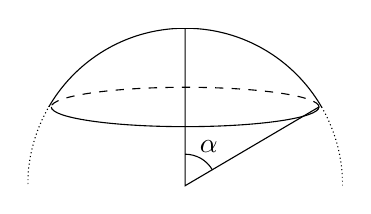
\begin{tikzpicture}
      \begin{scope}
        \clip (-2, 1) rectangle (2, 0);
        \draw [densely dotted] circle [radius=2];
      \end{scope}
      \begin{scope}
        \clip (-2, 2) rectangle (2, 1);
        \draw circle [radius=2];
      \end{scope}
      \draw [dashed] (1.7, 1) arc (0:180:1.7 and 0.25);
      \draw (-1.7, 1) arc (180:360:1.7 and 0.25);
      \draw (1.7, 1) -- (0, 0) -- (0, 2);
      \draw (0, 0.4) arc (90:30:.4);
      \node at (0.3, 0.5) {$\alpha$};
    \end{tikzpicture}
  \end{center}
  We can then label the points on the spheres by the angles $\theta, \varphi$, with
  \[
    \mathbf{r}(\theta, \varphi) = (a\cos\varphi\sin \theta, a\sin \theta\sin \varphi, a\cos \theta) = a\mathbf{e}_r.
  \]
  We restrict the values of $\theta, \varphi$ by $0 \leq \theta \leq \alpha$, $0 \leq \varphi \leq 2\pi$, so that each point is only covered once.
\end{eg}
\begin{rmk}
  A complete specification of a parametrized surface requires both the function $\mathbf{r}(u, v)$ and the domain $D \subseteq \R^2$ of allowed parameter values. The domain $D$ determines the bounds of integration when computing surface integrals.
\end{rmk}

For the parametrization to describe a genuine two-dimensional surface, we require that $\mathbf{r}$ depend non-degenerately on both parameters. The partial derivatives $\frac{\partial \mathbf{r}}{\partial u}$ and $\frac{\partial \mathbf{r}}{\partial v}$ are tangent vectors to the coordinate curves on $S$ (curves with $v$ constant and $u$ constant, respectively). For the surface to be non-degenerate, these tangent vectors must be linearly independent.

\begin{defi}[Regular parametrization]
  A parametrization $\mathbf{r}: D \to \R^3$ is called \emph{regular} if
  \[
    \frac{\partial \mathbf{r}}{\partial u} \times \frac{\partial \mathbf{r}}{\partial v} \neq \mathbf{0}
  \]
  at every point $(u, v) \in D$, i.e., the tangent vectors are never parallel. All parametrizations in this course are assumed to be regular.
\end{defi}

We now derive the formula for the area of a parametrized surface. Consider a small rectangle in the parameter domain $D$ with sides $\delta u$ and $\delta v$. Under the parametrization, this maps to a small parallelogram on $S$ with sides approximately $\frac{\partial \mathbf{r}}{\partial u} \delta u$ and $\frac{\partial \mathbf{r}}{\partial v} \delta v$. The area of this parallelogram is the magnitude of the cross product:
\[
  \delta S = \left| \frac{\partial \mathbf{r}}{\partial u} \times \frac{\partial \mathbf{r}}{\partial v} \right| \delta u \, \delta v.
\]
The cross product itself gives the \emph{vector area element}, which includes information about the orientation:
\[
  \delta \mathbf{S} = \frac{\partial \mathbf{r}}{\partial u} \times \frac{\partial \mathbf{r}}{\partial v} \, \delta u \, \delta v = \mathbf{n} \, \delta S,
\]
where $\mathbf{n}$ is the unit normal. The ordering of $u$ and $v$ determines the sign (orientation) of the normal.

Taking the limit as $\delta u, \delta v \to 0$, we obtain:
\begin{prop}[Parametrized surface area elements]
  The \emph{vector area element} is
  \[
    \d \mathbf{S} = \frac{\partial \mathbf{r}}{\partial u}\times \frac{\partial \mathbf{r}}{\partial v}\;\d u\;\d v.
  \]
  The \emph{scalar area element} is
  \[
    \d S = \left|\frac{\partial \mathbf{r}}{\partial u}\times \frac{\partial \mathbf{r}}{\partial v}\right|\;\d u\;\d v.
  \]
\end{prop}
By summing and taking limits, the area of $S$ is
\[
  \int_S \d S = \int_D \left|\frac{\partial \mathbf{r}}{\partial u}\times \frac{\partial \mathbf{r}}{\partial v}\right| \d u\;\d v.
\]
\begin{eg}[Spherical cap scalar area]
  Consider again the part of the sphere of radius $a$ with $0 \leq \theta \leq \alpha$.
  \begin{center}
    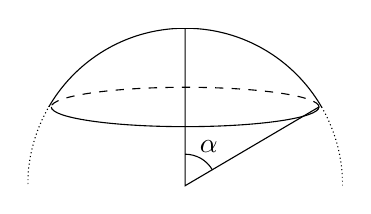
\begin{tikzpicture}
      \begin{scope}
        \clip (-2, 1) rectangle (2, 0);
        \draw [densely dotted] circle [radius=2];
      \end{scope}
      \begin{scope}
        \clip (-2, 2) rectangle (2, 1);
        \draw circle [radius=2];
      \end{scope}
      \draw [dashed] (1.7, 1) arc (0:180:1.7 and 0.25);
      \draw (-1.7, 1) arc (180:360:1.7 and 0.25);
      \draw (1.7, 1) -- (0, 0) -- (0, 2);
      \draw (0, 0.4) arc (90:30:.4);
      \node at (0.3, 0.5) {$\alpha$};
    \end{tikzpicture}
  \end{center}
  Then we have
  \[
    \mathbf{r}(\theta, \varphi) = (a\cos\varphi\sin \theta, a\sin \theta\sin \varphi, a\cos \theta) = a\mathbf{e}_r.
  \]
  So we find
  \[
    \frac{\partial \mathbf{r}}{\partial \theta} = a\mathbf{e}_\theta.
  \]
  Similarly, we have
  \[
    \frac{\partial \mathbf{r}}{\partial \varphi} = a\sin \theta \mathbf{e}_\varphi.
  \]
  Then
  \[
    \frac{\partial \mathbf{r}}{\partial \theta}\times \frac{\partial \mathbf{r}}{\partial \varphi} = a^2\sin \theta\, \mathbf{e}_r.
  \]
  So
  \[
    \d S = a^2\sin \theta\;\d \theta\;\d \varphi.
  \]
  Our bounds are $0 \leq \theta \leq \alpha$, $0 \leq \varphi \leq 2\pi$.

  Then the area is
  \[
    \int_0^{2\pi}\int_0^{\alpha} a^2\sin \theta\;\d \theta \;\d \varphi = 2\pi a^2(1 - \cos\alpha).
  \]
\end{eg}
\subsection{Surface integral of vector fields}
Having defined the area element on a surface, we now consider integrals of vector fields over surfaces. Given a surface $S$ parametrized by $\mathbf{r}(u, v)$ and a vector field $\mathbf{F}(\mathbf{r})$, we wish to measure the total ``flow'' of $\mathbf{F}$ through $S$.

A naive approach might be to integrate $|\mathbf{F}|$ over $S$, but this does not capture the physics correctly: if $\mathbf{F}$ is tangent to the surface everywhere, nothing actually passes through, yet $|\mathbf{F}|$ may be large. The correct quantity to integrate is the component of $\mathbf{F}$ normal to the surface.

\begin{defi}[Surface integral of a vector field]
  Let $S$ be an oriented surface parametrized by $\mathbf{r}: D \to \R^3$ and let $\mathbf{F}$ be a vector field. The \emph{surface integral} (or \emph{flux}) of $\mathbf{F}$ through $S$ is
  \[
    \int_S \mathbf{F} \cdot \d\mathbf{S} = \int_S \mathbf{F} \cdot \mathbf{n} \, \d S = \int_D \mathbf{F}(\mathbf{r}(u, v)) \cdot \left( \frac{\partial \mathbf{r}}{\partial u} \times \frac{\partial \mathbf{r}}{\partial v} \right) \d u \, \d v.
  \]
  This measures the net rate at which $\mathbf{F}$ crosses the surface in the direction of the chosen normal.
\end{defi}

\begin{rmk}[Parametrization independence]
  For a given orientation, the flux integral is independent of the choice of parametrization. Reversing the orientation (i.e., reversing the direction of $\mathbf{n}$) changes the sign of the integral. This is equivalent to interchanging the order of $u$ and $v$ in the parametrization.
\end{rmk}

\begin{eg}[Sphere vector area element]
  Consider a sphere of radius $a$, $\mathbf{r}(\theta, \varphi)$. Then
  \[
    \frac{\partial \mathbf{r}}{\partial \theta} = a\mathbf{e}_\theta,\quad \frac{\partial \mathbf{r}}{\partial \varphi} = a\sin \theta \mathbf{e}_\varphi.
  \]
  The vector area element is
  \[
    \d \mathbf{S} = a^2\sin \theta \mathbf{e}_r \;\d \theta\; \d\varphi,
  \]
  taking the outward normal $\mathbf{n} = \mathbf{e}_r = \mathbf{r}/a$.

  Suppose we want to calculate the fluid flux through the surface. The \emph{velocity field} $\mathbf{u}(\mathbf{r})$ of a fluid gives the motion of a small volume of fluid $\mathbf{r}$. Assume that $\mathbf{u}$ depends smoothly on $\mathbf{r}$ (and $t$). For any small area $\delta S$, on a surface $S$, the volume of fluid crossing it in time $\delta t$ is $\mathbf{u}\cdot \delta \mathbf{S}\; \delta t$.
  \begin{center}
    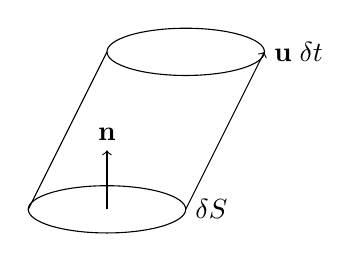
\begin{tikzpicture}
      \draw circle [x radius = 1, y radius = 0.3];
      \node at (1, 0) [right] {$\delta S$};
      \draw (1, 2) circle [x radius = 1, y radius = 0.3];
      \draw (-1, 0) -- (0, 2);
      \draw [->] (1, 0) -- (2, 2) node [right] {$\mathbf{u}\;\delta t$};
      \draw [->] (0, 0) -- (0, .75) node [above] {$\mathbf{n}$};
    \end{tikzpicture}
  \end{center}
  So the amount of flow of $\mathbf{u}$ over at time $\delta t$ through $S$ is
  \[
    \delta t\int_S \mathbf{u}\cdot \d \mathbf{S}.
  \]
  So $\int_S \mathbf{u}\cdot \d \mathbf{S}$ is the \emph{rate} of volume crossing $S$.

  For example, let $\mathbf{u} = (-x, 0, z)$ and $S$ be the section of a sphere of radius $a$ with $0 \leq \varphi \leq 2\pi$ and $0 \leq \theta \leq \alpha$. Then
  \[
    \d \mathbf{S} = a^2 \sin \theta \mathbf{n}\;\d \varphi \;\d \theta,
  \]
  with
  \[
    \mathbf{n} = \frac{\mathbf{r}}{a} = \frac{1}{a}(x, y, z).
  \]
  So
  \[
    \mathbf{n}\cdot \mathbf{u} = \frac{1}{a}(-x^2 + z^2) = a(-\sin^2\theta\cos^2\varphi + \cos^2 \theta).
  \]
  Therefore
  \begin{align*}
    \int_S \mathbf{u}\cdot \d \mathbf{S} &= \int_0^\alpha \int_0^{2\pi} a^3 \sin \theta[(\cos^2\theta - 1) \cos^2 \varphi + \cos^2 \theta]\;\d \varphi\;\d \theta\\
    &= \int_0^\alpha a^3\sin \theta[\pi(\cos^2\theta - 1) + 2\pi \cos^2\theta]\; \d \theta\\
    &=\int_0^\alpha a^3\pi(3\cos^2 \theta - 1)\sin \theta\;\d \theta\\
    &= \pi a^3[\cos\theta - \cos^3 \theta]_0^\alpha\\
    &= \pi a^3 \cos \alpha\sin^2 \alpha.
  \end{align*}
\end{eg}

We now verify that the area element is independent of the choice of parametrization. Let $\mathbf{r}(u, v)$ and $\mathbf{r}(\tilde{u}, \tilde{v})$ be two regular parametrizations for the same surface. By the chain rule,
\begin{align*}
  \frac{\partial \mathbf{r}}{\partial u} &= \frac{\partial \mathbf{r}}{\partial \tilde{u}}\frac{\partial\tilde{u}}{\partial u} + \frac{\partial \mathbf{r}}{\partial \tilde{v}}\frac{\partial\tilde{v}}{\partial u},\\
  \frac{\partial \mathbf{r}}{\partial v} &= \frac{\partial \mathbf{r}}{\partial \tilde{u}}\frac{\partial\tilde{u}}{\partial v} + \frac{\partial \mathbf{r}}{\partial \tilde{v}}\frac{\partial\tilde{v}}{\partial v}.
\end{align*}
Taking the cross product yields
\[
  \frac{\partial \mathbf{r}}{\partial u}\times\frac{\partial\mathbf{r}}{\partial v} = \frac{\partial (\tilde{u}, \tilde{v})}{\partial (u, v)} \frac{\partial \mathbf{r}}{\partial \tilde {u}}\times\frac{\partial\mathbf{r}}{\partial \tilde{v}},
\]
where $\frac{\partial (\tilde{u}, \tilde{v})}{\partial(u, v)}$ is the Jacobian of the coordinate transformation. Since the area elements in parameter space are related by
\[
  \d \tilde{u}\;\d \tilde{v} = \frac{\partial (\tilde{u}, \tilde{v})}{\partial (u, v)}\;\d u\;\d v,
\]
we obtain the following result.

\begin{prop}[Parametrization independence of area elements]
  The scalar area element is independent of the choice of parametrization:
  \[
    \d S = \left|\frac{\partial \mathbf{r}}{\partial u}\times\frac{\partial\mathbf{r}}{\partial v}\right|\;\d u\;\d v = \left|\frac{\partial \mathbf{r}}{\partial \tilde {u}}\times\frac{\partial\mathbf{r}}{\partial \tilde{v}}\right| \;\d \tilde{u}\;\d \tilde{v}.
  \]
  The vector area element
  \[
    \d \mathbf{S} = \frac{\partial \mathbf{r}}{\partial u}\times\frac{\partial\mathbf{r}}{\partial v}\;\d u\;\d v = \frac{\partial \mathbf{r}}{\partial \tilde {u}}\times\frac{\partial\mathbf{r}}{\partial \tilde{v}} \;\d \tilde{u}\;\d \tilde{v}
  \]
  is independent of parametrization provided $(u, v)$ and $(\tilde{u}, \tilde{v})$ induce the same orientation on the surface.
\end{prop}
\subsection{Change of variables in \tph{$\R^2$ and $\R^3$}{R2 and R3}{&\#x211D;<sup>2</sup> and &\#x211D;<sup>2</sup>} revisited}
The change of variables formula for integrals can be derived using the geometric ideas developed above. We present an alternative derivation that unifies the two- and three-dimensional cases.

\subsubsection*{Change of variable formula in \tph{$\R^2$}{R2}{&\#x211D;<sup>2</sup>}}
The two-dimensional change of variables formula can be derived from the surface area formula by embedding $\R^2$ in $\R^3$.

Consider a region $S \subset \R^2$ with a parametrization $(x(u, v), y(u, v))$ for $(u, v) \in D$. We embed this in $\R^3$ by setting $\mathbf{r}(u, v) = (x(u, v), y(u, v), 0)$. Computing the cross product gives
\[
  \frac{\partial \mathbf{r}}{\partial u}\times \frac{\partial\mathbf{r}}{\partial v} = (0, 0, J),
\]
where $J = \frac{\partial(x, y)}{\partial(u, v)}$ is the Jacobian of the coordinate transformation. Thus $\left|\frac{\partial \mathbf{r}}{\partial u}\times \frac{\partial\mathbf{r}}{\partial v}\right| = |J|$, and from the surface integral formula we obtain
\[
  \int_S f(x, y)\;\d S = \int_D f(x(u, v), y(u, v)) |J|\;\d u\;\d v,
\]
which is the standard change of variables formula in $\R^2$.

\subsubsection*{Change of variable formula in \tph{$\R^3$}{R3}{&\#x211D;<sup>3</sup>}}
For a volume integral in $\R^3$, we proceed similarly using the scalar triple product. Let $V$ be a region parametrized by $\mathbf{r}(u, v, w)$ for $(u, v, w) \in D$. A small displacement in parameter space gives
\[
  \delta \mathbf{r} = \frac{\partial \mathbf{r}}{\partial u}\delta u + \frac{\partial \mathbf{r}}{\partial v}\delta v + \frac{\partial \mathbf{r}}{\partial w}\delta w + o(\delta u, \delta v, \delta w).
\]
A small cuboid with sides $\delta u$, $\delta v$, $\delta w$ in parameter space maps to a parallelepiped with edges $\frac{\partial \mathbf{r}}{\partial u}\delta u$, $\frac{\partial \mathbf{r}}{\partial v}\delta v$, and $\frac{\partial \mathbf{r}}{\partial w}\delta w$. The volume of this parallelepiped is the absolute value of the scalar triple product:
\[
  \delta V = \left|\frac{\partial \mathbf{r}}{\partial u}\cdot \left( \frac{\partial \mathbf{r}}{\partial v} \times \frac{\partial \mathbf{r}}{\partial w}\right)\right| \delta u\; \delta v\;\delta w = |J|\;\delta u\; \delta v\;\delta w,
\]
where $J = \frac{\partial(x, y, z)}{\partial(u, v, w)}$ is the Jacobian. Taking the limit yields $\d V = |J|\; \d u\; \d v\; \d w$.

\section{Geometry of curves and surfaces}
We now study the intrinsic geometry of curves and surfaces, characterizing how they bend and twist in space.

\subsection{Curvature of curves}
Let $\mathbf{r}(s)$ be a curve parametrized by arclength $s$. The unit tangent vector is $\mathbf{t}(s) = \frac{\d \mathbf{r}}{\d s}$. Since $\mathbf{t}\cdot \mathbf{t} = 1$, differentiating with respect to $s$ gives $\mathbf{t}\cdot \mathbf{t}' = 0$. Thus $\mathbf{t}'$ is perpendicular to $\mathbf{t}$, i.e., $\mathbf{t}'$ is normal to the curve whenever $\mathbf{t}' \neq \mathbf{0}$.

\begin{defi}[Principal normal and curvature]
  Write $\mathbf{t}' = \kappa \mathbf{n}$, where $\mathbf{n}$ is a unit vector and $\kappa > 0$. Then $\mathbf{n}(s)$ is called the \emph{principal normal} and $\kappa(s)$ is called the \emph{curvature}.
\end{defi}

\begin{rmk}
  The curvature $\kappa$ is defined with respect to the arclength parametrization. If the curve is given in another parametrization, one must either reparametrize by arclength or use the chain rule to express derivatives with respect to $s$.
\end{rmk}

To understand the geometric meaning of curvature, we expand the curve in a Taylor series about a point. Taking $s = 0$ at the point of interest, we have
\[
  \mathbf{r}(s) = \mathbf{r}(0) + s\mathbf{r}'(0) + \frac{1}{2}s^2 \mathbf{r}''(0) + O(s^3).
\]
Since $\mathbf{r}' = \mathbf{t}$ and $\mathbf{r}'' = \mathbf{t}' = \kappa \mathbf{n}$, this becomes
\[
  \mathbf{r}(s) = \mathbf{r}(0) + s\mathbf{t}(0) + \frac{1}{2}\kappa(0) s^2 \mathbf{n}(0) + O(s^3).
\]
This expansion shows that the curve deviates from a straight line (the tangent) quadratically in $s$, with the coefficient $\kappa$ controlling the rate of deviation in the direction $\mathbf{n}$.

To interpret $\kappa$ geometrically, we compare the curve to a circle. Intuitively, a more ``curved'' curve should be approximated by a circle of smaller radius. Consider a circle of radius $a$ passing through $\mathbf{r}(0)$, lying in the plane spanned by $\mathbf{t}$ and $\mathbf{n}$:
\begin{center}
  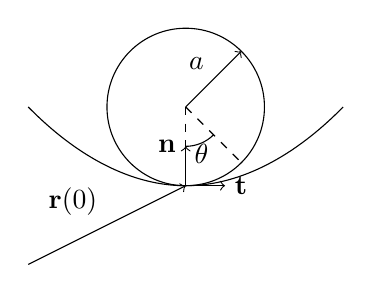
\begin{tikzpicture}
    \draw circle [radius = 1];
    \draw [->] (0, 0) -- (0.707, 0.707) node [anchor = south east, pos = 0.5] {$a$};
    \draw [->] (-2, -2) -- (0, -1) node [anchor = south east, pos = 0.5] {$\mathbf{r}(0)$};
    \draw [->] (0, -1) -- (0.5, -1) node [right] {$\mathbf{t}$};
    \draw [->] (0, -1) -- (0, -0.5) node [left] {$\mathbf{n}$};
    \draw [dashed] (0, 0) -- (0, -1);
    \draw [dashed] (0, 0) -- (0.707, -0.707);
    \draw (0, -0.5) arc (270:315:0.5);
    \node at (0.2, -0.6) {$\theta$};
    \draw (-2, 0) parabola bend (0, -1) (2, 0);
  \end{tikzpicture}
\end{center}
The parametric equation for this circle is
\[
  \mathbf{r} = \mathbf{r}(0) + a(1 - \cos \theta) \mathbf{n} + a\sin \theta \mathbf{t}.
\]
Expanding in powers of $\theta$ gives
\[
  \mathbf{r} = \mathbf{r}(0) + a\theta \mathbf{t} + \frac{1}{2}a\theta^2 \mathbf{n} + O(\theta^3).
\]
Since the arclength along the circle is $s = a\theta$, we can write $\theta = s/a$, yielding
\[
  \mathbf{r} = \mathbf{r}(0) + s\mathbf{t} + \frac{1}{2a}s^2\mathbf{n} + O(s^3).
\]
Comparing with the Taylor expansion of the curve, we see that the curve and circle agree to second order when $\kappa = 1/a$.

\begin{defi}[Osculating circle and radius of curvature]
  The \emph{osculating circle} at a point on a curve is the circle that best approximates the curve at that point (agreeing to second order in arclength). The \emph{radius of curvature} is the radius of the osculating circle, given by $1/\kappa$.
\end{defi}

\begin{prop}[Curvature and radius of curvature]
  The curvature $\kappa$ at a point on a curve equals the reciprocal of the radius of the osculating circle at that point: $\kappa = 1/a$.
\end{prop}
\subsection{The Frenet--Serret frame}
In three dimensions, the vectors $\mathbf{t}(s)$ and $\mathbf{n}(s)$ can be completed to an orthonormal basis by adding a third vector.

\begin{defi}[Binormal]
  The \emph{binormal} of a curve is the unit vector $\mathbf{b} = \mathbf{t}\times \mathbf{n}$.
\end{defi}

The ordered triple $(\mathbf{t}, \mathbf{n}, \mathbf{b})$ forms a right-handed orthonormal basis at each point of the curve, called the \emph{Frenet--Serret frame}. This frame moves along the curve with the parameter $s$.

Just as curvature measures how $\mathbf{t}$ changes along the curve, we can measure how $\mathbf{b}$ changes.

\begin{defi}[Torsion]
  The \emph{torsion} $\tau(s)$ is defined by $\mathbf{b}' = -\tau \mathbf{n}$.
\end{defi}

\begin{rmk}
  The definition is consistent because $\mathbf{b}'$ must be parallel to $\mathbf{n}$. To see this, note that $\mathbf{b}' = \mathbf{t}'\times \mathbf{n} + \mathbf{t}\times \mathbf{n}' = \mathbf{t}\times \mathbf{n}'$ (since $\mathbf{t}' = \kappa\mathbf{n}$ is parallel to $\mathbf{n}$), so $\mathbf{b}'$ is perpendicular to $\mathbf{t}$. Also, $\mathbf{b} \cdot \mathbf{b} = 1$ implies $\mathbf{b}\cdot \mathbf{b}' = 0$, so $\mathbf{b}'$ is perpendicular to $\mathbf{b}$. Thus $\mathbf{b}'$ must be parallel to $\mathbf{n}$.
\end{rmk}

The geometry of a space curve is completely determined by how the Frenet--Serret frame $(\mathbf{t}, \mathbf{n}, \mathbf{b})$ evolves along the curve. This evolution is encoded in two scalar functions of arclength: the curvature $\kappa(s)$, which measures how the curve bends in the osculating plane, and the torsion $\tau(s)$, which measures how the curve twists out of that plane.

\subsection{Curvature of surfaces*}
The geometry of surfaces can be studied through curves that lie on them. At a point $P$ on a surface $S$ with unit normal $\mathbf{n}$, consider any plane containing $\mathbf{n}$. This plane intersects $S$ in a curve passing through $P$, and this curve has some curvature $\kappa$ at $P$. Different choices of plane yield curves with different curvatures.

\begin{defi}[Principal curvatures]
  The \emph{principal curvatures} of a surface $S$ at a point $P$ are the minimum and maximum curvatures among all curves obtained by intersecting $S$ with planes containing the normal at $P$. These are denoted $\kappa_{\min}$ and $\kappa_{\max}$.
\end{defi}

\begin{defi}[Gaussian curvature]
  The \emph{Gaussian curvature} of a surface at a point $P$ is the product of the principal curvatures:
  \[
    K = \kappa_{\min}\kappa_{\max}.
  \]
\end{defi}

The following remarkable theorem, due to Gauss, reveals that Gaussian curvature has a special property.

\begin{thm}[Theorema Egregium]
  The Gaussian curvature $K$ is \emph{intrinsic} to the surface $S$: it can be expressed entirely in terms of lengths and angles measured on the surface itself, without reference to the ambient space in which $S$ is embedded.
\end{thm}

\begin{rmk}
  This theorem is the foundation of \emph{intrinsic geometry}. It implies that inhabitants of a surface can determine its Gaussian curvature purely through measurements made within the surface, without knowing how (or whether) the surface is embedded in a higher-dimensional space.
\end{rmk}

The Gaussian curvature controls deviations from Euclidean geometry on the surface. A fundamental example is the angle sum of a triangle.

\begin{defi}[Geodesic]
  A \emph{geodesic} on a surface is a curve of shortest length between two points on the surface.
\end{defi}

Consider a geodesic triangle $D$ on a surface $S$, formed by three geodesics. Let $\theta_1, \theta_2, \theta_3$ be the interior angles of the triangle, measured using scalar products of tangent vectors.

\begin{thm}[Gauss--Bonnet theorem]
  For a geodesic triangle $D$ on a surface with Gaussian curvature $K$,
  \[
    \theta_1 + \theta_2 + \theta_3 = \pi + \int_D K\; \d A.
  \]
\end{thm}

\begin{rmk}
  In Euclidean geometry ($K = 0$), the angles of a triangle sum to $\pi$. On a sphere ($K > 0$), the sum exceeds $\pi$; on a saddle surface ($K < 0$), the sum is less than $\pi$.
\end{rmk}

\section{Div, Grad, Curl and \tph{$\nabla$}{del}{&nabla;}}
\subsection{The nabla operator}
In Cartesian coordinates with orthonormal basis $\{\mathbf{e}_1, \mathbf{e}_2, \mathbf{e}_3\}$, we define the \emph{nabla} (or \emph{del}) operator as the formal vector
\[
  \nabla = \mathbf{e}_i \frac{\partial}{\partial x_i} = \left(\frac{\partial}{\partial x}, \frac{\partial }{\partial y}, \frac{\partial}{\partial z}\right).
\]
We assume the basis is right-handed, i.e., $\mathbf{e}_i\times \mathbf{e}_j = \varepsilon_{ijk} \mathbf{e}_k$.

The gradient of a scalar field $f$ is then $\nabla f$, with components $(\nabla f)_i = \frac{\partial f}{\partial x_i}$. We can also apply $\nabla$ to a vector field $\mathbf{F}(\mathbf{r}) = F_i(\mathbf{r})\mathbf{e}_i$ using the scalar or vector product, giving rise to the divergence and curl.

\begin{defi}[Divergence]
  The \emph{divergence} or \emph{div} of $\mathbf{F}$ is
  \[
    \nabla\cdot \mathbf{F} = \frac{\partial F_i}{\partial x_i} = \frac{\partial F_1}{\partial x_1} + \frac{\partial F_2}{\partial x_2} + \frac{\partial F_3}{\partial x_3}.
  \]
\end{defi}

\begin{defi}[Curl]
  The \emph{curl} of $\mathbf{F}$ is
  \[
    \nabla\times \mathbf{F} = \varepsilon_{ijk}\frac{\partial F_k}{\partial x_j}\mathbf{e}_i = \begin{vmatrix}
      \mathbf{e}_1 & \mathbf{e}_2 & \mathbf{e}_3\\
      \frac{\partial}{\partial x} & \frac{\partial}{\partial y} & \frac{\partial}{\partial z}\\
      F_x & F_y & F_z
    \end{vmatrix}
  \]
\end{defi}

\begin{eg}[Divergence and curl computation]
  Let $\mathbf{F} = (xe^z, y^2\sin x, xyz)$. Then
  \[
    \nabla \cdot \mathbf{F} = \frac{\partial }{\partial x}xe^z + \frac{\partial}{\partial y}y^2 \sin x + \frac{\partial}{\partial z}xyz = e^z + 2y\sin x + xy.
  \]
  and
  \begin{align*}
    \nabla \times F &= \hat{\mathbf{i}} \left[\frac{\partial}{\partial y}(xyz) - \frac{\partial}{\partial z}(y^2\sin x)\right]\\
    &+ \hat{\mathbf{j}} \left[\frac{\partial}{\partial z}(xe^z) - \frac{\partial}{\partial x}(xyz)\right]\\
    &+ \hat{\mathbf{k}}\left[\frac{\partial}{\partial x}(y^2\sin x) - \frac{\partial}{\partial y} (xe^z)\right]\\
    &= (xz, xe^z - yz, y^2\cos x).
  \end{align*}
\end{eg}
\begin{rmk}[Operator ordering]
  Since $\nabla$ is an operator, ordering matters. For example,
  \[
    \mathbf{F}\cdot \nabla = F_i\frac{\partial }{\partial x_i}
  \]
  is a scalar differential operator, while
  \[
    \mathbf{F}\times \nabla = \mathbf{e}_k\varepsilon_{ijk}F_i\frac{\partial}{\partial x_j}
  \]
  is a vector differential operator. These are distinct from $\nabla \cdot \mathbf{F}$ and $\nabla \times \mathbf{F}$.
\end{rmk}

\begin{prop}[Linearity of differential operators]
  Let $f, g$ be scalar fields, $\mathbf{F}, \mathbf{G}$ be vector fields, and $\lambda, \mu$ be constants. Then
  \begin{align*}
    \nabla(\lambda f + \mu g) &= \lambda\nabla f + \mu\nabla g,\\
    \nabla\cdot (\lambda \mathbf{F} + \mu \mathbf{G}) &= \lambda\nabla \cdot \mathbf{F} + \mu\nabla\cdot \mathbf{G},\\
    \nabla\times (\lambda \mathbf{F} + \mu \mathbf{G}) &= \lambda\nabla\times \mathbf{F} + \mu\nabla\times \mathbf{G}.
  \end{align*}
\end{prop}

\begin{rmk}[Dimension dependence]
  The gradient and divergence can be defined analogously in any dimension $n$, but the curl is specific to $n = 3$ because it uses the vector (cross) product.
\end{rmk}

\begin{eg}[Gradient and divergence of $r^\alpha$]
  Consider $r^\alpha$ with $r = |\mathbf{r}|$. We know that $\mathbf{r}= x_i\mathbf{e}_i$. So $r^2 = x_ix_i$. Therefore
  \[
    2r\frac{\partial r}{\partial x_j} = 2x_j,
  \]
  or
  \[
    \frac{\partial r}{\partial x_i} = \frac{x_i}{r}.
  \]
  So
  \[
    \nabla r^\alpha = \mathbf{e}_i \frac{\partial}{\partial x_i}(r^\alpha) = \mathbf{e}_i\alpha r^{\alpha - 1}\frac{\partial r}{\partial x_i} = \alpha r^{\alpha - 2}\mathbf{r}.
  \]
  Also,
  \[
    \nabla\cdot \mathbf{r} = \frac{\partial x_i}{\partial x_i} = 3.
  \]
  and
  \[
    \nabla \times \mathbf{r} = \mathbf{e}_k \varepsilon_{ijk}\frac{\partial x_j}{\partial x_i} = 0.
  \]
\end{eg}

\begin{prop}[Leibniz rules for vector operators]
  Let $f, g$ be scalar fields and $\mathbf{F}, \mathbf{G}$ be vector fields. Then
  \begin{align*}
    \nabla(fg) &= (\nabla f)g + f(\nabla g),\\
    \nabla\cdot (f\mathbf{F}) &= (\nabla f)\cdot \mathbf{F} + f(\nabla\cdot \mathbf{F}),\\
    \nabla\times (f\mathbf{F}) &= (\nabla f)\times \mathbf{F} + f(\nabla\times \mathbf{F}),\\
    \nabla(\mathbf{F}\cdot \mathbf{G}) &= \mathbf{F}\times (\nabla \times \mathbf{G}) + \mathbf{G}\times (\nabla \times \mathbf{F}) + (\mathbf{F}\cdot \nabla)\mathbf{G} + (\mathbf{G}\cdot \nabla) \mathbf{F},\\
    \nabla \times (\mathbf{F}\times \mathbf{G}) &= \mathbf{F}(\nabla\cdot \mathbf{G}) - \mathbf{G}(\nabla\cdot \mathbf{F}) + (\mathbf{G}\cdot \nabla)\mathbf{F} - (\mathbf{F}\cdot \nabla)\mathbf{G},\\
    \nabla\cdot (\mathbf{F}\times \mathbf{G}) &= (\nabla\times \mathbf{F})\cdot \mathbf{G} - \mathbf{F}\cdot (\nabla\times \mathbf{G}).
  \end{align*}
\end{prop}

\begin{proof}
  Each identity can be verified by direct computation using suffix notation and the summation convention.
\end{proof}

\begin{rmk}
  The first three identities are straightforward and worth remembering. The last three are more complex; in practice, they can be derived as needed using suffix notation.
\end{rmk}
\begin{eg}[Leibniz rules applied to $r^\alpha \mathbf{r}$]
  \begin{align*}
    \nabla\cdot (r^\alpha \mathbf{r}) &= (\nabla r^\alpha)\cdot\mathbf{r} + r^\alpha \nabla\cdot \mathbf{r}\\
    &= (\alpha r^{\alpha - 2}\mathbf{r})\cdot \mathbf{r} + r^\alpha (3)\\
    &= (\alpha + 3)r^\alpha\\
    \nabla\times (r^\alpha \mathbf{r}) &= (\nabla(r^\alpha))\times \mathbf{r} + r^\alpha(\nabla\times \mathbf{r})\\
    &= \alpha r^{\alpha - 2} \mathbf{r}\times \mathbf{r}\\
    &= \mathbf{0}
  \end{align*}
\end{eg}
\subsection{Second-order derivatives}
Two fundamental identities relate the differential operators:

\begin{prop}[Curl-grad and div-curl identities]
  For any smooth scalar field $f$ and vector field $\mathbf{F}$,
  \begin{align*}
    \nabla\times (\nabla f) &= \mathbf{0},\\
    \nabla\cdot (\nabla\times \mathbf{F}) &= 0.
  \end{align*}
\end{prop}

\begin{proof}
  Both identities follow from the symmetry of mixed partial derivatives. In suffix notation, the key observation is that
  \[
    \varepsilon_{ijk}\frac{\partial^2 f}{\partial x_i \partial x_j} = 0,
  \]
  since $\varepsilon_{ijk}$ is antisymmetric in $i, j$ while $\frac{\partial^2 f}{\partial x_i \partial x_j}$ is symmetric. For example, with $k = 3$,
  \[
    \varepsilon_{ij3}\frac{\partial^2 f}{\partial x_i \partial x_j} = \frac{\partial^2 f}{\partial x_1 \partial x_2} - \frac{\partial^2 f}{\partial x_2 \partial x_1} = 0.
  \]
\end{proof}

The converses of these identities also hold, provided the fields are defined on all of $\R^3$.

\begin{prop}[Scalar potential existence]
  If $\mathbf{F}$ is a smooth vector field defined on all of $\R^3$ with $\nabla\times \mathbf{F} = \mathbf{0}$, then there exists a scalar field $f$ such that $\mathbf{F} = \nabla f$.
\end{prop}

\begin{defi}[Conservative/irrotational field and scalar potential]
  A vector field $\mathbf{F}$ satisfying $\mathbf{F} = \nabla f$ for some scalar field $f$ is called \emph{conservative} or \emph{irrotational}. The function $f$ is called the \emph{scalar potential} of $\mathbf{F}$.
\end{defi}

\begin{prop}[Vector potential existence]
  If $\mathbf{H}$ is a smooth vector field defined on all of $\R^3$ with $\nabla\cdot \mathbf{H} = 0$, then there exists a vector field $\mathbf{A}$ such that $\mathbf{H} = \nabla \times \mathbf{A}$.
\end{prop}

\begin{defi}[Solenoidal field and vector potential]
  A vector field $\mathbf{H}$ satisfying $\mathbf{H} = \nabla \times \mathbf{A}$ for some vector field $\mathbf{A}$ is called \emph{solenoidal}. The field $\mathbf{A}$ is called the \emph{vector potential} of $\mathbf{H}$.
\end{defi}

\begin{rmk}
  The existence of scalar and vector potentials requires that the field be defined on all of $\R^3$ (or more generally, on a simply connected domain). For fields defined on domains with ``holes,'' the converse statements may fail.
\end{rmk}

\begin{defi}[Laplacian operator]
  The \emph{Laplacian operator} is defined by
  \[
    \nabla^2 = \nabla\cdot \nabla = \frac{\partial^2}{\partial x_i \partial x_i} = \left(\frac{\partial^2}{\partial x_1^2} + \frac{\partial^2}{\partial x_2^2} + \frac{\partial^2}{\partial x_3^2}\right).
  \]
  This operation is defined on both scalar and vector fields --- on a scalar field,
  \[
    \nabla^2 f = \nabla\cdot (\nabla f),
  \]
  whereas on a vector field,
  \[
    \nabla^2 \mathbf{A} = \nabla(\nabla\cdot \mathbf{A}) - \nabla\times (\nabla\times \mathbf{A}).
  \]
\end{defi}

\section{Integral theorems}
\subsection{Statement and examples}
There are three fundamental integral theorems in vector calculus: Green's theorem, Stokes' theorem, and the divergence theorem (also known as Gauss' theorem). These are all generalizations of the fundamental theorem of calculus: each states that an $n$-dimensional integral of a derivative equals an $(n-1)$-dimensional integral of the original function over the boundary.

We first state all three theorems with examples. In the following subsection, we show that the three theorems are closely related and prove them by establishing their equivalence.

\subsubsection{Green's theorem (in the plane)}
\begin{thm}[Green's theorem]
  Let $A$ be a bounded region in the $(x, y)$ plane with boundary $C = \partial A$, a piecewise smooth, non-self-intersecting closed curve traversed anticlockwise. For smooth functions $P(x, y)$ and $Q(x, y)$,
  \[
    \int_A \left(\frac{\partial Q}{\partial x} - \frac{\partial P}{\partial y}\right)\d A = \int_C P\;\d x + Q\;\d y.
  \]
\end{thm}

\begin{eg}[Green's theorem, parabola region]
  Let $Q = xy^2$ and $P = x^2y$. If $C$ is the parabola $y^2 = 4ax$ and the line $x = a$, both with $-2a \leq y \leq 2a$, then Green's theorem says
  \[
    \int_A (y^2 - x^2)\;\d A = \int_C x^2 \;\d x + xy^2\;\d y.
  \]
  From example sheet 1, each side gives $\frac{104}{105} a^4$.
\end{eg}

\begin{eg}[Green's theorem, rectangle]
  Let $A$ be a rectangle confined by $0 \leq x \leq a$ and $0 \leq y \leq b$.
  \begin{center}
    \begin{tikzpicture}
      \draw [->] (0, 0) -- (4, 0) node [right] {$x$};
      \draw [->] (0, 0) -- (0, 3) node [above] {$y$};
      \draw [->-=0.5] (0, 0) -- (3, 0) node [below] {$a$};
      \draw [->-=0.5] (3, 0) -- (3, 2);
      \draw [->-=0.5] (3, 2) -- (0, 2) node [left] {$b$};
      \draw [->-=0.5] (0, 2) -- (0, 0);
      \node at (1.5, 1) {$A$};
    \end{tikzpicture}
  \end{center}
  Then Green's theorem follows directly from the fundamental theorem of calculus in 1D. We first consider the first term of Green's theorem:
  \begin{align*}
    \int -\frac{\partial P}{\partial y} \;\d A &= \int_0^a \int_0^b -\frac{\partial P}{\partial y}\;\d y\;\d x\\
    &= \int_0^a [-P(x, b) + P(x, 0)]\;\d x\\
    &= \int_C P\;\d x
  \end{align*}
  Note that we can convert the 1D integral in the second-to-last line to a line integral around the curve $C$, since the $P(x, 0)$ and $P(x, b)$ terms give the horizontal part of $C$, and the lack of $\d y$ term means that the integral is nil when integrating the vertical parts.

  Similarly,
  \[
    \int_A \frac{\partial Q}{\partial x}\;\d A = \int_C Q\;\d y.
  \]
  Combining them gives Green's theorem.
\end{eg}

\begin{rmk}[Regions with holes]
  Green's theorem extends to bounded regions $A$ whose boundary $\partial A$ consists of multiple disconnected components (each piecewise smooth, non-self-intersecting, and closed). The exterior boundary is traversed anticlockwise, while interior boundaries (around holes) are traversed clockwise:
  \begin{center}
    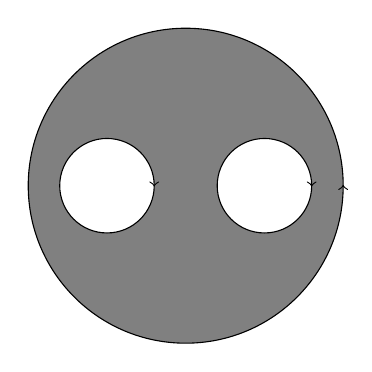
\begin{tikzpicture}
      \draw [fill = gray] circle [radius = 2];
      \draw [fill = white] (1, 0) circle [radius = 0.6];
      \draw [fill = white] (-1, 0) circle [radius = 0.6];
      \draw [->] (2, 0) -- (2, 0.01);
      \draw [->] (1.6, 0) -- (1.6, -0.01);
      \draw [->] (-0.4, 0) -- (-0.4, -0.01);
    \end{tikzpicture}
  \end{center}
  This orientation convention can be understood by imagining thin cuts connecting the boundary components, making the region simply connected, and taking the limit as the cuts shrink to zero width:
  \begin{center}
    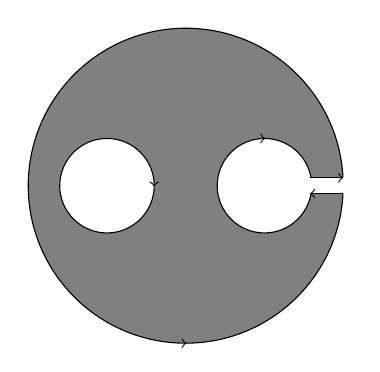
\begin{tikzpicture}
      \draw [fill = gray] circle [radius = 2];
      \draw [fill = white] (1, 0) circle [radius = 0.6];
      \draw [fill = white] (-1, 0) circle [radius = 0.6];
      \draw [->] (0, -2) -- (0.01, -2);
      \draw [->] (1, 0.6) -- (1.01, 0.6);
      \draw [->] (-0.4, 0) -- (-0.4, -0.01);
      \draw [fill = white, white] (1.5, 0.1) rectangle (2.1, -0.1);
      \draw [->] (2, -0.1) -- (1.58, -0.1);
      \draw [->] (1.58, 0.1) -- (2, 0.1);
    \end{tikzpicture}
  \end{center}
\end{rmk}

\subsubsection{Stokes' theorem}
\begin{thm}[Stokes' theorem]
  Let $S$ be a smooth, bounded, orientable surface with piecewise smooth boundary $\partial S$, and let $\mathbf{F}$ be a smooth vector field. Then
  \[
    \int_S (\nabla\times \mathbf{F})\cdot \d \mathbf{S} = \int_{\partial S} \mathbf{F}\cdot \d \mathbf{r}.
  \]
  The orientation of $\partial S$ is determined by the right-hand rule: if the thumb points in the direction of the surface normal $\mathbf{n}$, the fingers curl in the direction of traversal along $\partial S$.
\end{thm}

\begin{rmk}
  Stokes' theorem also holds when $\partial S$ consists of multiple disconnected piecewise smooth closed curves, with orientations determined as in Green's theorem.
\end{rmk}

\begin{eg}[Stokes' theorem, spherical cap]
  Let $S$ be the section of a sphere of radius $a$ with $0 \leq \theta \leq \alpha$. In spherical coordinates,
  \[
    \d \mathbf{S} = a^2 \sin \theta \mathbf{e}_r \;\d \theta\;\d \varphi.
  \]
  Let $\mathbf{F} = (0, xz, 0)$. Then $\nabla \times \mathbf{F} = (-x, 0, z)$. We have previously shown that
  \[
    \int_S \nabla\times \mathbf{F}\cdot \d \mathbf{S} = \pi a^3 \cos\alpha\sin^2 \alpha.
  \]
  Our boundary $\partial S$ is
  \[
    \mathbf{r}(\varphi) = a(\sin \alpha\cos \varphi, \sin \alpha\sin \varphi, \cos \alpha).
  \]
  The right hand side of Stokes' is
  \begin{align*}
    \int_C \mathbf{F}\cdot \d \mathbf{r} &= \int_0^{2\pi}\underbrace{a\sin \alpha\cos \varphi}_{x}\underbrace{\vphantom{\varphi}a\cos\alpha}_z \underbrace{a\sin \alpha\cos\varphi\;\d \varphi}_{\d y}\\
    &= a^3\sin^2\alpha\cos\alpha\int_0^{2\pi}\cos^2\varphi\;\d \varphi\\
    &= \pi a^3\sin^2\alpha\cos\alpha,
  \end{align*}
  which agrees with the surface integral, verifying Stokes' theorem.
\end{eg}

\subsubsection{Divergence theorem (Gauss' theorem)}
\begin{thm}[Divergence theorem]
  Let $V$ be a bounded region in $\R^3$ with piecewise smooth boundary $\partial V$, and let $\mathbf{F}$ be a smooth vector field. Then
  \[
    \int _V \nabla\cdot \mathbf{F}\;\d V = \int_{\partial V}\mathbf{F}\cdot \d \mathbf{S},
  \]
  where the surface integral is taken with respect to the outward-pointing normal.
\end{thm}

\begin{eg}[Divergence theorem, hemisphere]
  Consider a hemisphere.
  \begin{center}
    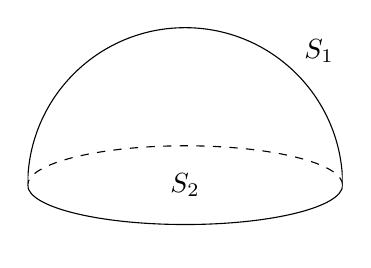
\begin{tikzpicture}
      \begin{scope}
        \clip (-2, 2) rectangle (2, 0);
        \draw circle [radius=2];
        \draw [dashed] circle [x radius = 2, y radius = 0.5];
      \end{scope}
      \begin{scope}
        \clip (-2, 0) rectangle (2, -0.7);
        \draw circle [x radius = 2, y radius = 0.5];
      \end{scope}
      \node {$S_2$};
      \node at (1.7, 1.7) {$S_1$};
    \end{tikzpicture}
  \end{center}

  $V$ is a solid hemisphere
  \[
    x^2 + y^2 + z^2 \leq a^2, \quad z \geq 0,
  \]
  and $\partial V = S_1 + S_2$, the hemisphere and the disc at the bottom.

  Take $\mathbf{F} = (0, 0, z + a)$ and $\nabla \cdot \mathbf{F} = 1$. Then
  \[
    \int_V\nabla \cdot \mathbf{F}\;\d V = \frac{2}{3}\pi a^3,
  \]
  the volume of the hemisphere.

  On $S_1$,
  \[
    \d \mathbf{S} = \mathbf{n}\;\d S = \frac{1}{a}(x, y, z)\;\d S.
  \]
  Then
  \[
    \mathbf{F}\cdot \d \mathbf{S} = \frac{1}{a}z(z + a)\;\d S = \cos \theta a(\cos \theta + 1)\underbrace{a^2\sin \theta\;\d \theta\;\d \varphi}_{\d S}.
  \]
  Then
  \begin{align*}
    \int_{S_1}\mathbf{F}\cdot \d \mathbf{S} &= a^3\int_0^{2\pi}\d \varphi \int_0^{\pi/2}\sin \theta(\cos^2\theta + \cos \theta)\;\d \theta\\
    &= 2\pi a^3 \left[\frac{-1}{3}\cos^3 \theta - \frac{1}{2}\cos^2 \theta\right]_0^{\pi/2}\\
    &= \frac{5}{3}\pi a^3.
  \end{align*}
  On $S_2$, $\d \mathbf{S} = \mathbf{n}\;\d S = -(0, 0, 1)\;\d S$. Then $\mathbf{F}\cdot \d \mathbf{S} = -a\;\d S$. So
  \[
    \int_{S_2} \mathbf{F}\cdot \d \mathbf{S} = -\pi a^3.
  \]
  So
  \[
    \int_{S_1}\mathbf{F}\cdot \d \mathbf{S} +\int_{S_2}\mathbf{F}\cdot \d \mathbf{S} = \left(\frac{5}{3} - 1\right)\pi a^3 = \frac{2}{3}\pi a^3,
  \]
  in accordance with Gauss' theorem.
\end{eg}

\subsection{Relating and proving integral theorems}
We now establish the following equivalences:
\begin{itemize}
  \item Stokes' theorem $\Leftrightarrow$ Green's theorem
  \item 2D divergence theorem $\Leftrightarrow$ Green's theorem
\end{itemize}
We then prove the 2D divergence theorem directly, which establishes all three results. The 3D divergence theorem follows by an analogous argument, though we only sketch the proof as the additional dimension makes the notation more cumbersome.

\begin{prop}[Stokes' theorem implies Green's theorem]
  Stokes' theorem $\Rightarrow$ Green's theorem.
\end{prop}

\begin{proof}
  Green's theorem concerns regions in $\R^2$, while Stokes' theorem concerns surfaces in $\R^3$. We derive Green's theorem by applying Stokes' theorem to a planar surface.

  Let $A$ be a region in the $(x, y)$ plane with boundary $C = \partial A$, parametrised by arc length, $(x(s), y(s), 0)$. Then the tangent to $C$ is
  \[
    \mathbf{t} = \left(\frac{\d x}{\d s}, \frac{\d y}{\d s}, 0\right).
  \]
  Given any $P(x, y)$ and $Q(x, y)$, we can consider the vector field
  \[
    \mathbf{F} = (P, Q, 0),
  \]
  So
  \[
    \nabla \times \mathbf{F} = \left(0, 0, \frac{\partial Q}{\partial x} - \frac{\partial P}{\partial y}\right).
  \]
  The line integral in Stokes' theorem becomes
  \[
    \int_C \mathbf{F} \cdot \d \mathbf{r} = \int_C \mathbf{F}\cdot \mathbf{t}\;\d s = \int_C P\;\d x + Q\;\d y,
  \]
  and the surface integral (with $\d\mathbf{S} = \hat{\mathbf{k}}\,\d A$ for a surface in the $xy$-plane) becomes
  \[
    \int_A (\nabla\times \mathbf{F})\cdot \hat{\mathbf{k}}\;\d A = \int_A \left(\frac{\partial Q}{\partial x} - \frac{\partial P}{\partial y}\right)\d A.\qedhere
  \]
\end{proof}

\begin{prop}[Green's theorem implies Stokes' theorem]
  Green's theorem $\Rightarrow$ Stokes' theorem.
\end{prop}

\begin{proof}
  Green's theorem concerns a 2D region, while Stokes' theorem concerns a 3D surface $S$ parametrized by $\mathbf{r}(u, v)$. We apply Green's theorem in the parameter space $(u, v)$.

  Consider a parametrised surface $S = \mathbf{r}(u, v)$ corresponding to the region $A$ in the $u, v$ plane. Write the boundary as $\partial A = (u(t), v(t))$. Then $\partial S = \mathbf{r}(u(t), v(t))$.

  We want to prove
  \[
    \int_{\partial S}\mathbf{F}\cdot \d \mathbf{r} = \int_S (\nabla \times \mathbf{F})\cdot \d \mathbf{S}
  \]
  given
  \[
    \int_{\partial A} F_u\;\d u + F_v\;\d v = \int_A\left(\frac{\partial F_v}{\partial u} - \frac{\partial F_u}{\partial v}\right)\;\d A.
  \]
  Doing some pattern-matching, we want
  \[
    \mathbf{F}\cdot \d \mathbf{r} = F_u \;\d u + F_v \;\d v
  \]
  for some $F_u$ and $F_v$.

  By the chain rule, we know that
  \[
    \d \mathbf{r} = \frac{\partial \mathbf{r}}{\partial u} \d u + \frac{\partial \mathbf{r}}{\partial v}\d v.
  \]
  So we choose
  \[
    F_u = \mathbf{F}\cdot \frac{\partial \mathbf{r}}{\partial u}, \quad F_v = \mathbf{F}\cdot\frac{\partial \mathbf{r}}{\partial v}.
  \]
  This choice matches the left hand sides of the two equations.

  To match the right, recall that
  \[
    (\nabla\times \mathbf{F}) \cdot \d \mathbf{S} = (\nabla\times \mathbf{F})\cdot \left(\frac{\partial \mathbf{r}}{\partial u}\times \frac{\partial \mathbf{r}}{\partial v}\right)\;\d u\;\d v.
  \]
  For the right-hand sides to match, we need
  \[
    \frac{\partial F_v}{\partial u} - \frac{\partial F_u}{\partial v} = (\nabla\times \mathbf{F})\cdot \left(\frac{\partial \mathbf{r}}{\partial u}\times \frac{\partial \mathbf{r}}{\partial v}\right).\tag{$*$}
  \]
  We verify this using suffix notation:
  \[
    \frac{\partial F_v}{\partial u} = \frac{\partial}{\partial u}\left(\mathbf{F}\cdot \frac{\partial \mathbf{r}}{\partial v}\right) = \frac{\partial}{\partial u}\left(F_i\frac{\partial x_i}{\partial v}\right) = \left(\frac{\partial F_i}{\partial x_j}\frac{\partial x_j}{\partial u}\right)\frac{\partial x_i}{\partial v} + F_i\frac{\partial x_i}{\partial u\partial v}.
  \]
  Similarly,
  \[
    \frac{\partial F_u}{\partial v} = \frac{\partial}{\partial v}\left(\mathbf{F}\cdot \frac{\partial \mathbf{r}}{\partial u}\right) = \frac{\partial}{\partial v}\left(F_j\frac{\partial x_j}{\partial u}\right) = \left(\frac{\partial F_j}{\partial x_i}\frac{\partial x_i}{\partial v}\right)\frac{\partial x_j}{\partial u} + F_i\frac{\partial x_i}{\partial u\partial v}.
  \]
  So
  \[
    \frac{\partial F_v}{\partial u} - \frac{\partial F_u}{\partial v} = \frac{\partial x_j}{\partial u}\frac{\partial x_i}{\partial v}\left(\frac{\partial F_i}{\partial x_j} - \frac{\partial F_j}{\partial x_i}\right).
  \]
  This is the left hand side of $(*)$.

  The right hand side of $(*)$ is
  \begin{align*}
    (\nabla \times \mathbf{F})\cdot \left(\frac{\partial \mathbf{r}}{\partial u}\times \frac{\partial \mathbf{r}}{\partial v}\right) &= \varepsilon_{ijk}\frac{\partial F_j}{\partial x_i}\varepsilon_{kpq}\frac{\partial x_p}{\partial u}\frac{\partial x_q}{\partial v}\\
    &= (\delta_{ip}\delta_{jq} - \delta_{iq}\delta_{jp}) \frac{\partial F_j}{\partial x_i}\frac{\partial x_p}{\partial u}\frac{\partial x_q}{\partial v}\\
    &= \left(\frac{\partial F_j}{\partial x_i} - \frac{\partial F_i}{\partial x_j}\right)\frac{\partial x_i}{\partial u}\frac{\partial x_j}{\partial v}.
  \end{align*}
  The two expressions match, so with this choice of $F_u$ and $F_v$, Green's theorem implies Stokes' theorem.
\end{proof}

\begin{prop}[Green's theorem $\Leftrightarrow$ 2D divergence theorem]
  Green's theorem and the 2D divergence theorem are equivalent.
\end{prop}

\begin{proof}
  The 2D divergence theorem states that
  \[
    \int_A (\nabla\cdot \mathbf{G})\;\d A = \int_{\partial A} \mathbf{G}\cdot \mathbf{n}\;\d s,
  \]
  where $\mathbf{n}$ is the outward-pointing normal.

  Given functions $P$ and $Q$, set $\mathbf{G} = (Q, -P)$. Then
  \[
    \nabla\cdot \mathbf{G} = \frac{\partial Q}{\partial x} - \frac{\partial P}{\partial y}.
  \]
  Around the curve $\mathbf{r}(s) = (x(s), y(s))$, $\mathbf{t}(s) = (x'(s), y'(s))$. Then the normal, being perpendicular to $\mathbf{t}$, is $\mathbf{n}(s) = (y'(s), -x'(s))$ (check that it points outwards!). So
  \[
    \mathbf{G}\cdot \mathbf{n} = P\frac{\d x}{\d s} + Q\frac{\d y}{\d s}.
  \]
  Then we can expand out the integrals to obtain
  \[
    \int_C \mathbf{G}\cdot \mathbf{n}\;\d s = \int_C P\;\d x + Q\;\d y,
  \]
  and
  \[
    \int_A(\nabla\cdot \mathbf{G})\;\d A = \int_A\left(\frac{\partial Q}{\partial x} - \frac{\partial P}{\partial y}\right)\;\d A.
  \]
  The 2D divergence theorem asserts that the two left-hand sides are equal, while Green's theorem asserts that the two right-hand sides are equal. Thus the two theorems are equivalent.
\end{proof}

\begin{prop}[2D divergence theorem]
  Let $A$ be a bounded region in $\R^2$ with piecewise smooth boundary $C = \partial A$. For a smooth vector field $\mathbf{G}$,
  \[
    \int_A (\nabla\cdot \mathbf{G})\;\d A = \int_C \mathbf{G}\cdot \mathbf{n}\;\d s,
  \]
  where $\mathbf{n}$ is the outward-pointing unit normal.
\end{prop}

\begin{proof}
  By linearity, it suffices to prove the result for vector fields with only a vertical component; the horizontal case is analogous, and the general case follows by superposition.

  We also assume that $A$ is a simple convex region. More complicated regions can be decomposed into simple pieces, and the theorem applied to each piece.

  Suppose $\mathbf{G} = G(x, y)\hat{\mathbf{j}}$. Then
  \[
    \nabla \cdot \mathbf{G} = \frac{\partial G}{\partial y}.
  \]
  Then
  \[
    \int_A \nabla\cdot \mathbf{G}\;\d A = \int_X \left(\int_{Y_x}\frac{\partial G}{\partial y}\;\d y\right)\;\d x.
  \]
  Divide the boundary $C$ into upper and lower parts, $C_+$ and $C_-$, described by $y = y_+(x)$ and $y = y_-(x)$ respectively:
  \begin{center}
    \begin{tikzpicture}
      \draw [red] (3, 1.5) arc (0:180:1);
      \node [red, anchor = south east] at (1.2, 1.75) {$C_+$};
      \draw [blue] (1, 1.5) arc (180:360:1);
      \node [blue, anchor = north west] at (3, 1.5) {$C_-$};

      \draw (1.8, 0.52) -- (1.8, 2.48);
      \draw (2.2, 0.52) -- (2.2, 2.48);
      \draw [dashed] (1.8, 0.52) -- (1.8, 0);
      \draw [dashed] (2.2, 0.52) -- (2.2, 0);
      \node [below] at (2, 0) {$\d y$};

      \draw [dashed] (1.8, 0.52) -- (0, 0.52);
      \draw [dashed] (1.8, 2.48) -- (0, 2.48);
      \draw [->] (-0.3, 2.48) -- (-0.3, 0.52);
      \draw [->] (-0.3, 0.52) -- (-0.3, 2.48) node [pos = 0.5, fill=white] {$Y_x$};

      \draw [->] (0, 0) -- (5, 0) node [right] {$x$};
      \draw [->] (0, 0) -- (0, 3) node [above] {$y$};
    \end{tikzpicture}
  \end{center}
  We see that the boundary of $Y_x$ at any specific $x$ is given by $y_-(x)$ and $y_+(x)$. Hence by the Fundamental theorem of Calculus,
  \[
    \int_{Y_x}\frac{\partial G}{\partial y}\;\d y = \int_{y_-(x)}^{y_+(x)} \frac{\partial G}{\partial y}\;\d y = G(x, y_+(x)) - G(x, y_-(x)).
  \]
  To compute the full area integral, we want to integrate over all $x$. However, the divergence theorem talks in terms of $\d s$, not $\d x$. So we need to find some way to relate $\d s$ and $\d x$. If we move a distance $\delta s$, the change in $x$ is $\delta s\cos \theta$, where $\theta$ is the angle between the tangent and the horizontal. But $\theta$ is also the angle between the normal and the vertical. So $\cos \theta = \mathbf{n}\cdot \hat{\mathbf{j}}$. Therefore $\d x = \hat{\mathbf{j}}\cdot \mathbf{n}\;\d s$.

  In particular, $G\;\d x = G\,\hat{\mathbf{j}}\cdot \mathbf{n}\;\d s = \mathbf{G}\cdot \mathbf{n}\;\d s$, since $\mathbf{G} = G\,\hat{\mathbf{j}}$.

  However, at $C_-$, $\mathbf{n}$ points downwards, so $\mathbf{n}\cdot \hat{\mathbf{j}}$ happens to be negative. So, actually, at $C_-$, $\d x = -\mathbf{G}\cdot \mathbf{n}\;\d s$.

  Therefore, our full integral is
  \begin{align*}
    \int_A \nabla\cdot \mathbf{G}\;\d A &= \int_X \left(\int_{y_x}\frac{\partial G}{\partial y}\;\d Y\right)\;\d x\\
    &= \int_X G(x, y_+(x)) - G(x, y_{-}(x))\;\d x\\
    &= \int_{C_+}\mathbf{G}\cdot \mathbf{n}\;\d s + \int_{C_-}\mathbf{G}\cdot \mathbf{n}\;\d s\\
    &= \int_C \mathbf{G}\cdot \mathbf{n}\;\d s.\qedhere
  \end{align*}
\end{proof}

\begin{rmk}[Sketch of 3D divergence theorem proof]
  The 3D divergence theorem is proved analogously. Consider a purely vertical vector field $\mathbf{F} = F(x, y, z)\hat{\mathbf{k}}$. Then
  \[
    \int_V \nabla\cdot \mathbf{F}\;\d V = \int_D \left(\int_{Z_{xy}} \frac{\partial F}{\partial z}\;\d z\right)\d A,
  \]
  where $D$ is the projection of $V$ onto the $xy$-plane and $Z_{xy}$ is the range of $z$ values above each point $(x, y) \in D$. Splitting $S = \partial V$ into top and bottom parts $S_+$ and $S_-$ (where $\hat{\mathbf{k}}\cdot \mathbf{n} \geq 0$ and $\hat{\mathbf{k}}\cdot \mathbf{n} < 0$ respectively), parametrized by $z = z_+(x, y)$ and $z = z_-(x, y)$, the integral becomes
  \[
    \int_V \nabla\cdot \mathbf{F}\;\d V = \int_D (F(x, y, z_+) - F(x, y, z_-))\;\d A = \int_S \mathbf{F}\cdot \mathbf{n}\;\d S.
  \]
  The general case follows by decomposing $\mathbf{F}$ into components along each coordinate axis.
\end{rmk}
\section{Some applications of integral theorems}
\subsection{Integral expressions for div and curl}
The integral theorems provide coordinate-free definitions of divergence and curl that clarify their geometric meaning.

Applying the divergence theorem to a small volume $V$ containing a point $\mathbf{r}_0$,
\[
  \int_{\partial V}\mathbf{F}\cdot \d \mathbf{S} = \int_V\nabla\cdot \mathbf{F}\;\d V\approx (\nabla\cdot \mathbf{F})(\mathbf{r}_0) \vol(V).
\]
Taking the limit as $V$ shrinks to $\mathbf{r}_0$ yields:

\begin{prop}[Integral definition of divergence]
  \[
    (\nabla \cdot \mathbf{F})(\mathbf{r}_0) = \lim_{\mathrm{diam}(V) \to 0} \frac{1}{\vol(V)}\int_{\partial V}\mathbf{F}\cdot \d \mathbf{S},
  \]
  where the limit is taken over volumes $V$ containing $\mathbf{r}_0$.
\end{prop}

Similarly, applying Stokes' theorem to a small surface $A$ containing $\mathbf{r}_0$ with unit normal $\mathbf{n}$,
\[
  \int _{\partial A}\mathbf{F}\cdot \d \mathbf{r} = \int_A(\nabla\times \mathbf{F})\cdot \mathbf{n}\;\d A \approx \mathbf{n}\cdot (\nabla\times \mathbf{F})(\mathbf{r}_0) \area(A).
\]

\begin{prop}[Integral definition of curl]
  \[
    \mathbf{n}\cdot (\nabla \times \mathbf{F})(\mathbf{r}_0) = \lim_{\mathrm{diam}(A) \to 0}\frac{1}{\area(A)}\int_{\partial A}\mathbf{F}\cdot \d \mathbf{r},
  \]
  where the limit is taken over surfaces $A$ containing $\mathbf{r}_0$ with normal $\mathbf{n}$.
\end{prop}

\begin{rmk}
  These definitions are independent of the choice of coordinate system and provide the basis for physical interpretations of divergence and curl.
\end{rmk}

\begin{eg}[Fluid flow interpretation of divergence and curl]
  Let $\mathbf{u}$ be the velocity field of a fluid flow. The flux integral $\int_S \mathbf{u}\cdot \d \mathbf{S}$ gives the rate at which fluid crosses the surface $S$.

  \emph{Divergence as expansion rate:} Consider a small volume $V$ of fluid. The rate of change of its volume is
  \[
    \dot{V} = \int_{\partial V}\mathbf{u}\cdot \d \mathbf{S}.
  \]
  By the integral definition of divergence,
  \[
    \nabla\cdot \mathbf{u} = \lim_{V\to 0}\frac{\dot{V}}{V},
  \]
  which is the relative rate of volume expansion. For example, if $\mathbf{u}(\mathbf{r}) = \alpha\mathbf{r}$ (radial outflow from the origin), then $\nabla\cdot \mathbf{u} = 3\alpha$, indicating uniform expansion throughout space.

  \emph{Curl as rotation rate:} Consider a disc $A$ of radius $a$ with unit normal $\mathbf{n}$. The circulation around its boundary is
  \[
    \int_{\partial A}\mathbf{u}\cdot \d \mathbf{r} = \int_{\partial A}\mathbf{u}\cdot \mathbf{t} \;\d s = 2\pi a \times (\text{average tangential velocity}).
  \]
  Define the local angular velocity as
  \[
    \omega = \frac{1}{a} \times (\text{average of }\mathbf{u}\cdot \mathbf{t}).
  \]
  As $a \to 0$, the average tangential velocity decreases (a smooth field varies less on smaller scales), but the ratio $\omega$ approaches a finite limit. Since $\int_{\partial A} \mathbf{u}\cdot \d \mathbf{r} = 2\pi a^2 \omega$, the integral definition gives
  \[
    \mathbf{n}\cdot (\nabla \times \mathbf{u}) = \lim_{a \to 0}\frac{1}{\pi a^2}\int_{\partial A}\mathbf{u}\cdot \d \mathbf{r} = 2\omega.
  \]
  Thus the curl measures twice the local angular velocity of the fluid. For rigid body rotation with angular velocity $\boldsymbol\omega$, the velocity field is $\mathbf{u} = \boldsymbol\omega\times \mathbf{r}$, and
  \[
    \nabla\times (\boldsymbol\omega\times \mathbf{r}) = 2\boldsymbol\omega.
  \]
\end{eg}

\subsection{Conservative fields and scalar potentials}
\begin{defi}[Conservative field]
  A vector field $\mathbf{F}$ is \emph{conservative} if any of the following equivalent conditions holds:
  \begin{enumerate}
    \item $\mathbf{F} = \nabla f$ for some scalar field $f$ (called the \emph{scalar potential});
    \item $\int_C \mathbf{F}\cdot \d \mathbf{r}$ depends only on the endpoints of $C$, not on the path;
    \item $\nabla \times \mathbf{F} = \mathbf{0}$.
  \end{enumerate}
\end{defi}

We now prove these conditions are equivalent. The implications (i) $\Rightarrow$ (ii) and (i) $\Rightarrow$ (iii) were established earlier:
\[
  \text{(i) } \Rightarrow \text{ (ii):} \quad \int_C \mathbf{F}\cdot \d \mathbf{r} = f(\mathbf{b}) - f(\mathbf{a}), \qquad
  \text{(i) } \Rightarrow \text{ (iii):} \quad \nabla \times (\nabla f) = \mathbf{0}.
\]
It remains to show (iii) $\Rightarrow$ (ii) and (ii) $\Rightarrow$ (i).
\begin{prop}[Path independence, sufficient condition]
  If (iii) $\nabla\times \mathbf{F}= 0 $, then (ii) $\int_C \mathbf{F}\cdot \d \mathbf{r}$ is independent of $C$.
\end{prop}

\begin{proof}
  Given $\mathbf{F}(\mathbf{r})$ satisfying $\nabla\times \mathbf{F} = 0$, let $C$ and $\tilde C$ be any two curves from $\mathbf{a}$ to $\mathbf{b}$.
  \begin{center}
    \begin{tikzpicture}
      \node [circ] {};
      \node [left] {$\mathbf{a}$};
      \node at (2, 2) [circ] {};
      \node at (2, 2) [right] {$\mathbf{b}$};
      \node at (2, 1) {$\tilde C$};
      \draw [->-=0.6] plot [smooth, tension=1] coordinates {(0, 0) (0.8, 1.7) (2, 2)};
      \node [above] at (0.8, 1.7) {$C$};
      \draw [->-=0.6] plot [smooth, tension=1] coordinates {(0, 0) (1.2, -0.1) (2, 2)};
    \end{tikzpicture}
  \end{center}
  If $S$ is any surface with boundary $\partial S = C - \tilde C$, By Stokes' theorem,
  \[
    \int_{S}\nabla \times \mathbf{F}\cdot \d \mathbf{S} = \int_{\partial S}\mathbf{F}\cdot \d \mathbf{r} = \int_C \mathbf{F}\cdot \d \mathbf{r} - \int_{\tilde{C}}\mathbf{F}\cdot \d \mathbf{r}.
  \]
  But $\nabla\times \mathbf{F} = 0$. So
  \[
    \int_C \mathbf{F}\cdot \d \mathbf{r} - \int_{\tilde{C}} \mathbf{F}\cdot \d \mathbf{r} = 0,
  \]
  or
  \[
    \int_C \mathbf{F}\cdot \d \mathbf{r} = \int_{\tilde{C}}\mathbf{F}\cdot \d \mathbf{r}.\qedhere
  \]
\end{proof}

\begin{prop}[Path independence, necessary condition]
  If (ii) $\int_C \mathbf{F}\cdot \d \mathbf{r}$ is independent of $C$ for fixed end points and orientation, then (i) $\mathbf{F} = \nabla f$ for some scalar field $f$.
\end{prop}

\begin{proof}
  We fix $\mathbf{a}$ and define $f(\mathbf{r}) = \int_C \mathbf{F}(\mathbf{r}')\cdot\d \mathbf{r}'$ for any curve from $\mathbf{a}$ to $\mathbf{r}$. Assuming (ii), $f$ is well-defined. For small changes $\mathbf{r}$ to $\mathbf{r} + \delta \mathbf{r}$, there is a small extension of $C$ by $\delta C$. Then
  \begin{align*}
    f(\mathbf{r} + \delta \mathbf{r}) &= \int_{C + \delta C}\mathbf{F} (\mathbf{r}')\cdot \d \mathbf{r}'\\
    &= \int_C \mathbf{F}\cdot \d \mathbf{r}' + \int_{\delta C}\mathbf{F}\cdot \d \mathbf{r}'\\
    &= f(\mathbf{r}) + \mathbf{F}(\mathbf{r})\cdot \delta \mathbf{r} + o(\delta \mathbf{r}).
  \end{align*}
  So
  \[
    \delta f = f(\mathbf{r} + \delta \mathbf{r}) - f(\mathbf{r}) = \mathbf{F}(\mathbf{r})\cdot \delta \mathbf{r} + o(\delta \mathbf{r}).
  \]
  But the definition of grad is exactly
  \[
    \delta f = \nabla f\cdot \delta \mathbf{r} + o(\delta \mathbf{r}).
  \]
  So we have $\mathbf{F} = \nabla f$.
\end{proof}

\begin{rmk}[Simply connected domains]
  The above results assume $\mathbf{F}$ is defined on all of $\R^3$, but they also hold on any \emph{simply connected} domain $D$. A domain is simply connected if any closed loop can be continuously shrunk to a point, or equivalently, if any two curves with the same endpoints can be smoothly deformed into one another.

  The proof that (iii) $\Rightarrow$ (ii) requires the existence of a surface $S$ bounded by $C - \tilde{C}$. Such a surface exists precisely when $C$ and $\tilde{C}$ can be deformed into each other.

  If $D$ is not simply connected, a scalar potential $f$ may be multi-valued. However, one can often restrict to a simply connected subset $D_0 \subseteq D$ on which $f$ is single-valued.
\end{rmk}

\begin{eg}[Multi-valued potential on a non-simply-connected domain]
  Consider the vector field
  \[
    \mathbf{F} = \left(\frac{-y}{x^2 + y^2}, \frac{x}{x^2 + y^2}, 0\right),
  \]
  defined on $D = \R^3 \setminus \{z\text{-axis}\}$, which is not simply connected. One can verify that $\nabla\times \mathbf{F} = \mathbf{0}$ on $D$. Formally, $\mathbf{F} = \nabla f$ where
  \[
    f = \arctan\frac{y}{x},
  \]
  but this potential is multi-valued (the arctangent has multiple branches).

  The non-trivial topology manifests when we integrate around the unit circle $x^2 + y^2 = 1$ in the $z = 0$ plane:
  \[
    \oint_C \mathbf{F}\cdot \d\mathbf{r} = 2\pi \neq 0.
  \]
  For a truly conservative field, all closed loop integrals would vanish.

  To obtain a single-valued potential, we can restrict to the simply connected domain
  \[
    D_0 = \R^3 \setminus \{(x, y, z) : x \leq 0,\, y = 0\},
  \]
  obtained by removing a half-plane. On $D_0$, no closed curve can encircle the $z$-axis, and the potential becomes single-valued.
\end{eg}

\subsection{Conservation laws}
\begin{defi}[Continuity equation]
  Let $\rho(\mathbf{r}, t)$ be the density (amount per unit volume) of some conserved quantity, and let $\mathbf{j}(\mathbf{r}, t)$ be the corresponding flux density (flow rate per unit area). The \emph{continuity equation} (or \emph{conservation equation}) is
  \[
    \frac{\partial \rho}{\partial t} + \nabla\cdot \mathbf{j} = 0.
  \]
\end{defi}

This equation expresses \emph{local} conservation: the quantity cannot appear or disappear, but must flow continuously from place to place.

\begin{prop}[Integral form of conservation]
  Let $V$ be a fixed region with boundary $S = \partial V$, and let $Q(t) = \int_V \rho(\mathbf{r}, t)\, \d V$ be the total amount of the conserved quantity in $V$. Then
  \[
    \frac{\d Q}{\d t} = -\int_S \mathbf{j}\cdot \d \mathbf{S}.
  \]
\end{prop}

\begin{proof}
  By the continuity equation and the divergence theorem,
  \[
    \frac{\d Q}{\d t} = \int_V \frac{\partial \rho}{\partial t}\,\d V = -\int_V \nabla \cdot \mathbf{j}\,\d V = -\int_S \mathbf{j}\cdot \d \mathbf{S}.\qedhere
  \]
\end{proof}

This states that the rate of change of $Q$ in $V$ equals the net inward flux through the boundary: the quantity cannot disappear from $V$ except by flowing out through $\partial V$.

\begin{rmk}[Global conservation]
  If $\mathbf{j} \to \mathbf{0}$ sufficiently rapidly as $|\mathbf{r}| \to \infty$, then taking $V$ to be all of $\R^3$ (as a limit of large spheres) gives $\frac{\d Q_{\text{total}}}{\d t} = 0$: the total amount of the quantity in the universe is constant.
\end{rmk}
\begin{eg}[Charge conservation]
  Let $\rho(\mathbf{r}, t)$ be the electric charge density and $\mathbf{j}(\mathbf{r}, t)$ be the current density. The continuity equation
  \[
    \frac{\partial \rho}{\partial t} + \nabla\cdot \mathbf{j} = 0
  \]
  expresses conservation of electric charge: charge can only change in a region by flowing in or out as current.
\end{eg}

\begin{eg}[Mass conservation and incompressibility]
  For a fluid with mass density $\rho(\mathbf{r}, t)$ and velocity field $\mathbf{u}(\mathbf{r}, t)$, the mass flux is $\mathbf{j} = \rho \mathbf{u}$. The continuity equation becomes
  \[
    \frac{\partial \rho}{\partial t} + \nabla\cdot (\rho \mathbf{u}) = 0,
  \]
  which is the equation of mass conservation for a fluid.

  For an \emph{incompressible} fluid, the density $\rho$ is constant (independent of $\mathbf{r}$ and $t$). The continuity equation then reduces to
  \[
    \nabla\cdot \mathbf{u} = 0,
  \]
  stating that the velocity field is divergence-free.
\end{eg}

\section{Orthogonal curvilinear coordinates}
\subsection{Line, area and volume elements}
A coordinate system provides a way to specify points in space using a set of numbers. In three dimensions, we describe a coordinate system by a smooth, invertible function $\mathbf{r}(u, v, w)$ mapping coordinate values to position vectors. By the chain rule,
\[
  \d \mathbf{r} = \frac{\partial \mathbf{r}}{\partial u}\,\d u + \frac{\partial \mathbf{r}}{\partial v}\,\d v + \frac{\partial \mathbf{r}}{\partial w}\,\d w.
\]
For the coordinates to be non-degenerate, the tangent vectors $\frac{\partial \mathbf{r}}{\partial u}$, $\frac{\partial \mathbf{r}}{\partial v}$, $\frac{\partial \mathbf{r}}{\partial w}$ must be linearly independent at each point, i.e.,
\[
  \frac{\partial \mathbf{r}}{\partial u}\cdot \left(\frac{\partial \mathbf{r}}{\partial v}\times \frac{\partial \mathbf{r}}{\partial w}\right) \neq 0.
\]
These tangent vectors point along the coordinate curves (curves where two coordinates are held fixed).

\begin{defi}[Orthogonal curvilinear coordinates]
  Coordinates $(u, v, w)$ are \emph{orthogonal curvilinear coordinates} if the tangent vectors $\frac{\partial \mathbf{r}}{\partial u}$, $\frac{\partial \mathbf{r}}{\partial v}$, $\frac{\partial \mathbf{r}}{\partial w}$ are mutually orthogonal at every point.
\end{defi}

\begin{defi}[Scale factors]
  For orthogonal curvilinear coordinates, the \emph{scale factors} $h_u$, $h_v$, $h_w$ are defined by
  \[
    h_u = \left|\frac{\partial \mathbf{r}}{\partial u}\right|, \quad h_v = \left|\frac{\partial \mathbf{r}}{\partial v}\right|, \quad h_w = \left|\frac{\partial \mathbf{r}}{\partial w}\right|.
  \]
  The corresponding unit vectors are
  \[
    \mathbf{e}_u = \frac{1}{h_u}\frac{\partial \mathbf{r}}{\partial u}, \quad \mathbf{e}_v = \frac{1}{h_v}\frac{\partial \mathbf{r}}{\partial v}, \quad \mathbf{e}_w = \frac{1}{h_w}\frac{\partial \mathbf{r}}{\partial w},
  \]
  which form an orthonormal right-handed basis (so $\mathbf{e}_u \times \mathbf{e}_v = \mathbf{e}_w$).
\end{defi}

The line element can then be written as
\[
  \d \mathbf{r} = h_u \mathbf{e}_u \,\d u + h_v \mathbf{e}_v\,\d v + h_w\mathbf{e}_w \,\d w.
\]

\begin{eg}[Scale factors in standard coordinates]\leavevmode
  \begin{enumerate}
    \item In cartesian coordinates, $\mathbf{r}(x, y, z) = x\hat{\mathbf{i}} + y\hat{\mathbf{j}} + z\hat{\mathbf{k}}$. Then $h_x = h_y = h_z = 1$, and $\mathbf{e}_x = \hat{\mathbf{i}}, \mathbf{e}_y = \hat{\mathbf{j}}$ and $\mathbf{e}_z = \hat{\mathbf{k}}$.
    \item In cylindrical polars, $\mathbf{r}(\rho, \varphi, z) = \rho[\cos \varphi\hat{\mathbf{i}} + \sin \varphi \hat{\mathbf{j}}] + z \hat{\mathbf{k}}$. Then $h_\rho = h_z = 1$, and
      \[
        h_\varphi = \left|\frac{\partial \mathbf{r}}{\partial \varphi}\right| = |(-\rho \sin\varphi, \rho \cos \varphi, 0)| = \rho.
      \]
      The basis vectors $\mathbf{e}_\rho, \mathbf{e}_\varphi, \mathbf{e}_z$ are as in section 1.
    \item In spherical polars,
      \[
        \mathbf{r}(r, \theta, \varphi) = r(\cos \varphi\sin \theta\hat{\mathbf{i}} + \sin \theta\sin \varphi\hat{\mathbf{j}} + \cos \theta \hat{\mathbf{k}}).
      \]
      Then $h_r = 1, h_\theta = r$ and $h_\varphi = r\sin \theta$.
  \end{enumerate}
\end{eg}

\begin{prop}[Area and volume elements in curvilinear coordinates]
  For a coordinate surface with $w$ constant (parametrized by $u$ and $v$), the vector area element is
  \[
    \d \mathbf{S} = \frac{\partial \mathbf{r}}{\partial u}\times \frac{\partial \mathbf{r}}{\partial v}\,\d u\,\d v = h_uh_v \mathbf{e}_w \,\d u\,\d v.
  \]
  The volume element is
  \[
    \d V = \frac{\partial \mathbf{r}}{\partial u}\cdot \left(\frac{\partial \mathbf{r}}{\partial v}\times \frac{\partial \mathbf{r}}{\partial w}\right)\d u\,\d v\,\d w = h_uh_vh_w \,\d u\,\d v\,\d w.
  \]
\end{prop}

\begin{rmk}
  Geometrically, an infinitesimal coordinate box has edges of lengths $h_u\,\delta u$, $h_v\,\delta v$, and $h_w\,\delta w$ along the three orthogonal directions.
\end{rmk}

\subsection{Gradient, divergence, and curl}
We now derive expressions for the differential operators in orthogonal curvilinear coordinates.

For a scalar field $f(\mathbf{r}(u, v, w))$, the chain rule gives
\[
  \d f = \frac{\partial f}{\partial u}\,\d u + \frac{\partial f}{\partial v}\,\d v + \frac{\partial f}{\partial w}\,\d w.
\]
Comparing with $\d f = (\nabla f)\cdot \d \mathbf{r}$ and using the expression for $\d\mathbf{r}$, we obtain:

\begin{prop}[Gradient in curvilinear coordinates]
  \[
    \nabla f = \frac{1}{h_u} \frac{\partial f}{\partial u} \mathbf{e}_u + \frac{1}{h_v} \frac{\partial f}{\partial v}\mathbf{e}_v + \frac{1}{h_w} \frac{\partial f}{\partial w}\mathbf{e}_w.
  \]
\end{prop}
\begin{eg}[Gradient in spherical polars]
  Take $f = r\sin \theta\cos \varphi$ in spherical polars. Then
  \begin{align*}
    \nabla f &= \sin \theta\cos \varphi\,\mathbf{e}_r + \frac{1}{r}(r\cos \theta\cos \varphi)\,\mathbf{e}_\theta + \frac{1}{r\sin \theta}(-r\sin \theta\sin \varphi)\,\mathbf{e}_\varphi\\
    &= \cos\varphi(\sin \theta \,\mathbf{e}_r + \cos \theta \,\mathbf{e}_\theta) - \sin \varphi \,\mathbf{e}_\varphi.
  \end{align*}
\end{eg}

The nabla operator in curvilinear coordinates is thus
\[
  \nabla = \frac{1}{h_u}\mathbf{e}_u \frac{\partial }{\partial u} + \frac{1}{h_v}\mathbf{e}_v\frac{\partial }{\partial v} + \frac{1}{h_w}\mathbf{e}_w \frac{\partial}{\partial w}.
\]
For a vector field $\mathbf{F} = F_u \mathbf{e}_u + F_v \mathbf{e}_v + F_w \mathbf{e}_w$, the divergence and curl take the following forms.

\begin{prop}[Divergence in curvilinear coordinates]
  \[
    \nabla\cdot \mathbf{F} = \frac{1}{h_uh_vh_w}\left[\frac{\partial}{\partial u}(h_vh_wF_u) + \frac{\partial}{\partial v}(h_uh_wF_v) + \frac{\partial}{\partial w}(h_uh_vF_w)\right].
  \]
\end{prop}

\begin{prop}[Curl in curvilinear coordinates]
  \[
    \nabla \times \mathbf{F} = \frac{1}{h_uh_vh_w}
    \begin{vmatrix} h_u\mathbf{e}_u & h_v\mathbf{e}_v & h_w \mathbf{e}_w\\
      \frac{\partial}{\partial u} & \frac{\partial}{\partial v} & \frac{\partial}{\partial w}\\
      h_u F_u & h_v F_v & h_wF_w
    \end{vmatrix}.
  \]
\end{prop}

\begin{rmk}[Derivation methods]
  There are several approaches to deriving these formulas:
  \begin{enumerate}
    \item Apply $\nabla\cdot$ or $\nabla\times$ directly, differentiating the basis vectors $\mathbf{e}_u$, $\mathbf{e}_v$, $\mathbf{e}_w$ explicitly (these depend on position).
    \item Express $\mathbf{F}$ in terms of $\nabla u$, $\nabla v$, $\nabla w$ and use the identities $\nabla\times (\nabla f) = \mathbf{0}$ and $\nabla\cdot (\nabla\times \mathbf{F}) = 0$.
    \item Use the integral definitions of divergence and curl.
  \end{enumerate}
\end{rmk}

\begin{eg}[Derivation of curl using integral definition]
  We illustrate the third approach. Recall that
  \[
    \mathbf{n}\cdot (\nabla \times \mathbf{F}) = \lim_{A \to 0}\frac{1}{A}\int_{\partial A}\mathbf{F}\cdot \d \mathbf{r}.
  \]
  To find the $\mathbf{e}_w$ component, consider a small coordinate rectangle in the surface $w = \text{const}$, with sides $\delta u$ and $\delta v$:
  \begin{center}
    \begin{tikzpicture}
      \draw [->] (-0.5, 0) -- (2, 0) node [right] {$u$} node [pos = 0.5, below] {$\delta u$};
      \draw [->] (0, -0.5) -- (0, 2) node [above] {$v$} node [pos = 0.5, left] {$\delta v$};
      \draw [->-=0.6] (1.5, 0) -- (1.5, 1.5) node [pos = 0.5, right] {$C$};
      \draw [->-=0.6] (1.5, 1.5) -- (0, 1.5);
      \draw [->-=0.6] (0, 1.5) -- (0, 0);
      \draw [->-=0.6] (0, 0) -- (1.5, 0);
    \end{tikzpicture}
  \end{center}
  This rectangle has area $h_u h_v \,\delta u\,\delta v$ and normal $\mathbf{e}_w$. Integrating around the boundary $C$ and using linear approximations,
  \begin{align*}
    \int_C \mathbf{F}\cdot \d \mathbf{r} &\approx F_u(u, v) h_u(u, v)\,\delta u + F_v(u + \delta u, v) h_v(u + \delta u, v)\,\delta v \\
    &\quad - F_u(u, v + \delta v)h_u (u, v + \delta v)\, \delta u - F_v(u, v)h_v(u, v)\,\delta v\\
    &\approx \left[\frac{\partial}{\partial u}(h_vF_v) - \frac{\partial}{\partial v}(h_uF_u)\right]\delta u\,\delta v.
  \end{align*}
  Dividing by the area and taking the limit gives
  \[
    \mathbf{e}_w\cdot (\nabla\times \mathbf{F}) = \frac{1}{h_uh_v}\left[\frac{\partial }{\partial u}(h_vF_v) - \frac{\partial }{\partial v}(h_uF_u)\right].
  \]
  The other components follow by cyclic permutation. The divergence formula can be derived similarly.
\end{eg}

\begin{eg}[Curl in spherical polars]
  Let $\mathbf{A} = \frac{1}{r}\tan \frac{\theta}{2} \mathbf{e}_\varphi$ in spherical polars. Then
  \[
    \nabla\times \mathbf{A} = \frac{1}{r^2\sin \theta}
    \begin{vmatrix}
      \mathbf{e}_r & r\mathbf{e}_\theta & r\sin \theta \mathbf{e}_\varphi\\
      \frac{\partial}{\partial r} & \frac{\partial}{\partial \theta} & \frac{\partial}{\partial \varphi}\\
      0 & 0 & r\sin \theta \cdot \frac{1}{r}\tan \frac{\theta}{2}
    \end{vmatrix} = \frac{\mathbf{e}_r}{r^2\sin \theta}\frac{\partial}{\partial \theta}\left[\sin \theta\tan \frac{\theta}{2}\right] = \frac{1}{r^2}\mathbf{e}_r.
  \]
\end{eg}

\section{Gauss' Law and Poisson's equation}
\subsection{Laws of gravitation}
Consider a distribution of mass producing a gravitational force $\mathbf{F}$ on a point mass $m$ at $\mathbf{r}$. The total force is a sum of contributions from each part of the mass distribution, and is proportional to $m$. Write
\[
  \mathbf{F} = m\mathbf{g}(\mathbf{r}),
\]
\begin{defi}[Gravitational field]
  $\mathbf{g}(\mathbf{r})$ is the \emph{gravitational field}, \emph{acceleration due to gravity}, or \emph{force per unit mass}.
\end{defi}
The gravitational field is conservative, i.e.,
\[
  \oint_C \mathbf{g}\cdot \d \mathbf{r} = 0
\]
for any closed curve $C$. Physically, this means the work done by gravity around any closed path is zero, reflecting conservation of gravitational potential energy.

The gravitational field satisfies the following fundamental law:
\begin{law}[Gauss' law for gravitation]
  Given any volume $V$ bounded by closed surface $S$,
  \[
    \int_S \mathbf{g}\cdot \d \mathbf{S} = -4\pi GM,
  \]
  where $G$ is Newton's gravitational constant, and $M$ is the total mass contained in $V$.
\end{law}
These equations determine $\mathbf{g}(\mathbf{r})$ from a mass distribution.

\begin{eg}[Newton's law from Gauss' law]
  We can obtain Newton's law of gravitation from Gauss' law together with an assumption about symmetry.

  Consider a total mass $M$ distributed with a spherical symmetry about the origin $\mathbf{O}$, with all the mass contained within some radius $r = a$. By spherical symmetry, we have $\mathbf{g}(\mathbf{r}) = g(\mathbf{r})\hat{\mathbf{r}}$.

  Consider Gauss' law with $S$ being a sphere of radius $r = R > a$. Then $\hat{\mathbf{n}} = \hat{\mathbf{r}}$. So
  \[
    \int_S \mathbf{g}\cdot \d \mathbf{S} = \int_S g(R)\hat{\mathbf{r}}\cdot \hat{\mathbf{r}}\;\d S = \int g(R)\d S = 4\pi R^2 g(R).
  \]
  By Gauss' law, we obtain
  \[
    4\pi R^2 g(R) = -4\pi GM.
  \]
  So
  \[
    g(R) = -\frac{GM}{R^2}
  \]
  for $R > a$.

  Therefore the gravitational force on a mass $m$ at $\mathbf{r}$ is
  \[
    \mathbf{F}(\mathbf{r}) = -\frac{GMm}{r^2}\hat{\mathbf{r}}.
  \]
  If we take the limit as $a\to 0$, we get a point mass $M$ at the origin. Then we recover Newton's law of gravitation for point masses.
\end{eg}

\begin{prop}
  The gravitational field is irrotational: $\nabla\times \mathbf{g} = \mathbf{0}$.
\end{prop}
\begin{proof}
  Since $\oint_C \mathbf{g}\cdot \d \mathbf{r} = 0$ for any closed curve $C$, Stokes' theorem gives
  \[
    \int_S \nabla\times \mathbf{g}\cdot \d \mathbf{S} = 0
  \]
  for any surface $S$ bounded by $C$. Since this holds for arbitrary surfaces, we conclude $\nabla\times \mathbf{g} = \mathbf{0}$.
\end{proof}

\begin{rmk}
  While Gauss' law in integral form is useful when the mass distribution has sufficient symmetry, it can be difficult to apply in general. For arbitrary distributions, the differential form is often more convenient.
\end{rmk}

To derive the differential form, suppose
\[
  M = \int_V \rho(\mathbf{r})\;\d V,
\]
where $\rho$ is the mass density. Then by Gauss' theorem
\[
  \int_S \mathbf{g} \cdot \d \mathbf{S} = -4\pi GM \Rightarrow \int_V \nabla\cdot \mathbf{g}\;\d V = \int_V -4\pi G\rho \;\d V.
\]
Since this is true for all $V$, we must have
\begin{law}[Gauss' Law for gravitation in differential form]
  \[
    \nabla\cdot \mathbf{g} = -4\pi G\rho.
  \]
\end{law}
\begin{defi}[Gravitational potential]
  Since $\nabla\times \mathbf{g} = \mathbf{0}$, there exists a scalar field $\varphi(\mathbf{r})$ such that $\mathbf{g} = -\nabla \varphi$. This $\varphi$ is called the \emph{gravitational potential}.
\end{defi}

Substituting into Gauss' law in differential form gives
\[
  \nabla^2 \varphi = 4\pi G\rho.
\]
For the spherically symmetric example, we find
\[
  \varphi(r) = -\frac{GM}{r}
\]
for $r > a$.
\subsection{Laws of electrostatics}
Consider a distribution of electric charge at rest. The charges produce a force on a test charge $q$ at position $\mathbf{r}$, proportional to $q$.

\begin{defi}[Electric field]
  The \emph{electric field} $\mathbf{E}(\mathbf{r})$ is defined by $\mathbf{F} = q\mathbf{E}(\mathbf{r})$, where $\mathbf{F}$ is the force on a test charge $q$ at $\mathbf{r}$. Equivalently, $\mathbf{E}$ is the force per unit charge.
\end{defi}

The electrostatic field is conservative:
\[
  \oint_C \mathbf{E}\cdot \d \mathbf{r} = 0
\]
for any closed curve $C$. It also satisfies
\begin{law}[Gauss' law for electrostatic forces]
  \[
    \int_S \mathbf{E}\cdot \d \mathbf{S} = \frac{Q}{\varepsilon_0},
  \]
  where $\varepsilon_0$ is the \emph{permittivity of free space}, or \emph{electric constant}.
\end{law}

Applying the divergence theorem as in the gravitational case yields the differential form:
\begin{law}[Gauss' law for electrostatic forces in differential form]
  \[
    \nabla \cdot \mathbf{E} = \frac{\rho}{\varepsilon_0}.
  \]
\end{law}

\begin{rmk}
  In electrostatics (no time-varying magnetic fields), the electric field is irrotational: $\nabla\times \mathbf{E} = \mathbf{0}$. This follows from the conservative property and Stokes' theorem, just as for the gravitational field.
\end{rmk}

Since $\nabla\times \mathbf{E} = \mathbf{0}$, we can write $\mathbf{E} = -\nabla \varphi$.
\begin{defi}[Electrostatic potential]
  If we write $\mathbf{E} = -\nabla \varphi$, then $\varphi$ is the \emph{electrostatic potential}, and
  \[
    \nabla^2 \varphi = -\frac{\rho}{\varepsilon_0}.
  \]
\end{defi}

\begin{eg}[Coulomb's law from Gauss' law]
  Take a spherically symmetric charge distribution about $O$ with total charge $Q$. Suppose all charge is contained within a radius $r = a$. Then similar to the gravitational case, we have
  \[
    \mathbf{E}(\mathbf{r}) = \frac{Q\hat{\mathbf{r}}}{4\pi \varepsilon_0 r^2},
  \]
  and
  \[
    \varphi(\mathbf{r}) = \frac{Q}{4\pi\varepsilon_0 r}.
  \]
  As $a \to 0$, we get \emph{point charges}. From $\mathbf{E}$, we can recover Coulomb's law for the force on another charge $q$ at $\mathbf{r}$:
  \[
    \mathbf{F} = q\mathbf{E} =\frac{qQ\hat{\mathbf{r}}}{4\pi \varepsilon_0 r^2}.
  \]
\end{eg}

\begin{eg}[Line charge]
  Consider an infinite line with uniform charge density \emph{per unit length} $\sigma$.

  We use cylindrical polar coordinates:
  \begin{center}
    \begin{tikzpicture}
      \draw [->] (0, -2) -- (0, 2) node [above] {$z$};
      \draw [->] (0, 0) -- (1, 0) node [right] {$r = \sqrt{x^2 + y^2}$};

      \draw [->] (0.1, 1) -- (1, 1) node [right] {$E$};
      \draw [->] (-0.1, 1) -- (-1, 1);
      \draw [->] (-0.1, 0) -- (-1, 0);
      \draw [->] (0.1, -1) -- (1, -1);
      \draw [->] (-0.1, -1) -- (-1, -1);

      \draw [dashed] (-0.5, 1.5) -- (0.5, 1.5) -- (0.5, -1.5) -- (-0.5, -1.5) -- cycle;
    \end{tikzpicture}
  \end{center}
  By symmetry, the field is radial, i.e.
  \[
    \mathbf{E}(r) = E(r) \hat{\mathbf{r}}.
  \]
  Pick $S$ to be a cylinder of length $L$ and radius $r$. We know that the end caps do not contribute to the flux since the field lines are perpendicular to the normal. Also, the curved surface has area $2\pi r L$. Then by Gauss' law in integral form,
  \[
    \int_S\mathbf{E}\cdot \d \mathbf{S} = E(r)2\pi rL = \frac{\sigma L}{\varepsilon_0}.
  \]
  So
  \[
    \mathbf{E}(r) = \frac{\sigma}{2\pi \varepsilon_0 r} \hat{\mathbf{r}}.
  \]
  Note that the field varies as $1/r$, not $1/r^2$. This slower decay compared to a point charge reflects the fact that the line charge extends infinitely in one direction.
\end{eg}

\subsection{Poisson's Equation and Laplace's equation}
\begin{defi}[Poisson's equation]
  The \emph{Poisson's equation} is
  \[
    \nabla^2 \varphi = -\rho,
  \]
  where $\rho$ is given and $\varphi(\mathbf{r})$ is to be solved.
\end{defi}
\begin{rmk}
  The gravitational and electrostatic potentials satisfy Poisson's equation with $\rho$ replaced by $-4\pi G\rho_{\mathrm{mass}}$ and $\rho_{\mathrm{charge}}/\varepsilon_0$ respectively.
\end{rmk}

When $\rho = 0$, we get
\begin{defi}[Laplace's equation]
  Laplace's equation is
  \[
    \nabla^2 \varphi = 0.
  \]
\end{defi}
\begin{eg}[Irrotational incompressible flow]
  For irrotational and incompressible fluid flow with velocity field $\mathbf{u}(\mathbf{r})$, irrotationality implies $\mathbf{u} = \nabla \varphi$ for some \emph{velocity potential} $\varphi$. Incompressibility gives $\nabla\cdot \mathbf{u} = 0$ (cf.\ Section~\ref{sec:applications-integral-theorems}). Combining these, $\nabla^2 \varphi = 0$.
\end{eg}

\begin{rmk}
  Expressions for $\nabla^2$ in non-Cartesian coordinates can be derived from the curvilinear coordinate formulas, but are somewhat complicated in general.
\end{rmk}

We focus on cases with spherical or cylindrical symmetry. If $\varphi = \varphi(r)$ depends only on the radial coordinate $r$, then $\nabla \varphi = \varphi'(r)\hat{\mathbf{r}}$ and Laplace's equation reduces to an ordinary differential equation.

\begin{prop}[Laplace's equation with radial symmetry]
  \leavevmode
  \begin{enumerate}
    \item For spherical symmetry ($r^2 = x^2 + y^2 + z^2$),
      \[
        \nabla^2 \varphi = \varphi'' + \frac{2}{r}\varphi' = \frac{1}{r^2}(r^2\varphi')' = 0,
      \]
      with general solution $\varphi = \frac{A}{r} + B$.
    \item For cylindrical symmetry ($r^2 = x^2 + y^2$),
      \[
        \nabla^2 \varphi = \varphi'' + \frac{1}{r}\varphi' = \frac{1}{r}(r\varphi')' = 0,
      \]
      with general solution $\varphi = A\ln r + B$.
  \end{enumerate}
\end{prop}

Solutions to Poisson's equation with the same symmetries can be obtained by finding particular integrals and adding them to the homogeneous solutions above.

For example, for a spherically symmetric solution of $\nabla^2 \varphi = -\rho_0$, with $\rho_0$ constant, recall that $\nabla^2 r^\alpha = \alpha(\alpha + 1)r^{\alpha - 2}$. Taking $\alpha = 2$, we find the particular integral
\[
  \varphi = -\frac{\rho_0}{6}r^2,
\]
So the general solution with spherical symmetry and constant $\rho_0$ is
\[
  \varphi(r) = \frac{A}{r} + B - \frac{1}{6}\rho_0 r^2.
\]
To determine the constants $A$ and $B$, we must specify boundary conditions. If $\varphi$ is defined on all of $\R^3$, we often require $\varphi \to 0$ as $|\mathbf{r}| \to \infty$. For $\varphi$ defined on a bounded volume $V$, there are two standard types of boundary conditions on $\partial V$:

\begin{defi}[Boundary conditions]
  Let $\mathbf{n}$ denote the outward unit normal on $\partial V$.
  \begin{enumerate}
    \item A \emph{Dirichlet condition} specifies the value of $\varphi$ on $\partial V$.
    \item A \emph{Neumann condition} specifies the normal derivative $\mathbf{n}\cdot \nabla \varphi$ (also written $\frac{\partial \varphi}{\partial n}$) on $\partial V$.
  \end{enumerate}
\end{defi}

\begin{rmk}
  The appropriate boundary condition depends on the physical problem. For example, specifying $\frac{\partial \varphi}{\partial n}$ corresponds to prescribing the normal component of $\mathbf{g}$ or $\mathbf{E}$. Different boundary conditions may be imposed on different components of $\partial V$.
\end{rmk}

\begin{eg}[Spherical shell Laplace equation]
  We might have a spherically symmetric distribution with constant $\rho_0$, defined in $a \leq r \leq b$, with $\varphi(a) = 0$ and $\frac{\partial \varphi}{\partial \mathbf{n}}(b) = 0$.

  Then the general solution is
  \[
    \varphi(r) = \frac{A}{r} + B - \frac{1}{6}\rho_0 r^2.
  \]
  We apply the first boundary condition to obtain
  \[
    \frac{A}{a} + B - \frac{1}{6}\rho_0 a^2 = 0.
  \]
  The second boundary condition gives
  \[
    \mathbf{n}\cdot \nabla \varphi = -\frac{A}{b^2} - \frac{1}{3}\rho_0 b = 0.
  \]
  These conditions give
  \[
    A = -\frac{1}{3}\rho_0 b^3, \quad B = \frac{1}{6}\rho_0 a^2 + \frac{1}{3}\rho_0 \frac{b^3}{a}.
  \]
\end{eg}

\begin{eg}[Spherically symmetric Poisson solution]
  We might also be interested with spherically symmetric solution with
  \[
    \nabla^2 \varphi =
    \begin{cases}
      -\rho_0 & r \leq a\\
      0 & r > a
    \end{cases}
  \]
  with $\varphi$ non-singular at $r = 0$ and $\varphi(r) \to 0$ as $r\to \infty$, and $\varphi, \varphi'$ continuous at $r = a$. This models the gravitational potential on a uniform planet.

  Then the general solution from above is
  \[
    \varphi =
    \begin{cases}
      \frac{A}{r} + B - \frac{1}{6}\rho_0 r^2 & r \leq a\\
      \frac{C}{r} + D & r > a.
    \end{cases}
  \]
  Since $\varphi$ is non-singular at $r = 0$, we have $A = 0$. Since $\varphi \to 0$ as $r\to \infty$, $D = 0$. So
  \[
    \varphi =
    \begin{cases}
      B - \frac{1}{6}\rho_0 r^2 & r \leq a\\
      \frac{C}{r} & r > a.
    \end{cases}
  \]
  This is the gravitational potential inside and outside a planet of constant density $\rho_0$ and radius $a$.
  We want $\varphi$ and $\varphi'$ to be continuous at $r = a$. So we have
  \begin{align*}
    B + \frac{1}{6}4\pi \rho_0 Ga^2 &= \frac{C}{a}\\
    \frac{4}{3}\pi G\rho_0 a &= -\frac{C}{a^2}.
  \end{align*}
  The second equation gives $C = -GM$. Substituting that into the first equation to find $B$, we get
  \[
    \varphi (r) =
    \begin{cases}
      \frac{GM}{2a}\left[\left(\frac{r}{a}\right)^2 - 3\right] & r \leq a\\
      -\frac{GM}{r} & r > a
    \end{cases}
  \]
  Since $g = -\varphi'$, we have
  \[
    g(r) =
    \begin{cases}
      -\frac{GMr}{a^3}& r \leq a\\
      -\frac{GM}{r^2} & r > a
    \end{cases}
  \]
  We can plot the potential energy:
  \begin{center}
    \begin{tikzpicture}[xscale=1.5]
      \draw [->] (-0.5, 0) -- (3, 0) node [right] {$r$};
      \draw [->] (0, -2) -- (0, 0.5) node [above] {$\varphi(r)$};
      \draw (0, -1.8) .. controls (2, -1.8) and (1, 0) .. (2.8, 0);
      \draw [dashed] (1.45, -2) -- +(0, 2) node [above] {$r = a$};
    \end{tikzpicture}
  \end{center}
  We can also plot $-g(r)$, the inward acceleration:
  \begin{center}
    \begin{tikzpicture}[xscale=1.5]
      \draw [->] (-0.5, 0) -- (3, 0) node [right] {$r$};
      \draw [->] (0, -0.5) -- (0, 2) node [above] {$-g(r)$};
      \draw (0, 0) -- (1.45, 1.45);
      \draw (2.8, 0) parabola (1.45, 1.45);
      \draw [dashed] (1.45, 1.45) -- +(0, -1.45) node [below] {$r = a$};
    \end{tikzpicture}
  \end{center}
  Alternatively, we can apply Gauss' Law for a flux of $\mathbf{g} = g(r) \mathbf{e}_r$ out of $S$, a sphere of radius $R$. For $R \leq a$,
  \[
    \int_S \mathbf{g}\cdot \d \mathbf{S} = 4\pi R^2 g(R) = -4\pi GM\left(\frac{R}{a}\right)^3
  \]
  So
  \[
    g(R) = -\frac{GMR}{a^3}.
  \]
  For $R \geq a$, we can simply apply Newton's law of gravitation.

  \end{eg}

\begin{rmk}[Gauss flux method]
  For any Poisson equation $\nabla^2 \varphi = -\rho$ with sufficient symmetry (not necessarily gravitational or electrostatic), one can exploit the divergence theorem:
  \[
    \int_S \nabla \varphi \cdot \d \mathbf{S} = -\int_V \rho \;\d V.
  \]
  Choosing $S$ to respect the symmetry of the problem often simplifies the computation. This approach is known as the \emph{Gauss flux method}.
\end{rmk}

\section{Laplace's and Poisson's equations}
\subsection{Uniqueness theorems}
\begin{thm}[Uniqueness theorem for Poisson's equation]
  Consider $\nabla^2 \varphi = - \rho$ for some $\rho (\mathbf{r})$ on a bounded volume $V$ with $S = \partial V$ being a closed surface, with an outward normal $\mathbf{n}$.

  Suppose $\varphi$ satisfies either
  \begin{enumerate}
    \item Dirichlet condition, $\varphi(\mathbf{r}) = f(\mathbf{r})$ on $S$
    \item Neumann condition $\frac{\partial \varphi(\mathbf{r})}{\partial \mathbf{n}} = \mathbf{n}\cdot \nabla \varphi = g(\mathbf{r})$ on $S$.
  \end{enumerate}
  where $f, g$ are given. Then
  \begin{enumerate}
    \item $\varphi(\mathbf{r})$ is unique
    \item $\varphi(\mathbf{r})$ is unique up to a constant.
  \end{enumerate}
\end{thm}

\begin{rmk}
  This theorem has significant practical value: if a solution is found by any method (symmetry arguments, guessing, numerical computation), uniqueness guarantees it is the only solution (up to a constant in the Neumann case).
\end{rmk}

\begin{proof}
  The proofs for both boundary conditions follow the same structure.
  Let $\varphi_1(\mathbf{r})$ and $\varphi_2(\mathbf{r})$ satisfy Poisson's equation, each obeying the boundary conditions (N) or (D). Then $\Psi(\mathbf{r}) = \varphi_2(\mathbf{r}) - \varphi_1(\mathbf{r})$ satisfies $\nabla^2\Psi = 0$ on $V$ by linearity, and
  \begin{enumerate}
    \item $\Psi = 0$ on $S$; or
    \item $\frac{\partial \Psi}{\partial \mathbf{n}} = 0$ on $S$.
  \end{enumerate}
  Combining these two together, we know that $\Psi\frac{\partial \Psi}{\partial \mathbf{n}} = 0$ on the surface. So using the divergence theorem,
  \[
    \int_V \nabla\cdot (\Psi\nabla \Psi) \;\d V = \int_S (\Psi\nabla\Psi)\cdot \d \mathbf{S} = 0.
  \]
  But
  \[
    \nabla\cdot(\Psi\nabla \Psi) = (\nabla\Psi)\cdot (\nabla\Psi) + \Psi\underbrace{\nabla^2\Psi}_{=0} = |(\nabla\Psi)|^2.
  \]
  So
  \[
    \int_V |\nabla \Psi|^2\;\d V = 0.
  \]
  Since $|\nabla\Psi|^2 \geq 0$, the integral can only vanish if $|\nabla \Psi| = 0$. So $\nabla\Psi = 0$. So $\Psi = c$, a constant on $V$. So
  \begin{enumerate}
    \item $\Psi = 0$ on $S$ $\Rightarrow c = 0$. So $\varphi_1 = \varphi_2$ on $V$.
    \item $\varphi_2(\mathbf{r}) = \varphi_1(\mathbf{r}) + C$, as claimed.\qedhere
  \end{enumerate}
\end{proof}

\begin{rmk}[Existence and compatibility conditions]
  Uniqueness does not guarantee existence. For Neumann boundary conditions, integrating Poisson's equation over $V$ and applying the divergence theorem yields the \emph{compatibility condition}
  \[
    \int_V \rho \;\d V + \int_{\partial V} g\;\d S = 0.
  \]
  If $\rho$ and $g$ do not satisfy this condition, no solution exists.
\end{rmk}

\begin{rmk}[Extensions]
  The uniqueness theorem generalizes to regions in $\R^n$ and to unbounded domains. For unbounded domains, one imposes decay conditions such as $|\Psi(\mathbf{r})| = O(1/R)$ or $|\frac{\partial \Psi}{\partial n}(\mathbf{r})| = O(1/R^2)$ as $R \to \infty$. Similar results hold for mixed boundary conditions (Dirichlet on part of $\partial V$, Neumann on the rest), though each case requires separate verification.
\end{rmk}

The proof uses a special case of Green's first identity.

\begin{prop}[Green's first identity]
  For scalar fields $u$ and $v$ on a region $V$ with boundary $S$,
  \[
    \int_S (u\nabla v)\cdot \d \mathbf{S} = \int_V (\nabla u)\cdot (\nabla v)\;\d V + \int_V u\nabla^2 v\;\d V.
  \]
\end{prop}

\begin{prop}[Green's second identity]
  By interchanging $u$ and $v$ in Green's first identity and subtracting,
  \[
    \int_S (u\nabla v - v\nabla u)\cdot\d \mathbf{S} = \int_V (u\nabla^2 v - v\nabla^2 u)\;\d V.
  \]
\end{prop}

\begin{rmk}
  Both identities follow directly from the divergence theorem applied to $u\nabla v$ and $v\nabla u$.
\end{rmk}
\subsection{Laplace's equation and harmonic functions}
\begin{defi}[Harmonic function]
  A \emph{harmonic function} is a solution to Laplace's equation $\nabla^2\varphi = 0$.
\end{defi}

Harmonic functions possess several remarkable properties.
\subsubsection{The mean value property}
\begin{prop}[Mean value property]
  Suppose $\varphi(\mathbf{r})$ is harmonic on region $V$ containing a solid sphere defined by $|\mathbf{r} - \mathbf{a}| \leq R$, with boundary $S_R = |\mathbf{r} - \mathbf{a}| = R$, for some $R$. Define
  \[
    \bar\varphi (R) = \frac{1}{4\pi R^2}\int_{S_R}\varphi(\mathbf{r})\;\d S.
  \]
  Then $\varphi(\mathbf{a}) = \bar\varphi (R)$. That is, the value of a harmonic function at any point equals its average over any sphere centered at that point.
\end{prop}

\begin{proof}
  Note that $\bar\varphi (R) \to \varphi(\mathbf{a})$ as $R \to 0$. We take spherical coordinates $(u, \theta, \chi)$ centered on $\mathbf{r} = \mathbf{a}$. The scalar element (when $u = R$) on $S_R$ is
  \[
    \d S = R^2 \sin \theta\;\d \theta\;\d \chi.
  \]
  So $\frac{\d S}{R^2}$ is independent of $R$. Write
  \[
    \bar\varphi(R) = \frac{1}{4\pi}\int \varphi \;\frac{\d S}{R^2}.
  \]
  Differentiate this with respect to $R$, noting that $\d S/R^2$ is independent of $R$. Then we obtain
  \[
    \frac{\d}{\d R}\bar\varphi(R) = \frac{1}{4\pi R^2}\int \left.\frac{\partial \varphi}{\partial u}\right|_{u = R}\;\d S
  \]
  But
  \[
    \frac{\partial\varphi}{\partial u} = \mathbf{e}_u \cdot \nabla \varphi = \mathbf{n}\cdot \nabla \varphi = \frac{\partial\varphi}{\partial \mathbf{n}}
  \]
  on $S_R$. So
  \[
    \frac{\d}{\d R}\bar\varphi(R) = \frac{1}{4\pi R^2}\int_{S_R} \nabla \varphi \cdot \d \mathbf{S} = \frac{1}{4\pi R^2}\int_{V_R}\nabla^2 \varphi \;\d V = 0
  \]
  by divergence theorem. So $\bar \varphi(R)$ does not depend on $R$, and the result follows.
\end{proof}
\subsubsection{The maximum (or minimum) principle}
The following results are stated for maxima; analogous statements hold for minima.

\begin{defi}[Local maximum]
  We say that $\varphi(\mathbf{r})$ has a \emph{local maximum} at $\mathbf{a}$ if for some $\varepsilon > 0$, $\varphi(\mathbf{r}) < \varphi(\mathbf{a})$ when $0 < |\mathbf{r} - \mathbf{a}| < \varepsilon$.
\end{defi}

\begin{prop}[Maximum principle]
  If a function $\varphi$ is harmonic on a region $V$, then $\varphi$ cannot have a maximum at an interior point $\mathbf{a}$ of $V$.
\end{prop}

\begin{proof}
  Suppose that $\varphi$ had a local maximum at $\mathbf{a}$ in the interior. Then there is an $\varepsilon$ such that for any $\mathbf{r}$ such that $0 < |\mathbf{r} - \mathbf{a}| < \varepsilon$, we have $\varphi(\mathbf{r}) < \varphi (\mathbf{a})$.

  Note that if there is an $\varepsilon$ that works, then any smaller $\varepsilon$ will work. Pick an $\varepsilon$ sufficiently small such that the region $|\mathbf{r} - \mathbf{a}| < \varepsilon$ lies within $V$ (possible since $\mathbf{a}$ lies in the interior of $V$).

  Then for any $\mathbf{r}$ such that $|\mathbf{r} - \mathbf{a}| = \varepsilon$, we have $\varphi(\mathbf{r}) < \varphi(\mathbf{a})$.
  \[
    \bar\varphi (\varepsilon) = \frac{1}{4\pi \varepsilon^2}\int_{S_\varepsilon}\varphi(\mathbf{r})\;\d S < \varphi(\mathbf{a}),
  \]
  which contradicts the mean value property.
\end{proof}

\begin{rmk}[Local analysis of stationary points]
  The maximum principle can also be understood via the Hessian. At a stationary point $\mathbf{a}$ where $\nabla\varphi = \mathbf{0}$, let $\lambda_i$ denote the eigenvalues of the Hessian matrix $H_{ij} = \frac{\partial^2 \varphi}{\partial x_i \partial x_j}$. Since $\varphi$ is harmonic, $\nabla^2 \varphi = \operatorname{tr}(H) = \sum_i \lambda_i = 0$. A local maximum or minimum requires all eigenvalues to have the same sign, which is impossible if their sum vanishes. Thus stationary points of harmonic functions can only be saddle points (assuming at least one $\lambda_i \neq 0$).
\end{rmk}
\subsection{Integral solutions of Poisson's equation}
\subsubsection{Statement and heuristic derivation}
We seek explicit solutions to Poisson's equation by generalizing from discrete to continuous sources.

For a single point source of strength $\lambda$ at $\mathbf{a}$, the potential is
\[
  \varphi = \frac{\lambda}{4\pi} \frac{1}{|\mathbf{r} - \mathbf{a}|}.
\]

\begin{rmk}
  For gravitation, $\lambda = -4\pi GM$; for electrostatics, $\lambda = Q/\varepsilon_0$.
\end{rmk}

For multiple point sources $\lambda_\alpha$ at positions $\mathbf{r}_\alpha$, linearity gives
\[
  \varphi(\mathbf{r}) = \sum_{\alpha} \frac{1}{4\pi}\frac{\lambda_\alpha}{|\mathbf{r} - \mathbf{r}_\alpha|}.
\]
For a continuous source distribution $\rho(\mathbf{r})$, replacing the sum by an integral suggests:

\begin{prop}[Poisson's equation integral solution]
  The solution to Poisson's equation $\nabla^2 \varphi = -\rho$, with boundary conditions $|\varphi (\mathbf{r})| = O(1/|\mathbf{r}|)$ and $|\nabla\varphi(\mathbf{r})| = O(1/|\mathbf{r}|^2)$, is
  \[
    \varphi(\mathbf{r}) = \frac{1}{4\pi}\int_{V'} \frac{\rho(\mathbf{r}')}{|\mathbf{r} - \mathbf{r}'|}\;\d V'
  \]
  For $\rho(\mathbf{r}')$ non-zero everywhere, but suitably well-behaved as $|\mathbf{r}'| \to \infty$, we can also take $V' = \R^3$.
\end{prop}

\begin{eg}[Poisson integral, uniform ball]
  Suppose
  \[
    \nabla^2 \varphi =
    \begin{cases}
      -\rho_0 & |\mathbf{r}| \leq a\\
      0 & |\mathbf{r}| > a.
    \end{cases}
  \]
  Fix $\mathbf{r}$ and introduce polar coordinates $r', \theta, \chi$ for $\mathbf{r}'$. We take the $\theta = 0$ direction to be the direction along the line from $\mathbf{r}'$ to $\mathbf{r}$.

  Then
  \[
    \varphi(\mathbf{r}) = \frac{1}{4\pi}\int_{V'}\frac{\rho_0}{|\mathbf{r} - \mathbf{r}'|}\;\d V'.
  \]
  We have
  \[
    \d V' = r'^2 \sin \theta\;\d r'\;\d \theta\;\d \chi.
  \]
  We also have
  \[
    |\mathbf{r} - \mathbf{r}'| = \sqrt{r^2 + r'^2 - 2rr'\cos \theta}
  \]
  by the cosine rule ($c^2 = a^2 + b^2 - 2ab\cos C$). So
  \begin{align*}
    \varphi(\mathbf{r}) &= \frac{1}{4\pi}\int_0^a \;\d r'\int_0^\pi \;\d \theta \int_0^{2\pi}\;\d \chi \frac{\rho_0 r'^2 \sin \theta}{\sqrt{r^2 + r'^2 - 2rr'\cos \theta}}\\
    &= \frac{\rho_0}{2}\int_0^a \;\d r' \frac{r'^2}{rr'}\left[\sqrt{r^2 + r'^2 - 2rr'\cos \theta}\right]^{\theta = \pi}_{\theta = 0}\\
    &= \frac{\rho_0}{2}\int_0^a \;\d r' \frac{r'}{r}(|\mathbf{r} + \mathbf{r}'| - |\mathbf{r} - \mathbf{r}'|)\\
    &= \frac{\rho_0}{2}\int_0^a\left[ \;\d r' \frac{r'}{r}\left(
      \begin{cases}
        2r' & r > r'\\
        2r & r < r'
    \end{cases}\right)\right]
  \end{align*}
  If $r > a$, then $r > r'$ always. So
  \[
    \varphi(\mathbf{r}) = \rho_0 \int_0^a \frac{r'^2}{r}\;\d r' = \frac{\rho_0 a^3}{3r}.
  \]
  If $r < a$, then the integral splits into two parts:
  \[
    \varphi(\mathbf{r}) = \rho_0\left(\int_0^r \;\d r' \frac{r'^2}{r} + \int_r^a \;\d r' r'\right) = \rho_0\left[-\frac{1}{6}r^2 + \frac{a^2}{2}\right].
  \]
\end{eg}

\subsubsection{Point sources and \tph{$\delta$}{delta}{&delta;}-functions*}
Consider the point source potential
\[
  \Psi = \frac{\lambda}{4\pi |\mathbf{r} - \mathbf{a}|}.
\]
For $\mathbf{r} \neq \mathbf{a}$, direct computation gives
\[
  \nabla \Psi = -\frac{\lambda}{4\pi}\frac{\mathbf{r} - \mathbf{a}}{|\mathbf{r} - \mathbf{a}|^3},\quad\nabla^2\Psi = 0.
\]
At $\mathbf{r} = \mathbf{a}$, the potential $\Psi$ is singular. To characterize $\nabla^2 \Psi$ at this point, we use the divergence theorem.

For any sphere with center $\mathbf{a}$, we have
\[
  \int_S \nabla \Psi\cdot \d \mathbf{S} = -\lambda.
\]
By the divergence theorem, we have
\[
  \int \nabla^2\Psi \;\d V = -\lambda.
\]
for $V$ being a solid sphere with $\partial V = S$. Since $\nabla^2\Psi$ is zero at any point $\mathbf{r} \not = \mathbf{a}$, we must have
\[
  \nabla^2\Psi = -\lambda \delta(\mathbf{r} - \mathbf{a}),
\]
where $\delta$ is the 3d delta function, which satisfies
\[
  \int_V f(\mathbf{r}) \delta (\mathbf{r} - \mathbf{a})\;\d V = f(\mathbf{a})
\]
for any volume containing $\mathbf{a}$.

In short, we have
\[
  \nabla^2\left(\frac{1}{|\mathbf{r} - \mathbf{r}'|}\right) = -4\pi\delta(\mathbf{r} - \mathbf{r}').
\]
Using these, we can verify that the integral solution of Poisson's equation we obtained previously is correct:
\begin{align*}
  \nabla^2 \Psi(\mathbf{r}) &= \nabla^2\left(\frac{1}{4\pi}\int_{V'}\frac{\rho(\mathbf{r}')}{|\mathbf{r} - \mathbf{r}'|}\;\d V'\right)\\
  &= \frac{1}{4\pi}\int_{V'} \rho(\mathbf{r}')\nabla^2\left(\frac{1}{|\mathbf{r} - \mathbf{r}'|}\right)\;\d V'\\
  &= -\int_{V'} \rho(\mathbf{r}') \delta(\mathbf{r} - \mathbf{r}')\;\d V'\\
  &= -\rho (\mathbf{r}),
\end{align*}
as required.
\section{Maxwell's equations}
\subsection{Laws of electromagnetism}
Maxwell's equations are a set of four equations that describe the behaviours of electromagnetism. Together with the Lorentz force law, these describe \emph{all} we know about (classical) electromagnetism. All other results we know are simply mathematical consequences of these equations. It is thus important to understand the mathematical properties of these equations.

To begin with, there are two fields that govern electromagnetism, known as the \emph{electric} and \emph{magnetic} field. These are denoted by $\mathbf{E}(\mathbf{r}, t)$ and $\mathbf{B}(\mathbf{r}, t)$ respectively.

To understand electromagnetism, we need to understand how these fields are formed, and how these fields affect charged particles. The second is rather straightforward, and is given by the Lorentz force law.

\begin{law}[Lorentz force law]
  A point charge $q$ experiences a force of
  \[
    \mathbf{F} = q(\mathbf{E} + \dot{\mathbf{r}} \times \mathbf{B}).
  \]
\end{law}

The dynamics of the field itself is governed by \emph{Maxwell's equations}. To state the equations, we need to introduce two more concepts.

\begin{defi}[Charge and current density]
  $\rho(\mathbf{r}, t)$ is the \emph{charge density}, defined as the charge per unit volume.

  $\mathbf{j}(\mathbf{r}, t)$ is the \emph{current density}, defined as the electric current per unit area of cross section.
\end{defi}

Then Maxwell's equations say
\begin{law}[Maxwell's equations]
  \begin{align*}
    \nabla\cdot \mathbf{E} &= \frac{\rho}{\varepsilon_0}\\
    \nabla\cdot \mathbf{B} &= 0\\
    \nabla\times \mathbf{E} + \frac{\partial \mathbf{B}}{\partial t} &= 0\\
    \nabla\times \mathbf{B} - \mu_0\varepsilon_0 \frac{\partial \mathbf{E}}{\partial t} &= \mu_0 \mathbf{j},
  \end{align*}
  where $\varepsilon_0$ is the electric constant (permittivity of free space) and $\mu_0$ is the magnetic constant (permeability of free space), which are constants determined experimentally.
\end{law}

We can quickly derive some properties we know from these four equations. The conservation of electric charge comes from taking the divergence of the last equation.
\[
  \underbrace{\nabla\cdot (\nabla\times \mathbf{B})}_{=0} - \mu_0\varepsilon_0\frac{\partial}{\partial t} \underbrace{(\nabla\cdot \mathbf{E})}_{=\rho/\varepsilon_0} = \mu_0 \nabla\cdot \mathbf{j}.
\]
So
\[
  \frac{\partial \rho}{\partial t} + \nabla\cdot \mathbf{j} = 0.
\]
We can also take the volume integral of the first equation to obtain
\[
  \int_V\nabla\cdot \mathbf{E}\;\d V = \frac{1}{\varepsilon_0} \int_V \rho\;\d V = \frac{Q}{\varepsilon_0}.
\]
By the divergence theorem, we have
\[
  \int_S \mathbf{E}\cdot \d \mathbf{S} = \frac{Q}{\varepsilon_0},
\]
which is Gauss' law for electric fields

We can integrate the second equation to obtain
\[
  \int_S \mathbf{B}\cdot \d \mathbf{S} = 0.
\]
This roughly states that there are no ``magnetic charges''.

The remaining Maxwell's equations also have integral forms. For example,
\[
  \int_{C = \partial S} \mathbf{E}\cdot \d \mathbf{r} = \int_S \nabla \times \mathbf{E}\cdot\d \mathbf{S} = -\frac{\d }{\d t}\int_S \mathbf{B}\cdot \d \mathbf{S},
\]
where the first equality is from Stokes' theorem. This says that a changing magnetic field produces a current.

\subsection{Static charges and steady currents}
If $\rho, \mathbf{j}, \mathbf{E}, \mathbf{B}$ are all independent of time, $\mathbf{E}$ and $\mathbf{B}$ are no longer linked.

We can solve the equations for electric fields:
\begin{align*}
  \nabla\cdot \mathbf{E} &= \rho/\varepsilon_0\\
  \nabla\times \mathbf{E} &= \mathbf{0}
\end{align*}
Second equation gives $\mathbf{E} = -\nabla \varphi$. Substituting into first gives $\nabla^2 \varphi = -\rho/\varepsilon_0$.

The equations for the magnetic field are
\begin{align*}
  \nabla\cdot \mathbf{B} &= 0\\
  \nabla\times \mathbf{B} &= \mu_0 \mathbf{j}
\end{align*}
First equation gives $\mathbf{B} = \nabla \times \mathbf{A}$ for some \emph{vector potential} $\mathbf{A}$. But the vector potential is not well-defined. Making the transformation $\mathbf{A}\mapsto \mathbf{A} + \nabla \chi(\mathbf{x})$ produces the same $\mathbf{B}$, since $\nabla\times (\nabla \chi) = 0$. So choose $\chi$ such that $\nabla\cdot \mathbf{A} = 0$. Then
\[
  \nabla^2 \mathbf{A} = \nabla(\underbrace{\nabla\cdot \mathbf{A}}_{=0}) - \nabla\times (\underbrace{\nabla\times \mathbf{A}}_{\mathbf{B}}) = -\mu_0 \mathbf{j}.
\]
In summary, we have
\begin{center}
  \begin{tabularx}{\textwidth}{XX}
    \toprule
    Electrostatics & Magnetostatics\\
    \midrule
    $\nabla\cdot \mathbf{E} = \rho/\varepsilon_0$ & $\nabla\cdot \mathbf{B} = 0$\\
    $\nabla\times \mathbf{E} = \mathbf{0}$ & $\nabla\times \mathbf{B} = \mu_0 \mathbf{j}$\\
    $\nabla^2 \varphi = -\rho/\varepsilon_0$ & $\nabla^2 \mathbf{A} = -\mu_0 \mathbf{j}$.\\
    $\varepsilon_0$ sets the scale of electrostatic effects, e.g.\ the Coulomb force & $\mu_0$ sets the scale of magnetic effects, e.g.\ force between two wires with currents.\\
    \bottomrule
  \end{tabularx}
\end{center}

\subsection{Electromagnetic waves}
Consider Maxwell's equations in empty space, i.e.\ $\rho = 0$, $\mathbf{j} = \mathbf{0}$. Then Maxwell's equations give
\[
  \nabla^2 \mathbf{E} = \nabla(\nabla\cdot \mathbf{E}) - \nabla\times (\nabla\times \mathbf{E}) = \nabla\times \frac{\partial \mathbf{B}}{\partial t} = \frac{\partial}{\partial t} (\nabla \times \mathbf{B}) = \mu_0\varepsilon_0 \frac{\partial^2 \mathbf{E}}{\partial t^2}.
\]
Define $c = \frac{1}{\sqrt{\mu_0\varepsilon_0}}$. Then the equation gives
\[
  \left(\nabla^2 - \frac{1}{c^2}\frac{\partial^2}{\partial t^2}\right)\mathbf{E} = 0.
\]
This is the wave equation describing propagation with speed $c$. Similarly, we can obtain
\[
  \left(\nabla^2 - \frac{1}{c^2}\frac{\partial^2}{\partial t^2}\right)\mathbf{B} = 0.
\]
So Maxwell's equations predict that there exists electromagnetic waves in free space, which move with speed $c = \frac{1}{\sqrt{\varepsilon_0 \mu_0}} \approx \SI{3.00e8}{\meter\per\second}$, which is the speed of light! Maxwell then concluded that light is electromagnetic waves!

\section{Tensors and tensor fields}
\subsection{Definition}
There are two ways we can think of a vector in $\R^3$. We can either interpret it as a ``point'' in space, or we can view it simply as a list of three numbers. However, the list of three numbers is simply a \emph{representation} of the vector with respect to some particular basis. When we change basis, in order to represent the same point, we will need to use a different list of three numbers. In particular, when we perform a rotation by $R_{ip}$, the new components of the vector is given by
\[
  v_i' = R_{ip}v_p.
\]
Similarly, we can imagine a matrix as either a linear transformation or an array of 9 numbers. Again, when we change basis, in order to represent the same transformation, we will need a different array of numbers. This time, the transformation is given by
\[
  A_{ij}' = R_{ip}R_{jq}A_{pq}.
\]
We can think about this from another angle. To define an arbitrary quantity $A_{ij}$, we can always just write down 9 numbers and be done with it. Moreover, we can write down a different set of numbers in a different basis. For example, we can define $A_{ij} = \delta_{ij}$ in our favorite basis, but $A_{ij} = 0$ in all other bases. We can do so because we have the power of the pen.

However, for this $A_{ij}$ to represent something physically meaningful, i.e.\ an actual linear transformation, we have to make sure that the components of $A_{ij}$ transform sensibly under a basis transformation. By ``sensibly'', we mean that it has to follow the transformation rule $A_{ij}' = R_{ip}R_{jq}A_{pq}$. For example, the $A_{ij}$ we defined in the previous paragraph does \emph{not} transform sensibly. While it is something we can define and write down, it does not correspond to anything meaningful.

The things that transform sensibly are known as \emph{tensors}. For example, vectors and matrices (that transform according to the usual change-of-basis rules) are tensors, but that $A_{ij}$ is not.

In general, tensors are allowed to have an arbitrary number of indices. In order for a quantity $T_{ij\cdots k}$ to be a tensor, we require it to transform according to
\[
  T_{ij\cdots k}' = R_{ip}R_{jq}\cdots R_{kr}T_{pq\cdots r},
\]
which is an obvious generalization of the rules for vectors and matrices.

\begin{defi}[Tensor]
  A \emph{tensor} of rank $n$ has components $T_{ij\cdots k}$ (with $n$ indices) with respect to each basis $\{\mathbf{e}_i\}$ or coordinate system $\{x_i\}$, and satisfies the following rule of change of basis:
  \[
    T_{ij\cdots k}' = R_{ip}R_{jq}\cdots R_{kr}T_{pq\cdots r}.
  \]
\end{defi}

\begin{eg}[Tensors of rank 0, 1, 2]\leavevmode
  \begin{itemize}
    \item A tensor $T$ of rank 0 doesn't transform under change of basis, and is a scalar.
    \item A tensor $T$ of rank 1 transforms under $T'_i = R_{ip}T_p$. This is a vector.
    \item A tensor $T$ of rank 2 transforms under $T_{ij}' = R_{ip} R_{jq} T_{pq}$. This is a matrix.
  \end{itemize}
\end{eg}

\begin{eg}[Constructing tensors from vectors]\leavevmode
  \begin{enumerate}
    \item If $\mathbf{u}, \mathbf{v}, \cdots\mathbf{w}$ are $n$ vectors, then
      \[
        T_{ij\cdots k} =u_i v_j \cdots w_k
      \]
      defines a tensor of rank $n$. To check this, we check the tensor transformation rule. We do the case for $n = 2$ for simplicity of expression, and it should be clear that this can be trivially extended to arbitrary $n$:
      \begin{align*}
        T_{ij}' &= u_i'v_j' = (R_{ip} u_p)(R_{jq}v_q)\\
        &= R_{ip}R_{jq}(u_p v_q)\\
        &= R_{ip}R_{jq}T_{pq}
      \end{align*}
      Then linear combinations of such expressions are also tensors, e.g.\ $T_{ij} = u_i v_j + a_ib_j$ for any $\mathbf{u}, \mathbf{v}, \mathbf{a},\mathbf{b}$.
    \item $\delta_{ij}$ and $\varepsilon_{ijk}$ are tensors of rank 2 and 3 respectively --- with the special property that their components are unchanged with respect to the basis coordinate:
      \[
        \delta_{ij}' = R_{ip}R_{jq}\delta_{pq} = R_{ip}R_{jp} = \delta_{ij},
      \]
      since $R_{ip}R_{jp} = (RR^T)_{ij} = I_{ij}$. Also
      \[
        \varepsilon_{ijk}' = R_{ip}R_{jq}R_{kr}\varepsilon_{pqr} = (\det R)\varepsilon_{ijk} = \varepsilon_{ijk},
      \]
      using results from Vectors and Matrices.
    \item (Physical example) In some substances, an applied electric field $\mathbf{E}$ gives rise to a current density $\mathbf{j}$, according to the linear relation $j_i = \varepsilon_{ij} E_j$, where $\varepsilon_{ij}$ is the \emph{conductivity tensor}.

      Note that this relation entails that the resulting current need not be in the same direction as the electric field. This might happen if the substance has special crystallographic directions that favours electric currents.

      However, if the substance is \emph{isotropic}, we have $\varepsilon_{ij} = \sigma\delta_{ij}$ for some $\sigma$. In this case, the current \emph{is} parallel to the field.
  \end{enumerate}
\end{eg}

\subsection{Tensor algebra}
\begin{defi}[Tensor addition]
  Tensors $T$ and $S$ of the same rank can be \emph{added}; $T + S$ is also a tensor of the same rank, defined as
  \[
    (T + S)_{ij\cdots k} = T_{ij \cdots k} + S_{ij\cdots k}.
  \]
  in any coordinate system.
\end{defi}
To check that this is a tensor, we check the transformation rule. Again, we only show for $n = 2$:
\[
  (T + S)_{ij}' = T_{ij}' + S_{ij}' = R_{ip}R_{jq}T_{pq} + R_{ip}R_{jq}S_{pq} = (R_{ip}R_{jq})(T_{pq} + S_{pq}).
\]
\begin{defi}[Scalar multiplication]
  A tensor $T$ of rank $n$ can be multiplied by a scalar $\alpha$. $\alpha T$ is a tensor of the same rank, defined by
  \[
    (\alpha T)_{ij} = \alpha T_{ij}.
  \]
\end{defi}
It is trivial to check that the resulting object is indeed a tensor.

\begin{defi}[Tensor product]
  Let $T$ be a tensor of rank $n$ and $S$ be a tensor of rank $m$. The \emph{tensor product} $T\otimes S$ is a tensor of rank $n + m$ defined by
  \[
    (T \otimes S)_{x_1 x_2\cdots x_n y_1y_2\cdots y_m} = T_{x_1x_2\cdots x_n}S_{y_1y_2\cdots y_m}.
  \]
  It is trivial to show that this is a tensor.

  We can similarly define tensor products for any (positive integer) number of tensors, e.g.\ for $n$ vectors $\mathbf{u}, \mathbf{v} \cdots, \mathbf{w}$, we can define
  \[
    T = \mathbf{u}\otimes \mathbf{v}\otimes \cdots \otimes \mathbf{w}
  \]
  by
  \[
    T_{ij\cdots k} = u_i v_j \cdots w_k,
  \]
  as defined in the example in the beginning of the chapter.
\end{defi}

\begin{defi}[Tensor contraction]
  For a tensor $T$ of rank $n$ with components $T_{ijp\cdots q}$, we can \emph{contract on} the indices $i, j$ to obtain a new tensor of rank $n - 2$:
  \[
    S_{p\cdots q} = \delta_{ij}T_{ij p\cdots q} = T_{iip\cdots q}
  \]
  Note that we don't have to always contract on the first two indices. We can contract any pair we like.
\end{defi}
To check that contraction produces a tensor, we take the rank 2 $T_{ij}$ example. Contracting, we get $T_{ii}$ ,a rank-0 scalar. We have $T_{ii}' = R_{ip}R_{iq}T_{pq} = \delta_{pq}T_{pq} = T_{pp} = T_{ii}$, since $R$ is an orthogonal matrix.

If we view $T_{ij}$ as a matrix, then the contraction is simply the trace of the matrix. So our result above says that the trace is invariant under basis transformations --- as we already know in IA Vectors and Matrices.

Note that our usual matrix product can be formed by first applying a tensor product to obtain $M_{ij}N_{pq}$, then contract with $\delta_{jp}$ to obtain $M_{ij}N_{jq}$.
\subsection{Symmetric and antisymmetric tensors}
\begin{defi}[Symmetric and anti-symmetric tensors]
  A tensor $T$ of rank $n$ is \emph{symmetric} in the indices $i,j$ if it obeys
  \[
    T_{ijp\cdots q} = T_{jip\cdots q}.
  \]
  It is \emph{anti-symmetric} if
  \[
    T_{ijp\cdots q} = -T_{jip\cdots q}.
  \]
  Again, a tensor can be symmetric or anti-symmetric in any pair of indices, not just the first two.
\end{defi}

This is a property that holds in any coordinate systems, if it holds in one, since
\[
  T_{k\ell r\ldots s}' = R_{ki}R_{\ell j}R_{rp}\cdots R_{sq}T_{ijp\cdots q} = \pm R_{ki} R_{\ell j} R_{rp}\cdots R_{sq}T_{jip\cdots q} = \pm T_{\ell kr\cdots s}'
\]
as required.

\begin{defi}[Totally symmetric and anti-symmetric tensors]
  A tensor is \emph{totally (anti-)symmetric} if it is (anti-)symmetric in every pair of indices.
\end{defi}

\begin{eg}[Symmetric and antisymmetric tensors]
  $\delta_{ij} = \delta_{ji}$ is totally symmetric, while $\varepsilon_{ijk} = -\varepsilon_{jik}$ is totally antisymmetric.

  There are totally symmetric tensors of arbitrary rank $n$. But in $\R^3$,
  \begin{itemize}
    \item Any totally antisymmetric tensor of rank 3 is $\lambda \varepsilon_{ijk}$ for some scalar $\lambda$.
    \item There are no totally antisymmetric tensors of rank greater than $3$, except for the trivial tensor with all components $0$.

      Proof: exercise (hint: pigeonhole principle)
  \end{itemize}
\end{eg}

\subsection{Tensors, multi-linear maps and the quotient rule}
\subsubsection*{Tensors as multi-linear maps}
In Vectors and Matrices, we know that matrices are linear maps. We will prove an analogous fact for tensors.

\begin{defi}[Multilinear map]
  A map $T$ that maps $n$ vectors $\mathbf{a}, \mathbf{b}, \cdots, \mathbf{c}$ to $\R$ is multi-linear if it is linear in each of the vectors $\mathbf{a}, \mathbf{b}, \cdots, \mathbf{c}$ individually.
\end{defi}

We will show that a tensor $T$ of rank $n$ is a equivalent to a multi-linear map from $n$ vectors $\mathbf{a}, \mathbf{b}, \cdots, \mathbf{c}$ to $\R$ defined by
\[
  T(\mathbf{a}, \mathbf{b}, \cdots, \mathbf{c}) = T_{ij \cdots k} a_ib_j\cdots c_k.
\]
To show that tensors are \emph{equivalent} to multi-linear maps, we have to show the following:
\begin{enumerate}
  \item Defining a map with a tensor makes sense, i.e.\ the expression $T_{ij\cdots k}a_ib_j\cdots c_k$ is the same regardless of the basis chosen;
  \item While it is always possible to write a multi-linear map as $T_{ij \cdots k} a_ib_j\cdots c_k$, we have to show that $T_{ij\cdots k}$ is indeed a tensor, i.e.\ transform according to the tensor transformation rules.
\end{enumerate}

To show the first property, just note that the $T_{ij \cdots k} a_ib_j\cdots c_k$ is a tensor product (followed by contraction), which retains tensor-ness. So it is also a tensor. In particular, it is a rank 0 tensor, i.e.\ a scalar, which is independent of the basis.

To show the second property, assuming that $T$ is a multi-linear map, it must be independent of the basis, so
\[
  T_{ij \cdots k} a_ib_j\cdots c_k = T_{ij\cdots k}' a_i' b_j' \cdots c_k'.
\]
Since $v_p' = R_{pi}v_i$ by tensor transformation rules, multiplying both sides by $R_{pi}$ gives $v_i = R_{pi} v_p'$. Substituting in gives
\[
  T_{ij\cdots k} (R_{pi}a_p')(R_{qj}b_q')\cdots (R_{kr}c_r') = T_{pq\cdots r}' a_p' b_q' \cdots c_r'.
\]
Since this is true for all $\mathbf{a}, \mathbf{b}, \cdots \mathbf{c}$, we must have
\[
  T_{ij\cdots k}R_{pi}R_{qj}\cdots R_{rk} = T'_{pq\cdots r}
\]
Hence $T_{ij\cdots k}$ obeys the tensor transformation rule, and is a tensor.

This shows that there is a one-to-one correspondence between tensors of rank $n$ and multi-linear maps.

This gives a way of thinking about tensors independent of any coordinate system or choice of basis, and the tensor transformation rule emerges naturally.

Note that the above is exactly what we did with linear maps and matrices.
\subsubsection*{The quotient rule}
If $T_{\underbrace{i\cdots j}_n\underbrace{p\cdots q}_m}$ is a tensor of rank $n+ m$, and $u_{p\cdots q}$ is a tensor of rank $m$ then
\[
  v_{i\cdots j}= T_{i\cdots j p\cdots q}u_{p\cdots q}
\]
is a tensor of rank $n$, since it is a tensor product of $T$ and $u$, followed by contraction.

The converse is also true:
\begin{prop}[Quotient rule]
  Suppose that $T_{i\cdots jp\cdots q}$ is an array defined in each coordinate system, and that $v_{i\cdots j} = T_{i\cdots jp\cdots q} u_{p\cdots q}$ is also a tensor for any tensor $u_{p \cdots q}$. Then $T_{i\cdots j p\cdots q}$ is also a tensor.
\end{prop}

Note that we have previously seen the special case of $n = m = 1$, which says that linear maps are tensors.
\begin{proof}
  We can check the tensor transformation rule directly. However, we can reuse the result above to save some writing.

  Consider the special form $u_{p \cdots q} = c_p \cdots d_q$ for any vectors $\mathbf{c}, \cdots \mathbf{d}$. By assumption,
  \[
    v_{i\cdots j} = T_{i\cdots jp\cdots q}c_p\cdots d_q
  \]
  is a tensor. Then
  \[
    v_{i\cdots j}a_i \cdots b_j = T_{i\cdots jp\cdots q}a_i\cdots b_jc_p\cdots d_q
  \]
  is a scalar for any vectors $\mathbf{a}, \cdots, \mathbf{b}, \mathbf{c},\cdots, \mathbf{d}$. Since $T_{i\cdots jp\cdots q}a_i\cdots b_jc_p\cdots d_q$ is a scalar and hence gives the same result in every coordinate system, $T_{i\cdots jp\cdots q}$ is a multi-linear map. So $T_{i\cdots jp\cdots q}$ is a tensor.
\end{proof}


\subsection{Tensor calculus}
\subsubsection*{Tensor fields and derivatives}
Just as with scalars or vectors, we can define tensor fields:
\begin{defi}[Tensor field]
  A \emph{tensor field} is a tensor at each point in space $T_{ij\cdots k}(\mathbf{x})$, which can also be written as $T_{ij\cdots k}(x_\ell)$.
\end{defi}

We assume that the fields are \emph{smooth} so they can be differentiated any number of times
\[
  \frac{\partial}{\partial x_p}\cdots \frac{\partial}{\partial x_q}T_{ij\cdots k},
\]
except for where things obviously fail, e.g.\ for where $T$ is not defined. We now claim:
\begin{prop}[Tensor field derivative rank]
  \[
    \underbrace{\frac{\partial}{\partial x_p}\cdots \frac{\partial}{\partial x_q}}_{m}T_{\underbrace{ij\cdots k}_n},\tag{$*$}
  \]
  is a tensor of rank $n + m$.
\end{prop}
\begin{proof}
  To show this, it suffices to show that $\frac{\partial}{\partial x_p}$ satisfies the tensor transformation rules for rank 1 tensors (i.e.\ it is something like a rank 1 tensor). Then by the exact same argument we used to show that tensor products preserve tensorness, we can show that the $(*)$ is a tensor. (we cannot use the result of tensor products directly, since this is not exactly a product. But the exact same proof works!)

  Since $x_i' = R_{iq}x_q$, we have
  \[
    \frac{\partial x_i'}{\partial x_p} = R_{ip}.
  \]
  (noting that $\frac{\partial x_p}{\partial x_q} = \delta_{pq}$). Similarly,
  \[
    \frac{\partial x_q}{\partial x_i'} = R_{iq}.
  \]
  Note that $R_{ip}, R_{iq}$ are constant matrices.

  Hence by the chain rule,
  \[
    \frac{\partial}{\partial x_i'} = \left(\frac{\partial x_q}{\partial x_i'}\right)\frac{\partial}{\partial x_q} = R_{iq} \frac{\partial}{\partial x_q}.
  \]
  So $\frac{\partial}{\partial x_p}$ obeys the vector transformation rule. So done.
\end{proof}
\subsubsection*{Integrals and the tensor divergence theorem}
It is also straightforward to do integrals. Since we can sum tensors and take limits, the definition of a tensor-valued integral is straightforward.

For example, $\int_V T_{ij\cdots k}(\mathbf{x})\;\d V$ is a tensor of the same rank as $T_{ij\cdots k}$ (think of the integral as the limit of a sum).

For a physical example, recall our discussion of the flux of quantities for a fluid with velocity $\mathbf{u}(\mathbf{x})$ through a surface element --- assume a uniform density $\rho$. The flux of volume is $\mathbf{u}\cdot \mathbf{n}\delta s = u_j n_j \delta S$. So the flux of mass is $\rho u_j n_j \delta S$. Then the flux of the $i$th component of momentum is $\rho u_i u_j n_j \delta S = T_{ij}n_j \delta S$ (mass times velocity), where $T_{ij} = \rho u_iu_j$. Then the flux through the surface $S$ is $\int_S T_{ij}n_j \;\d S$.

It is easy to generalize the divergence theorem from vectors to tensors. We can then use it to discuss conservation laws for tensor quantities.

Let $V$ be a volume bounded by a surface $S=\partial V$ and $T_{ij\cdots k\ell}$ be a smooth tensor field. Then

\begin{thm}[Divergence theorem for tensors]
  \[
    \int_S T_{ij\cdots k\ell}n_\ell\;\d S = \int_V \frac{\partial}{\partial x_\ell}(T_{ij\cdots k\ell})\;\d V,
  \]
  with $\mathbf{n}$ being an outward pointing normal.
\end{thm}
The regular divergence theorem is the case where $T$ has one index and is a vector field.

\begin{proof}
  Apply the usual divergence theorem to the vector field $\mathbf{v}$ defined by $v_\ell = a_i b_j \cdots c_k T_{ij\cdots k\ell}$, where $\mathbf{a}, \mathbf{b}, \cdots, \mathbf{c}$ are fixed constant vectors.

  Then
  \[
    \nabla\cdot \mathbf{v} = \frac{\partial v_\ell}{\partial x_\ell} = a_i b_j \cdots c_k \frac{\partial}{\partial x_\ell}T_{ij\cdots k\ell},
  \]
  and
  \[
    \mathbf{n}\cdot \mathbf{v} = n_\ell v_\ell = a_i b_j \cdots c_k T_{ij\cdots k\ell }n_\ell.
  \]
  Since $\mathbf{a}, \mathbf{b}, \cdots, \mathbf{c}$ are arbitrary, therefore they can be eliminated, and the tensor divergence theorem follows.
\end{proof}
\section{Tensors of rank 2}
\subsection{Decomposition of a second-rank tensor}
This decomposition might look arbitrary at first sight, but as time goes on, you will find that it is actually very useful in your future career (at least, the lecturer claims so).

Any second rank tensor can be written as a sum of its symmetric and anti-symmetric parts
\[
  T_{ij} = S_{ij} + A_{ij},
\]
where
\[
  S_{ij} = \frac{1}{2}(T_{ij} + T_{ji}),\quad A_{ij} = \frac{1}{2}(T_{ij} - T_{ji}).
\]
Here $T_{ij}$ has 9 independent components, whereas $S_{ij}$ and $A_{ij}$ have 6 and 3 independent components, since they must be of the form
\[
  (S_{ij}) =
  \begin{pmatrix}
    a & d & e\\
    d & b & f\\
    e & f & c
  \end{pmatrix}
  ,\quad
  (A_{ij}) =
  \begin{pmatrix}
    0 & a & b\\
    -a & 0 & c\\
    -b & -c & 0
  \end{pmatrix}.
\]
The symmetric part can be further reduced to a \emph{traceless} part plus an \emph{isotropic} (i.e.\ multiple of $\delta_{ij}$) part:
\[
  S_{ij} = P_{ij} + \frac{1}{3}\delta_{ij} Q,
\]
where $Q = S_{ii}$ is the trace of $S_{ij}$ and $P_{ij} = P_{ji} = S_{ij} -\frac{1}{3}\delta_{ij}Q$ is traceless. Then $P_{ij}$ has 5 independent components while $Q$ has 1.

Since the antisymmetric part has 3 independent components, just like a usual vector, we should be able to write $A_{ij}$ in terms of a single vector. In fact, we can write the antisymmetric part as
\[
  A_{ij} = \varepsilon_{ijk}B_k
\]
for some vector $B$. To figure out what this $B$ is, we multiply by $\varepsilon_{ij\ell}$ on both sides and use some magic algebra to obtain
\[
  B_k = \frac{1}{2}\varepsilon_{ijk}A_{ij} = \frac{1}{2}\varepsilon_{ijk}T_{ij},
\]
where the last equality is from the fact that only antisymmetric parts contribute to the sum.

Then
\[
  (A_{ij}) =
  \begin{pmatrix}
    0 & B_3 & -B_2\\
    -B_3 & 0 & B_1\\
    B_2 & -B_1 & 0
  \end{pmatrix}
\]
To summarize,
\[
  T_{ij} = P_{ij} + \varepsilon_{ijk}B_k + \frac{1}{3}\delta_{ij}Q,
\]
where $B_k = \frac{1}{2}\varepsilon_{pqk} T_{pq}$, $Q = T_{kk}$ and $P_{ij} = P_{ji} = \frac{T_{ij} + T_{ji}}{2} - \frac{1}{3}\delta_{ij}Q$.

\begin{eg}[Strain rate tensor decomposition]
  The derivative of a vector field $F_i (\mathbf{r})$ is a tensor $T_{ij} = \frac{\partial F_i}{\partial x_j}$, a tensor field. Our decomposition given above has the symmetric traceless piece
  \[
    P_{ij} = \frac{1}{2}\left(\frac{\partial F_i}{\partial x_j} + \frac{\partial F_j}{\partial x_i}\right) - \frac{1}{3}\delta_{ij}\frac{\partial F_k}{\partial x_k} = \frac{1}{2}\left(\frac{\partial F_i}{\partial x_j} + \frac{\partial F_j}{\partial x_i}\right) - \frac{1}{3}\delta_{ij}\nabla\cdot \mathbf{F},
  \]
  an antisymmetric piece $A_{ij} = \varepsilon_{ijk}B_k$, where
  \[
    B_k = \frac{1}{2}\varepsilon_{ijk}\frac{\partial F_i}{\partial x_j} = -\frac{1}{2}(\nabla\times \mathbf{F})_k.
  \]
  and trace
  \[
    Q = \frac{\partial F_k}{\partial x_k} = \nabla \cdot \mathbf{F}.
  \]
  Hence a complete description involves a scalar $\nabla\cdot \mathbf{F}$, a vector $\nabla\times \mathbf{F}$, and a symmetric traceless tensor $P_{ij}$.
\end{eg}

\subsection{The inertia tensor}
Consider masses $m_\alpha$ with positions $\mathbf{r}_\alpha$, all rotating with angular velocity $\boldsymbol\omega$ about $\mathbf{0}$. So the velocities are $\mathbf{v}_\alpha = \boldsymbol\omega\times \mathbf{r}_\alpha$. The total angular momentum is
\begin{align*}
  \mathbf{L} &= \sum_{\alpha} \mathbf{r}_\alpha \times m_\alpha \mathbf{v}_\alpha \\
  &= \sum_\alpha m_\alpha \mathbf{r}_\alpha \times (\boldsymbol\omega\times \mathbf{r}_\alpha)\\
  &= \sum_\alpha m_\alpha( |\mathbf{r}_\alpha|^2\boldsymbol\omega - (\mathbf{r}_\alpha \cdot \boldsymbol\omega)\mathbf{r}_\alpha).
\end{align*}
by vector identities. In components, we have
\[
  L_i = I_{ij}\omega_j,
\]
where
\begin{defi}[Inertia tensor]
  The \emph{inertia tensor} is
  \[
    I_{ij} = \sum_\alpha m_\alpha [|\mathbf{r}_\alpha|^2 \delta_{ij} - (\mathbf{r}_\alpha)_i (\mathbf{r}_\alpha)_j].
  \]
\end{defi}
For a rigid body occupying volume $V$ with mass density $\rho(\mathbf{r})$, we replace the sum with an integral to obtain
\[
  I_{ij} = \int_V \rho (\mathbf{r})(x_kx_k \delta_{ij} - x_i x_j)\;\d V.
\]
By inspection, $I$ is a symmetric tensor.

\begin{eg}[Inertia tensor of cylinder]
  Consider a rotating cylinder with uniform density $\rho_0$. The total mass is $2\ell \pi a^2 \rho_0$.
  \begin{center}
    \begin{tikzpicture}
      \draw [->] (0, 0) -- (2, 0) node [right] {$x_1$};
      \draw [->] (0, 0) -- (0, 2) node [above] {$x_3$};
      \draw [->] (0, 0) -- (-1, -2) node [below] {$x_2$};
      \draw (0.7, -1.5) -- (0.7, 1.5) node [pos = 0.7, right] {$2\ell$};
      \draw (-0.7, -1.5) -- (-0.7, 1.5);
      \draw (0, 1.5) circle [x radius=0.7, y radius=0.3];
      \draw [dashed] (0.7, -1.5) arc (0:180:0.7 and 0.3);
      \draw (-0.7, -1.5) arc (180:360:0.7 and 0.3);
      \draw (0, 1.5) -- (0.7, 1.5) node [pos = 0.5, above] {$a$};
    \end{tikzpicture}
  \end{center}
  Use cylindrical polar coordinates:
  \begin{align*}
    x_1 &= r\cos \theta\\
    x_2 &= r\sin \theta\\
    x_3 &= x_3\\
    \d V &= r\;\d r\;\d \theta \;\d x_3
  \end{align*}
  We have
  \begin{align*}
    I_{33} &= \int_V \rho_0 (x_1^2 + x_2^2)\;\d V\\
    &= \rho_0 \int_0^a \int_0^{2\pi} \int_{-\ell}^\ell r^2 (r\;\d r\;\d \theta \;\d x_3)\\
    &= \rho_0 \cdot 2\pi \cdot 2\ell \left[\frac{r^4}{4}\right]_0^a\\
    &= \rho_0 \pi \ell a^4.
  \end{align*}
  Similarly, we have
  \begin{align*}
    I_{11} &= \int_V \rho_0 (x_2^2 + x_3^2)\;\d V\\
    &= \rho_0 \int_0^a \int_0^{2\pi}\int_{-\ell}^\ell (r^2 \sin^2 \theta + x_3^2) r\;\d r\;\d \theta \;\d x_3\\
    &= \rho_0 \int_0^a \int_0^{2\pi} r\left(r^2 \sin^2 \theta\left[x_3\right]_{-\ell}^\ell + \left[\frac{x_3^3}{3}\right]^{\ell}_{-\ell}\right)\;\d \theta\;\d r\\
    &= \rho_0 \int_0^a \int_0^{2\pi} r\left(r^2 \sin^2 \theta 2\ell + \frac{2}{3}\ell^3\right)\;\d \theta\;\d r\\
    &= \rho_0 \left(\pi a^2 \cdot \frac{2}{3}\ell^3 + 2\ell\int_0^a r^3 \;\d r\int_0^{2\pi}\sin^2 \theta \;\d\theta\right)\\
    &= \rho_0 \pi a^2 \ell\left(\frac{a^2}{2} + \frac{2}{3}\ell^2\right)
  \end{align*}
  By symmetry, the result for $I_{22}$ is the same.

  How about the off-diagonal elements?
  \begin{align*}
    I_{13} &= -\int_V \rho_0 x_1 x_3 \;\d V\\
    &= -\rho_0 \int_0^a \int_{-\ell}^\ell \int_0^{2\pi} r^2 \cos \theta x_3 \;\d r\;\d x_3 \;\d \theta\\
    &= 0
  \end{align*}
  Since $\int_0^{2\pi} \;\d \theta \cos \theta = 0$. Similarly, the other off-diagonal elements are all 0. So the non-zero components are
  \begin{align*}
    I_{33} &= \frac{1}{2}Ma^2\\
    I_{11} = I_{22} &= M\left(\frac{a^2}{4} + \frac{\ell^2}{3}\right)
  \end{align*}
  In the particular case where $\ell = \frac{a\sqrt{3}}{2}$, we have $I_{ij} = \frac{1}{2}Ma^2 \delta_{ij}$. So in this case,
  \[
    \mathbf{L} = \frac{1}{2}Ma^2 \boldsymbol\omega
  \]
  for rotation about any axis.
\end{eg}

\subsection{Diagonalization of a symmetric second rank tensor}
Recall that using matrix notation,
\[
  T = (T_{ij}),\quad T' = (T_{ij}'),\quad R = (R_{ij}),
\]
and the tensor transformation rule $T'_{ij} = R_{ip}R_{jq}T_{pq}$ becomes
\[
  T' = RTR^T = RTR^{-1}.
\]
If $T$ is symmetric, it can be diagonalized by such an orthogonal transformation. This means that there exists a basis of orthonormal eigenvectors $\mathbf{e}_1, \mathbf{e}_2, \mathbf{e}_3$ for $T$ with real eigenvalues $\lambda_1, \lambda_2, \lambda_3$ respectively. The directions defined by $\mathbf{e}_1, \mathbf{e}_2, \mathbf{e}_3$ are the \emph{principal axes} for $T$, and the tensor is diagonal in Cartesian coordinates along these axes.

This applies to any symmetric rank-2 tensor. For the special case of the inertia tensor, the eigenvalues are called the \emph{principal moments of inertia}.

As exemplified in the previous example, we can often guess the correct principal axes for $I_{ij}$ based on the symmetries of the body. With the axes we chose, $I_{ij}$ was found to be diagonal by direct calculation.

\section{Invariant and isotropic tensors}
\subsection{Definitions and classification results}
\begin{defi}[Invariant and isotropic tensor]
  A tensor $T$ is \emph{invariant} under a particular rotation $R$ if
  \[
    T_{ij\cdots k}' = R_{ip}R_{jq}\cdots R_{kr}T_{pq\cdots r} = T_{ij\cdots k},
  \]
  i.e.\ every component is unchanged under the rotation.

  A tensor $T$ which is invariant under every rotation is \emph{isotropic}, i.e.\ the same in every direction.
\end{defi}

\begin{eg}[Sphere inertia tensor is isotropic]
  The inertia tensor of a sphere is isotropic by symmetry.

  $\delta_{ij}$ and $\varepsilon_{ijk}$ are also isotropic tensors. This ensures that the component definitions of the scalar and vector products $\mathbf{a}\cdot \mathbf{b} = a_i b_j \delta_{ij}$ and $(\mathbf{a}\times \mathbf{b})_i = \varepsilon_{ijk} a_j b_k$ are independent of the Cartesian coordinate system.
\end{eg}

Isotropic tensors in $\R^3$ can be classified:
\begin{thm}\leavevmode
  \begin{enumerate}
    \item There are no isotropic tensors of rank 1, except the zero tensor.
    \item The most general rank 2 isotropic tensor is $T_{ij} = \alpha \delta_{ij}$ for some scalar $\alpha$.
    \item The most general rank 3 isotropic tensor is $T_{ijk} = \beta \varepsilon_{ijk}$ for some scalar $\beta$.
    \item All isotropic tensors of higher rank are obtained by combining $\delta_{ij}$ and $\varepsilon_{ijk}$ using tensor products, contractions, and linear combinations.
  \end{enumerate}
\end{thm}
We will provide a sketch of the proof:
\begin{proof}
  We analyze conditions for invariance under specific rotations through $\pi$ or $\pi/2$ about coordinate axes.

  \begin{enumerate}
    \item Suppose $T_i$ is rank-1 isotropic. Consider a rotation about $x_3$ through $\pi$:
      \[
        (R_{ij}) =
        \begin{pmatrix}
          -1 & 0 & 0\\
          0 & -1 & 0\\
          0 & 0 & 1
        \end{pmatrix}.
      \]
      We want $T_1 = R_{ip}T_p = R_{11} T_1 = -T_1$. So $T_1 = 0$. Similarly, $T_2 = 0$. By considering a rotation about, say $x_1$, we have $T_3 = 0$.
    \item Suppose $T_{ij}$ is rank-2 isotropic. Consider
      \[
        (R_{ij}) =
        \begin{pmatrix}
          0 & 1 & 0\\
          -1 & 0 & 0\\
          0 & 0 & 1
        \end{pmatrix},
      \]
      which is a rotation through $\pi/2$ about the $x_3$ axis. Then
      \[
        T_{13} = R_{1p}R_{3q} T_{pq} = R_{12}R_{33}T_{23} = T_{23}
      \]
      and
      \[
        T_{23} = R_{2p}R_{3q} T_{pq} = R_{21}R_{33}T_{13} = -T_{13}
      \]
      So $T_{13} = T_{23} = 0$. Similarly, we have $T_{31} = T_{32} = 0$.

      We also have
      \[
        T_{11} = R_{1p} R_{1q} T_{pq} = R_{12} R_{12}T_{22} = T_{22}.
      \]
      So $T_{11} = T_{22}$.

      By picking a rotation about a different axis, we have $T_{21} = T_{12}$ and $T_{22} = T_{33}$.

      Hence $T_{ij} = \alpha \delta_{ij}$.

    \item Suppose that $T_{ijk}$ is rank-3 isotropic. Using the rotation by $\pi$ about the $x_3$ axis, we have
      \[
        T_{133} = R_{1p}R_{3q}R_{3r}T_{pqr} = -T_{133}.
      \]
      So $T_{133} = 0$. We also have
      \[
        T_{111} = R_{1p}R_{1q}R_{1r}T_{pqr} = -T_{111}.
      \]
      So $T_{111} = 0$. We have similar results for $\pi$ rotations about other axes and other choices of indices.

      Then we can show that $T_{ijk} = 0$ unless all $i, j, k$ are distinct.

      Now consider
      \[
        (R_{ij}) =
        \begin{pmatrix}
          0 & 1 & 0\\
          -1 & 0 & 0\\
          0 & 0 & 1
        \end{pmatrix},
      \]
      a rotation about $x_3$ through $\pi/2$. Then
      \[
        T_{123} = R_{1p}R_{2q}R_{3r}T_{pqr} = R_{12}R_{21}R_{33}T_{213} =-T_{213}.
      \]
      So $T_{123} = -T_{213}$. Along with similar results for other indices and axes of rotation, we find that $T_{ijk}$ is totally antisymmetric, and $T_{ijk} = \beta \varepsilon_{ijk}$ for some $\beta$.\qedhere
  \end{enumerate}
\end{proof}
\begin{eg}[Rank 4 isotropic tensor]
  The most general isotropic tensor of rank 4 is
  \[
    T_{ijk\ell} = \alpha \delta_{ij}\delta_{k\ell} + \beta \delta_{ik}\delta_{j\ell} + \gamma \delta_{i\ell}\delta_{jk}
  \]
  for some scalars $\alpha, \beta, \gamma$. There are no other independent combinations. (we might think we can write a rank-4 isotropic tensor in terms of $\varepsilon_{ijk}$, like $\varepsilon_{ijp}\varepsilon_{k\ell p}$, but this is just $\delta_{ik}\delta_{j\ell} - \delta_{i\ell}\delta_{jk}$. It turns out that anything you write with $\varepsilon_{ijk}$ can be written in terms of $\delta_{ij}$ instead)
\end{eg}

\subsection{Application to invariant integrals}
We have the following very useful theorem. It might seem a bit odd and arbitrary at first sight --- if so, read the example below first (after reading the statement of the theorem), and things will make sense!
\begin{thm}[Invariant integrals]
  Let
  \[
    T_{ij\cdots k} = \int_V f(\mathbf{x}) x_i x_j \cdots x_k\;\d V.
  \]
  where $f(\mathbf{x})$ is a scalar function and $V$ is some volume.

  Given a rotation $R_{ij}$, consider an \emph{active} transformation: $\mathbf{x} = x_i \mathbf{e}_i$ is mapped to $\mathbf{x}' = x_i' \mathbf{e}_i$ with $x_i' = R_{ij} x_j$, i.e.\ we map the components but not the basis, and $V$ is mapped to $V'$.

  Suppose that under this active transformation,
  \begin{enumerate}
    \item $f(\mathbf{x}) = f(\mathbf{x}')$,
    \item $V' = V$ (e.g.\ if $V$ is all of space or a sphere).
  \end{enumerate}
  Then $T_{ij\cdots k}$ is invariant under the rotation.
\end{thm}

\begin{proof}
  First note that the Jacobian of the transformation $R$ is $1$, since it is simply the determinant of $R$ ($x_i' = R_{ip}x_p \Rightarrow \frac{\partial x_i'}{\partial x_p} = R_{ip}$), which is by definition 1. So $\d V = \d V'$.

  Then we have
  \begin{align*}
    R_{ip}R_{jq}\cdots R_{kr} T_{pq\cdots r} &= \int_V f(\mathbf{x})x_i' x_j' \cdots x_k' \;\d V\\
    &= \int_V f(\mathbf{x}')x_i' x_j' \cdots x_k'\;\d V&&\text{using (i)}\\
    &= \int_{V'} f(\mathbf{x}') x_i' x_j' \cdots x_k' \;\d V'&&\text{using (ii)}\\
    &= \int_{V} f(\mathbf{x}) x_i x_j \cdots x_k \;\d V&&\text{since $x_i$ and $x_i'$ are dummy}\\
    &= T_{ij\cdots k}.\qedhere
  \end{align*}
\end{proof}

The result is particularly useful if (i) and (ii) hold for \emph{any} rotation $R$, in which case $T_{ij\cdots k}$ is isotropic.

\begin{eg}[Invariant integral for sphere]
  Let
  \[
    T_{ij} = \int_V x_i x_j \;\d V,
  \]
  with $V$ being a solid sphere of $|\mathbf{r}| < a$. Our result applies with $f = 1$, which, being a constant, is clearly invariant under rotations. Also the solid sphere is invariant under any rotation. So $T$ must be isotropic. But the only rank 2 isotropic tensor is $\alpha \delta_{ij}$. Hence we must have
  \[
    T_{ij} = \alpha \delta_{ij},
  \]
  and all we have to do is to determine the scalar $\alpha$.

  Taking the trace, we have
  \[
    T_{ii} = 3\alpha = \int_V x_i x_i \;\d V = 4\pi \int_0^a r^2 \cdot r^2\;\d r = \frac{4}{5}\pi a^5.
  \]
  So
  \[
    T_{ij} = \frac{4}{15}\pi a^5 \delta_{ij}.
  \]
  Normally if we are only interested in the $i \not= j$ case, we just claim that $T_{ij} = 0$ by saying ``by symmetry, it is $0$''. But now we can do it (more) rigorously!

  There is a closely related result for the inertia tensor of a solid sphere of constant density $\rho_0$, or of mass $M = \frac{4}{3}\pi a^3 \rho_0$.

  Recall that
  \[
    I_{ij} = \int_V \rho_0 (x_k x_k \delta_{ij} - x_i x_j)\;\d V.
  \]
  We see that $I_{ij}$ is isotropic (since we have just shown that $\int x_i x_j\;\d V$ is isotropic, and $x_kx_k \delta_{ij}$ is also isotropic). Let $I_{ij} = \beta \delta_{ij}$. Then
  \begin{align*}
    I_{ij} &= \int_V \rho_0 (x_k x_k \delta_{ij} - x_ix_j)\;\d V \\
    &= \rho_0\left(\delta_{ij}\int_V x_k x_k\;\d V - \int_V x_ix_j \;\d V\right)\\
    &= \rho_0\left(\delta_{ij}T_{kk} - T_{ij}\right)\\
    &= \rho_0\left(\frac{4}{5}\pi a^5\delta_{ij} - \frac{4}{15}\pi a^5 \delta_{ij}\right)\\
    &= \frac{8}{15}\rho_0 \pi a^5 \delta_{ij}\\
    &= \frac{2}{5}Ma^2 \delta_{ij}.
  \end{align*}
\end{eg}

\end{document}
